\documentclass[a4paper,14pt]{extarticle}                     % тип документа с размером шрифта 14pt

%---------------------------------------------------------------------------------------------------

%\usepackage{times}                                          % использование Times New Roman
                                                             %     (почему-то сносит все форматирование)
\usepackage[top=2cm,left=3cm,right=1cm,bottom=2cm]{geometry} % размеры полей
\usepackage[]{inputenc}                                      % эта строка нужна, чтобы документ открывался в редакторе MikTex
\usepackage[T2A]{fontenc}                                    % для поддержки русского языка
\usepackage[russian]{babel}                                  % включение русского языка
\usepackage{amsmath,amsthm,amscd,amsfonts,amssymb}           % специальные символы и т.п.
\usepackage{mathrsfs}                                        % специальные символы
\usepackage{indentfirst}                                     % отступ для начала абзаца
\usepackage{textcomp}                                        % текст в формулах
\usepackage{graphicx}                                        % подключение графики
\usepackage{listings}                                        % печать листингов
\usepackage{xcolor}                                          % использование цветов
\usepackage{caption2}                                        % для изменения стиля подписи рисунков
                                                             %     (приводит к warning-у, так что использовать только по необходимости)
\usepackage{verbatim}                                        % использование дополнительных возможностей verbatim           
\usepackage{fancybox}                                        % использование расширенного Verbatim
\usepackage[linesnumbered,boxed]{algorithm2e}                % оформление алгоритмов
\usepackage{booktabs}                                        % поддержка таблиц
\usepackage{makecell}                                        % для перевода строки внутри ячейки таблицы
\usepackage{ulem}                                            % волнистая черта снизу
\usepackage{textcomp}                                        % для коррекции положения тильды
\usepackage{longtable}                                       % многострочные таблицы
\usepackage{morefloats}                                      % подключить большее количество формул
\usepackage[section]{placeins}                               % сброс обработки флотов в конце страницы
\usepackage{float}                                           % расположение флотов прямо тут
\usepackage{setspace}                                        % чтобы менять междустрочный интервал с подписях

%---------------------------------------------------------------------------------------------------

\lstset{
aboveskip=15pt,
belowskip=15pt,
belowcaptionskip=10pt,
language={[ANSI]C++},
basewidth=0.5em,
xleftmargin=20pt,
xrightmargin=20pt,
basicstyle=\linespread{0.8}\small\ttfamily,           % 0.8 - уменьшение расстояния между строк
                                                             % linespread должен идти первым 
keywordstyle=\color[rgb]{0,0,1},
numbers=left,
numberstyle=\tiny,
stepnumber=1,
numbersep=10pt,
showspaces=false,
showstringspaces=false,
showtabs=false,
frame=trBL,
tabsize=2,
captionpos=t,
breaklines=false,
breakatwhitespace=false,
escapeinside={\%*}{*)}
}

%---------------------------------------------------------------------------------------------------

%\renewcommand{\GenericWarning}[2]{\GenericError{#1}{#2}{}{This warning has been turned into a fatal error.}} % Предупреждения -> ошибки.
\newcommand{\textapprox}{\raisebox{0.5ex}{\texttildelow}}    % положение тильды
\renewcommand{\baselinestretch}{1.0}                         % полуторный отступ между строк
\renewcommand{\captionlabeldelim}{.}                         % разделитель между номером рисунка и названием
%\numberwithin{equation}{section}                             % нумерация формул по секциям
%\numberwithin{figure}{section}                               % нумерация картинок по секциям
%\numberwithin{table}{section}                                % нумерация таблиц по секциям
\theoremstyle{plain}                                         % стиль теорем
%\newtheorem{theorem}{Теорема}[section]                       % теорема
%\newtheorem{lemma}{Лемма}[section]                           % лемма
%\newtheorem{definition}{Определение}[section]                % определение
%\numberwithin{theorem}{section}                              % нумерация теорем по секциям
%\numberwithin{lemma}{section}                                % нумерация лемм по секциям
%\numberwithin{definition}{section}                           % нумерация определений по секциям

%---------------------------------------------------------------------------------------------------

\captionstyle{center}
\setlength{\abovecaptionskip}{0pt}
\setlength{\belowcaptionskip}{0pt}

%---------------------------------------------------------------------------------------------------

\begin{document}

\numberwithin{lstlisting}{section}                           % нумерация листингов по секциям
                                                             % определяем тут, так как счетчик листинга до begin{document}
                                                             % еще не существует
                                                             % https://tex.stackexchange.com/questions/441618/how-to-number-the-listings-within-sections

\title{Проект автореферата на диссертацию по теме <<Организация и оптимизация суперкомпьютерных вычислений в задаче моделирования обледенения поверхности>>}
\author{Рыбаков~А.~А.}
\date{01.07.2025}
\maketitle
\thispagestyle{empty}                                        % не нумеруем первую страницу

%---------------------------------------------------------------------------------------------------

\newpage
\section*{Обшая характеристика работы}

\paragraph{Актуальность.} TODO.

\paragraph{Цель} работы состоит в TODO.

Для достижения поставленной цели в диссертационной работе необходимо решить следующие \textbf{задачи}:
\begin{enumerate}
\item TODO.
\end{enumerate}

\paragraph{Методология и методы исследования.} TODO.

\paragraph{Научная новизна:}
\begin{enumerate}
\item TODO.
\end{enumerate}

\paragraph{Достоверность полученных результатов.} TODO.

\paragraph{Теоретическая и практическая значимость.} TODO.

\paragraph{Положения, выносимые на защиту:}
\begin{enumerate}
\item TODO.
\end{enumerate}

\paragraph{Соответствие паспорту специальности.} TODO.

\paragraph{Апробация диссертации.}
Материалы диссертации докладывались на TODO международных и всероссийских конференциях, среди которых:
\begin{enumerate}
\item TODO.
\end{enumerate}

\paragraph{Личный вклад автора.} TODO.

\paragraph{Публикации.} TODO.

\paragraph{Структура и объем работы.} TODO.

%---------------------------------------------------------------------------------------------------

\newpage
\section*{Краткое содержание работы}

\textbf{Во введении} обоснована актуальность работы, сформулированы цель и задачи работы, приведены научная новизна, практическая значимость полученных результатов и защищаемые положения, рассмотрена структура диссертации. 

%---------------------------------------------------------------------------------------------------

\textbf{Первая глава} посвящена геометрическим аспектам работы с поверхностной неструктурированной расчетной сеткой.

%----------------------------------

В п.~1.1 приводятся основные определения и геометрические примитивы, используемые в работе.

%----------------------------------

В п.~1.2 рассматривается задача перестроения поверхностной расчетной сетки в двумерном случае.
Сетка рассматривается в виде ломаной без самопересечений, ячейки которой являются отрезками длины $l_i$ ($0 \le i < n$) с инцидентными узлами с номерами $i$ и $i + 1$.
Известно направление нормали каждой ячейки, а также направление движения каждого узла, совпадающее с направлением суммы единичных нормалей, проведенных к инцидентным ячейкам.
Угол между двумя соседними ячейками с номерами $i - 1$ и $i$ обозначен через $2 \phi_i$.
Пусть известно, что за некоторый промежуток времени $i$-ая ячейка сдвигается в направлении своей нормали на величину $H_i$, заметая площадь $T_i = l_i H_i$, называемую \textit{целевой площадью}.
Если просто сдвинуть каждую ячейку в направлении своей нормали, то сетка потеряет целостность, поэтому допустимо осуществлять движение только узлов.
Требуется найти такие значения локальных сдвигов узлов сетки $h_i$ ($0 \le i \le n$), чтобы заметаемая площадь $S_i$ между исходной поверхностью и новой поверхностью для каждой ячейки сетки как можно меньше отличалась от значения целевой площади $T_i$.
Для оценки отклонения фактической заметаемой площади от целевой используются обозначения $\Delta_i = S_i - T_i$, $\delta_i = \frac{\Delta_i}{T_i}$.

В применении к задаче ледообразования величина $H_i$ соответствует толщине образозавшегося слоя льда в $i$-ой ячейке.
Новая перестроенная поверхностная сетка соответствует поверхности ледяного покрова, а общая заметаемая площадь при движении поверхности соответствует объему накопленного на поверхности льда.

В общем виде задача может быть решена с помощью метода градиентного спуска путем нахождения минимума функции
\begin{equation}
	D(\overline{h}) = \sum_{i = 0}^{n - 1}{\Delta_i^2} = \sum_{i = 0}^{n - 1}{ \left( \frac{1}{2} \left( l_i(h_i \sin \phi_i + h_{i + 1} \sin \phi_{i+1}) - h_ih_{i + 1} \sin(\phi_i + \phi_{i+1}) \right) - T_i \right)^2}
\end{equation}
градиент которой вычисляется как
\begin{equation}
	\begin{aligned}
		& \frac{\partial D}{\partial h_i} = \frac{\partial (\Delta_{i - 1})^2}{\partial h_i} + \frac{\partial (\Delta_i)^2}{\partial h_i} \\
		& \frac{\partial (\Delta_{i - 1})^2}{\partial h_i} = \Delta_{i - 1} (l_{i - 1} \sin \phi_i - h_{i - 1} \sin(\phi_{i - 1} + \phi_i)) \\
		& \frac{\partial (\Delta_i)^2}{\partial h_i} = \Delta_i (l_i \sin \phi_i - h_{i + 1} \sin(\phi_i + \phi_{i+1}))
	\end{aligned}
\end{equation}

Решение задачи о перестроении сетки методом градиентного спуска оказывается слишком требовательным к вычислительным ресурсам при увеличении размера сетки и требует наложения дополнительных ограничений.
К тому же качество решения зачастую оказывается неудовлетворительным при попадании в локальные минимумы.
Поэтому для решения поставленной задачи рассматриваются приближенные методы, основанные на представлении целевой площади в виде примитивных геометрических фигур.

\begin{figure}[ht]
\centering
\begin{tabular}{ll}
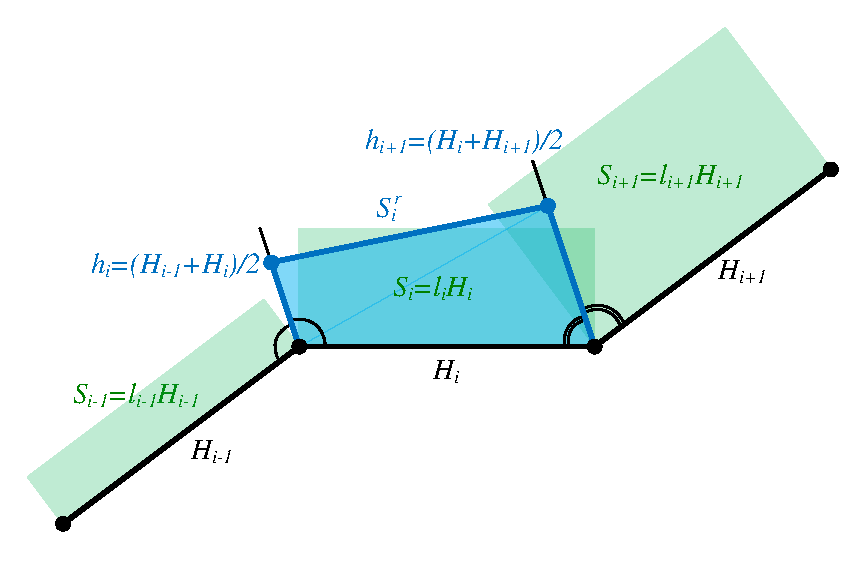
\includegraphics[width=0.45\textwidth]{pics/text_1_remesh_2d/remesh_rectangles.pdf}
&
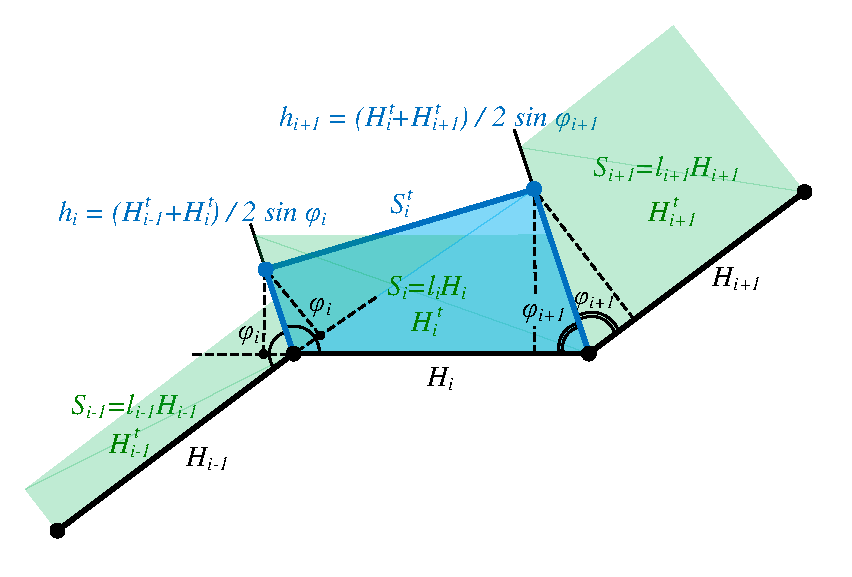
\includegraphics[width=0.45\textwidth]{pics/text_1_remesh_2d/remesh_trapeziums.pdf}
\end{tabular}
\singlespacing
\captionstyle{center}\caption{Перестроение поверхности методом прямоугольников (слева) и трапеций (справа).}
\label{fig:text_1_remesh_2d_rectangles_and_trapeziums}
\end{figure}

В качестве первого метода перестроения поверхности рассматривается приближение, при котором целевая площадь для $i$-ой ячейки представлена прямоугольником со сторонами $l_i$ и $H_i$.
В качестве величины смещения узла берется среднее арифметичское двух высот инцидентных ячеек $h_i = \frac{H_{i - 1} + H_i}{2}$ (рис.~\ref{fig:text_1_remesh_2d_rectangles_and_trapeziums} слева).
Этот метод перестроения поверхности будем называть \textit{методом прямогольников}.
Заметаемая $i$-ой ячейкой площадь при использовании метода прямоугольников обозначается $S_i^r$, также используются обозначения $\Delta_i^r = S_i^r - T_i$, $\delta_i^r = \frac{\Delta_i^r}{T_i}$.

В качестве второго метода перестроения поверхности рассматривается \textit{метод трапеций}.
В методе трапеций целевая площадь $i$-ой ячейки представляется трапецией с площадью $T_i = l_i H_i$.
Боковые стороны этой трапеции лежат на направлениях движения двух узлов, инцидентных рассматриваемой ячейке.
Высота трапеции $H_i^t$ находится с помощью решения квадратного уравнения.
После построения трапеций для всех ячеек сетки у каждого узла появляются две новые потенциальные позиции для сдвига (образованные ячейкой слева и ячейкой справа).
В качестве финальной новой позиции выбирается их среднее значение (рис.~\ref{fig:text_1_remesh_2d_rectangles_and_trapeziums} справа).
Величина смещения узла определяется как $h_i = \frac{H_{i - 1}^t + H_i^t}{2 \sin \phi_i}$.
Заметаемая $i$-ой ячейкой площадь при использовании метода трапеций обозначается $S_i^t$, также используются обозначения $\Delta_i^t = S_i^t - T_i$, $\delta_i^t = \frac{\Delta_i^t}{T_i}$.

\begin{figure}[ht]
\centering
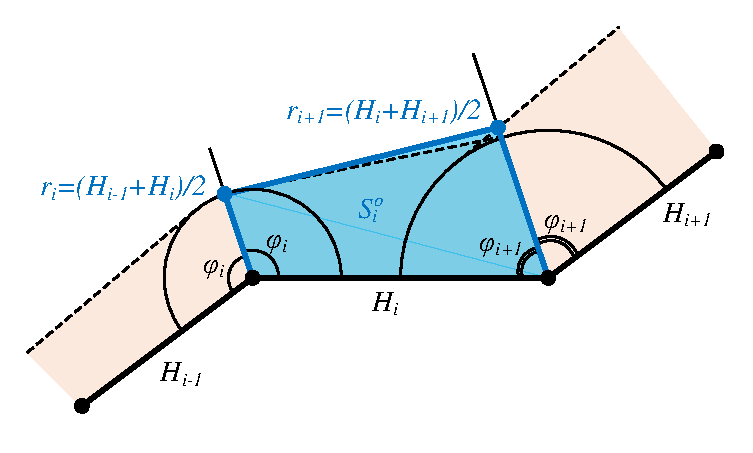
\includegraphics[width=0.5\textwidth]{pics/text_1_remesh_2d/remesh_okrestnost.pdf}
\singlespacing
\captionstyle{center}\caption{Перестроение поверхности методом окрестностей.}
\label{fig:text_1_remesh_2d_okrestnost}
\end{figure}

Предлагается новый метод перестроения поверхностной сетки, называемый \textit{методом окрестностей}.
В этом методе рассматривается \textit{фронт движения сетки} (рис.~\ref{fig:text_1_remesh_2d_okrestnost}).

При этом фронтом движения узла с номером $i$ считается сфера с центром в этом узле и радиусом $r_i = \frac{H_{i - 1} + H_i}{2}$.
Под фронтом движения ячейки сетки понимается выпуклая оболочка фронтов движения инцидентных ей узлов.
Тогда фронтом движения сетки является объединение фронтов движения всех ее ячеек.
В качестве нового положения узла берется пересечение направления смещения узла и границы фронта движения сетки.
Заметаемая $i$-ой ячейкой площадь при использовании метода окрестностей обозначается $S_i^o$, также используются обозначения $\Delta_i^o = S_i^o - T_i$, $\delta_i^o = \frac{\Delta_i^o}{T_i}$.

Приводится теоретическая оценка точности приближенных методов перестроения поверхности.
Оценка проводится для модельной расчетной сетки, которая удовлетворяет следующим требованиям.
Все ячейки сетки одинаковые и имеют длину $l$.
Для любой ячейки $AB$ и ее соседей $A_2A$ и $BB_2$ углы $\angle (\overline{BA}, \overline{AA_2})$ и $\angle (\overline{AB}, \overline{BB_2})$ являются постоянной величиной и равны $\alpha$ (для выпуклой сетки $\alpha > 0$, для вогнутой $\alpha < 0$).
Величины смещений ячеек $A_2A$, $AB$ и $BB_2$ равны $H_{i - 1}$, $H_i$ и $H_{i + 1}$ соответственно.
Оценка проводится для постоянного изменения смещения ячейки $\Delta H = H_i - H_{i - 1} = H_{i + 1} - H_i$.

\begin{figure}[ht]
\centering
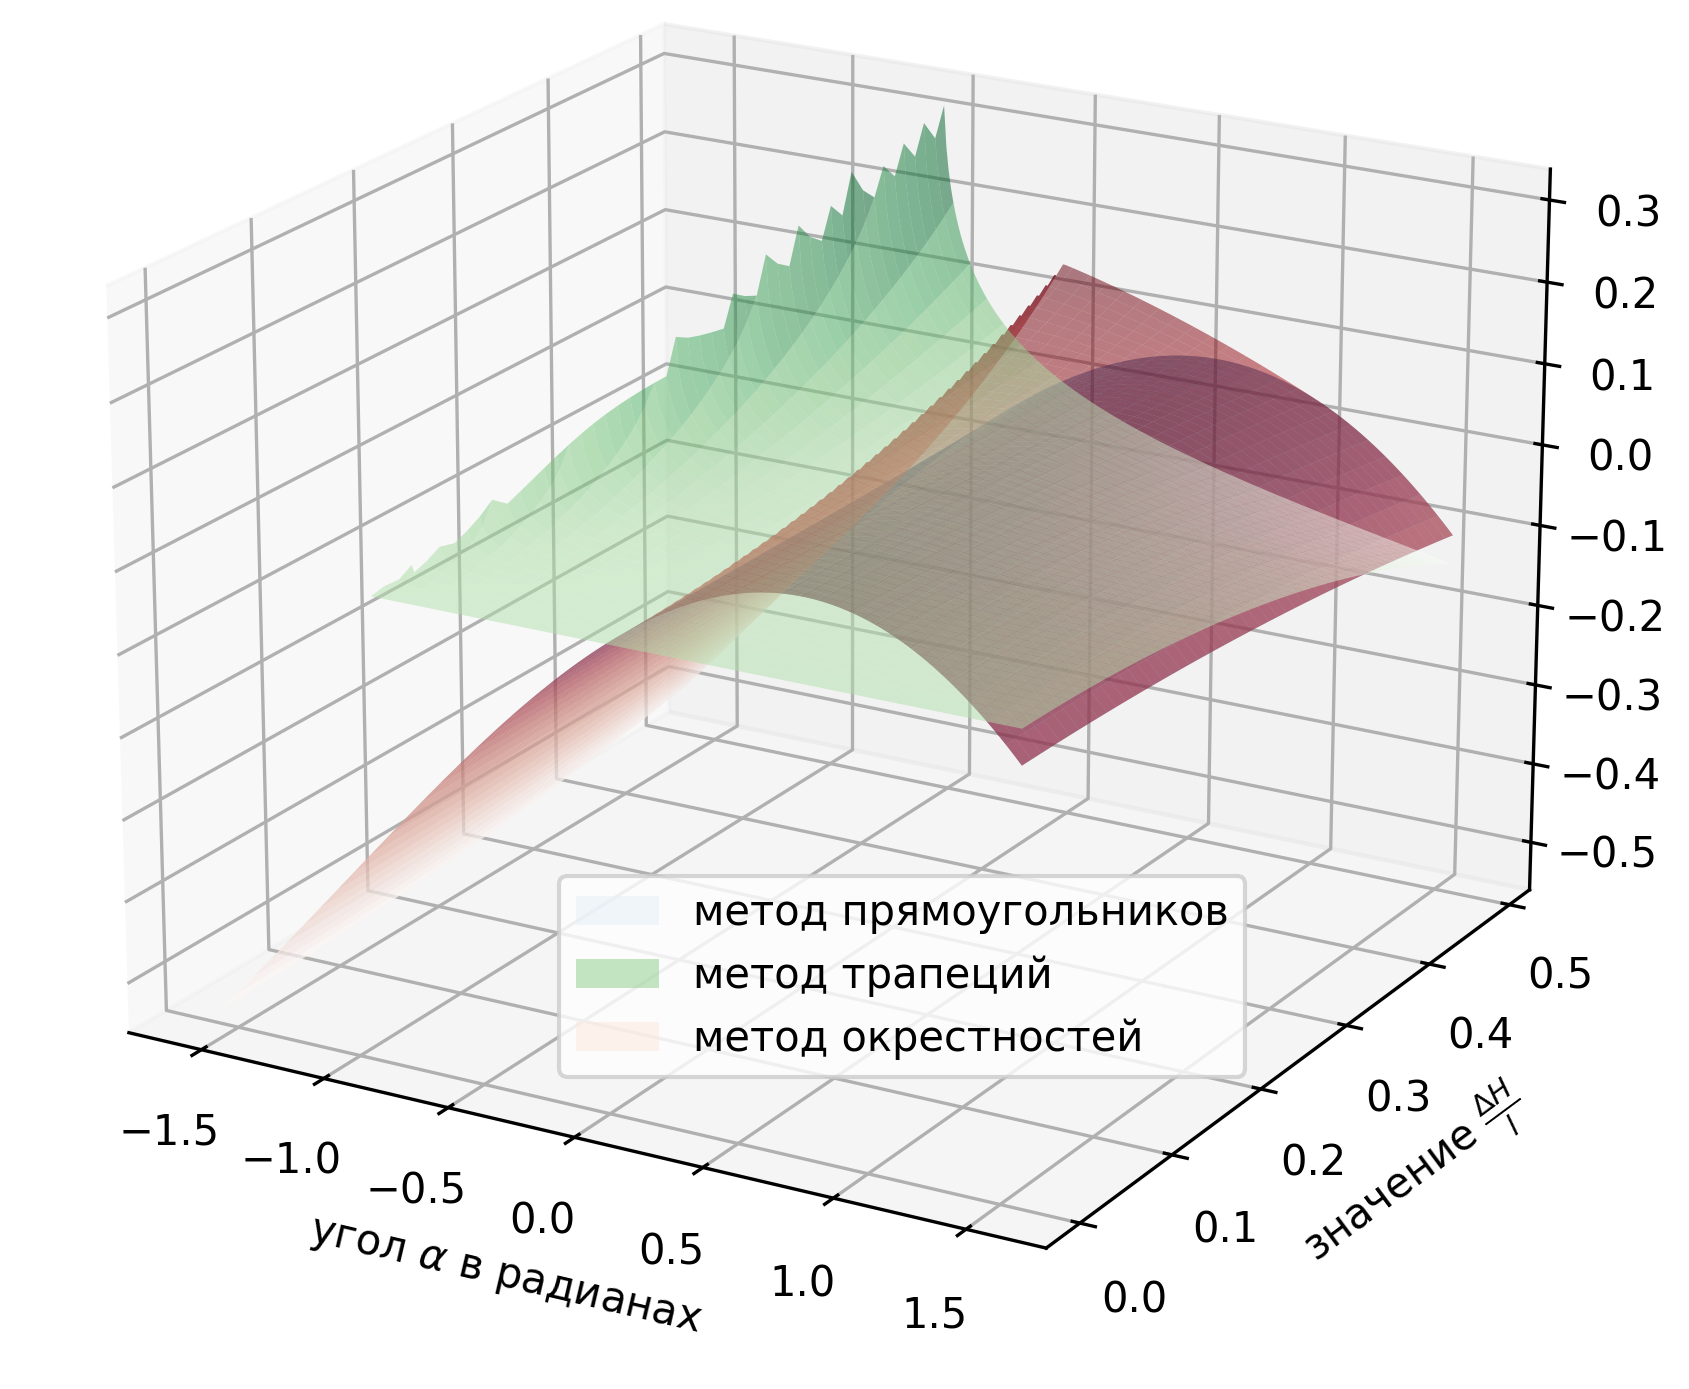
\includegraphics[width=0.6\textwidth]{pics/text_1_remesh_2d/remesh_3d_chart.png}
\singlespacing
\captionstyle{center}\caption{Графики поверхностнй $\delta_i^r(\alpha, \frac{\Delta H}{l})$, $\delta_i^t(\alpha, \frac{\Delta H}{l})$, $\delta_i^o(\alpha, \frac{\Delta H}{l})$ при фиксированном значении $H = \frac{l}{2}$.}
\label{fig:text_1_remesh_3d_main_chart}
\end{figure}

Для методов прямоугольников и трапеций, а также для предложенного метода окрестностей перестроения сетки получены зависимости $\delta_i^r(\alpha, \frac{\Delta H}{l})$, $\delta_i^t(\alpha, \frac{\Delta H}{l})$, $\delta_i^o(\alpha, \frac{\Delta H}{l})$ и проведен их анализ, представленный на рис.~\ref{fig:text_1_remesh_3d_main_chart} и рис.~\ref{fig:text_1_remesh_fix_alfa_chart}.

Из рис.~\ref{fig:text_1_remesh_3d_main_chart} можно отметить, что при $\Delta H = 0$ метод трапеций по определению абсолютно точен.
Также отметим, что при $\Delta H = 0$ отклонения $\delta_i^r$ и $\delta_i^o$ практически совпадают.

\begin{figure}[ht]
\centering
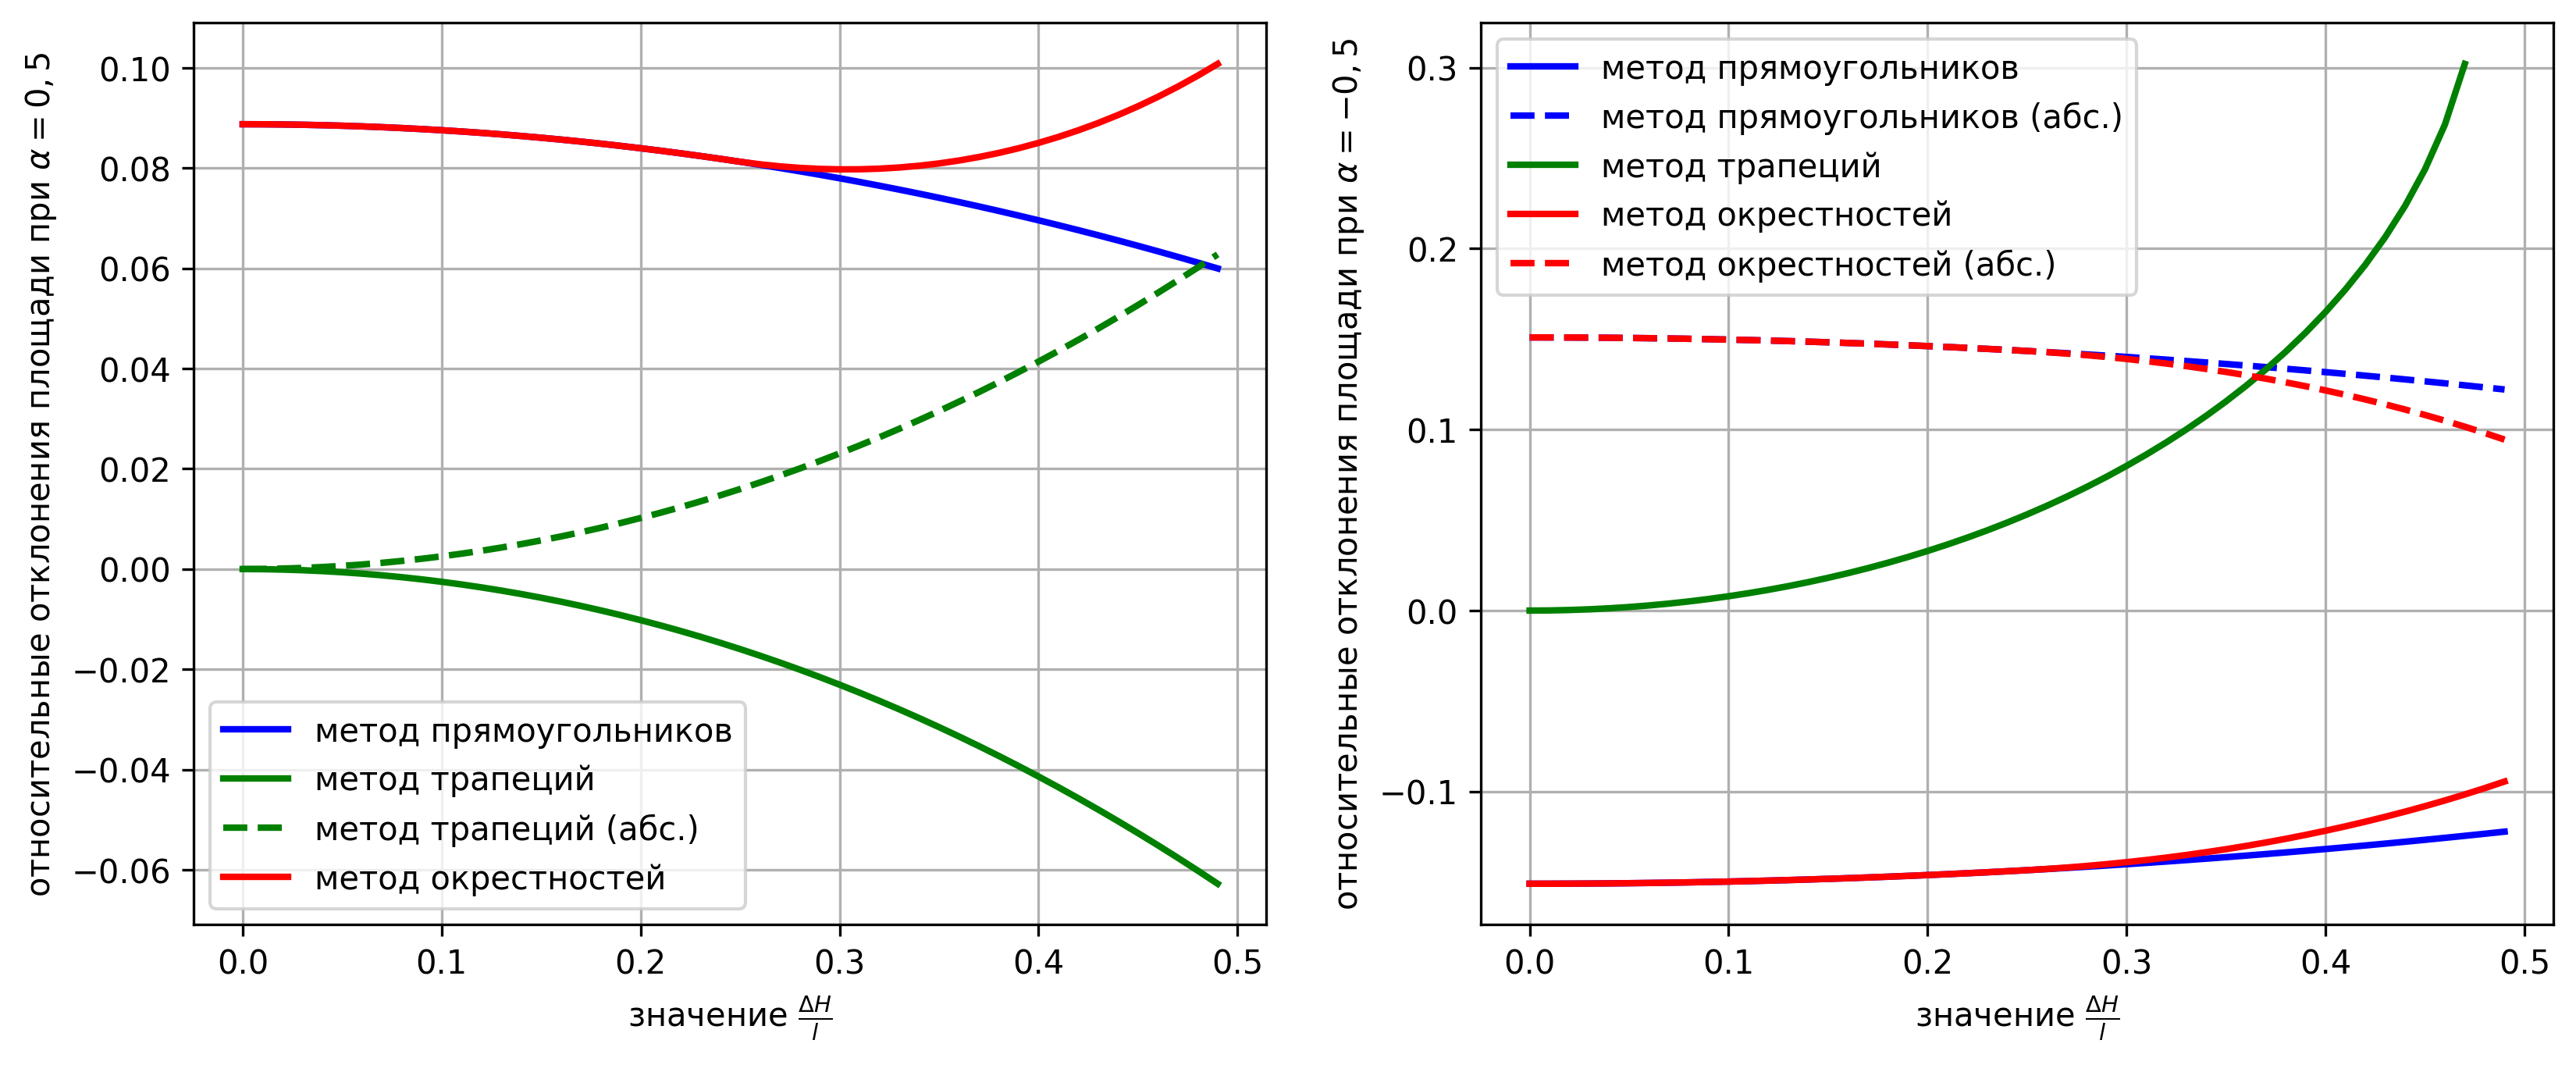
\includegraphics[width=1.0\textwidth]{pics/text_1_remesh_2d/remesh_fix_alfa_chart.png}
\singlespacing
\captionstyle{center}\caption{Графики поверхностнй $\delta_i^r(\frac{\Delta H}{l})$, $\delta_i^t(\frac{\Delta H}{l})$, $\delta_i^o(\frac{\Delta H}{l})$ при фиксированных значениях $\alpha = 0,5$ (слева) и $\alpha = -0,5$ (справа).}
\label{fig:text_1_remesh_fix_alfa_chart}
\end{figure}

Дополнительно приводятся зависимости $\delta_i^r$, $\delta_i^t$, $\delta_i^o$ от $\frac{\Delta H}{l}$ при фиксированных значениях $\alpha = 0,5$ (для выпуклой сетки) и $\alpha = -0,5$ (для вогнутой сетки) (рис.~\ref{fig:text_1_remesh_fix_alfa_chart}).
Из рисунка видно, что метод трапеций перестроения поверхности при небольших значениях $\frac{\Delta H}{l}$ наиболее точен, а точность методов прямоугольников и окрестностей достаточно близки.

Приведены оценки сглаживания острых пиков и впадин для рассмотренных методов перестроения сетки (методы прямоугольников, трапеций и окрестностей).
Для этого рассматривается расчетная сетка с одинаковыми ячейками-отрезками длины $l$.

Для оценки сглаживания острых пиков считается, что сетка является абсолютно плоской за исключением двух соседних ячеек, которые образуют острый пик с углом $2 \alpha$ (рис.~\ref{fig:text_1_remesh_2d_peak_cavern_general} слева).
Аналогично для оценки сглаживания впадин считается, что сетка является абсолютно плоской за исключением двух соседних ячеек, которые образуют впадину с углом $2 \alpha$ (рис.~\ref{fig:text_1_remesh_2d_peak_cavern_general} справа)

\begin{figure}[ht]
\centering
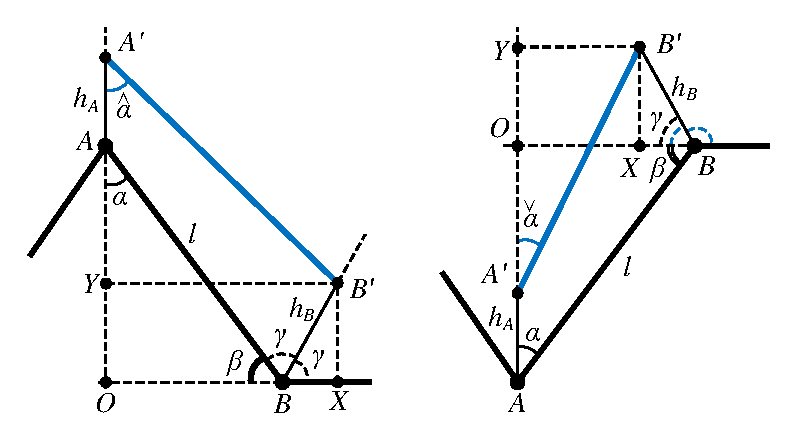
\includegraphics[width=0.6\textwidth]{./pics/text_1_remesh_2d/peak-cavern-general.pdf}
\singlespacing
\captionstyle{center}\caption{Оценка сглаживания угла при остром пике (слева) \\ и при впадине (справа).}
\label{fig:text_1_remesh_2d_peak_cavern_general}
\end{figure}

В этих условиях получены зависимости сглаженного угла при остром пике
\begin{equation}
\hat{\alpha}_1(h_A, h_B) = \arctg \frac{l \sin \alpha + h_B \cos \gamma}{l \cos \alpha + h_A - h_B \sin \gamma}
\end{equation}
а также при впадине 
\begin{equation}
	\begin{aligned}
		& \check{\alpha}_1(h_A, h_B) = \arctg \frac{l \sin \alpha - h_B \cos \gamma}{l \cos \alpha - h_A + h_B \sin \gamma} \\
		& \arcsin \frac{h_B \left( \sqrt{8 l^2 + h_B^2} - h_B \right)}{4 l^2} \le \alpha \le \arccos \frac{h_A}{l}
	\end{aligned}
\end{equation}

\begin{figure}[ht]
\centering
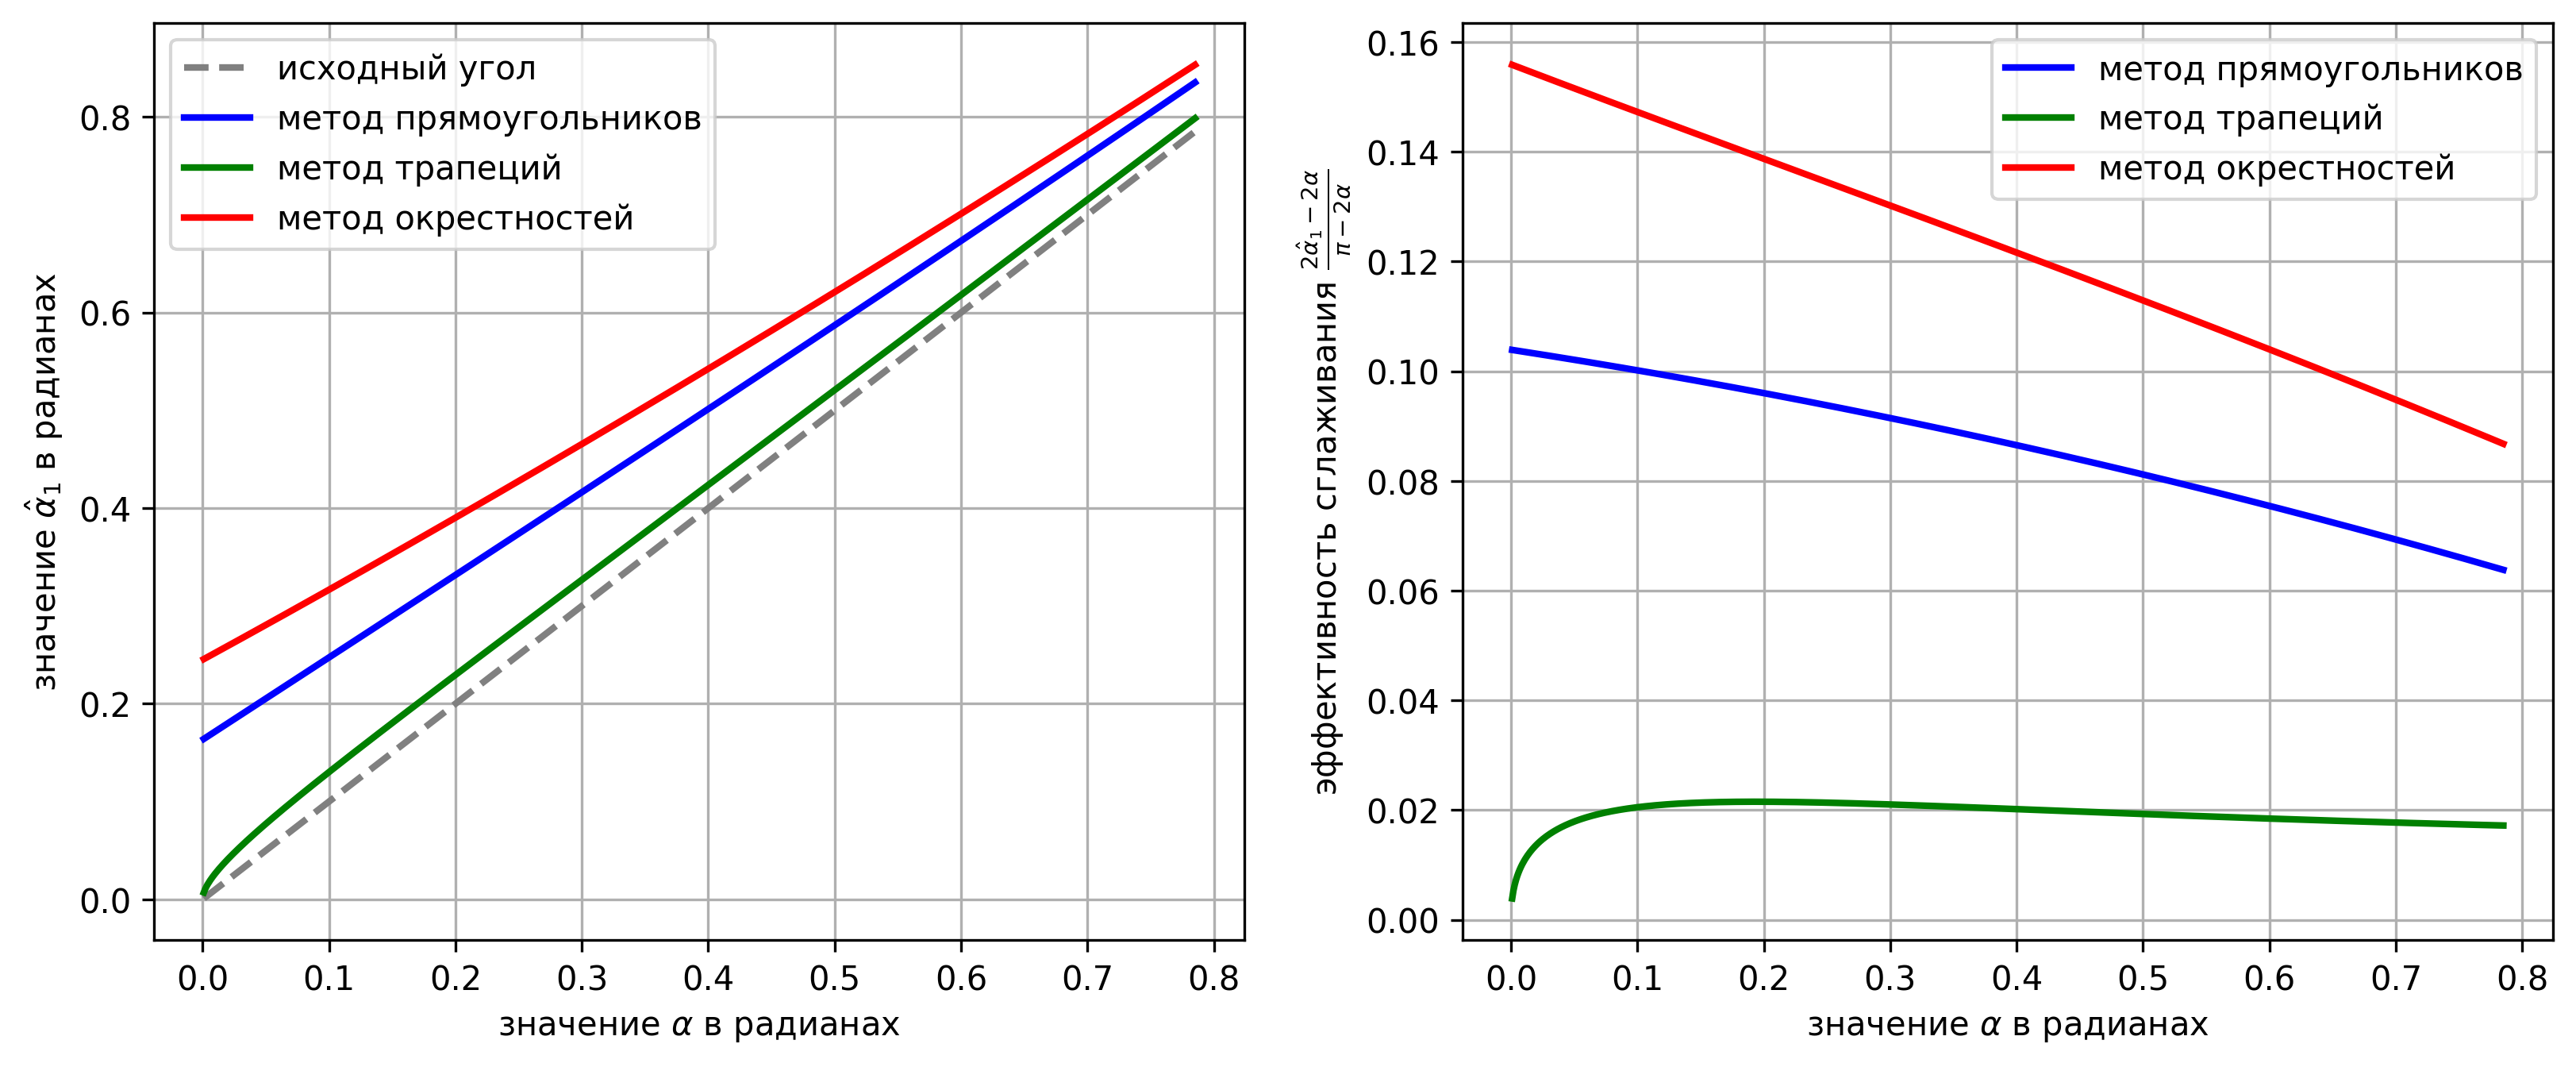
\includegraphics[width=1.0\textwidth]{./pics/text_1_remesh_2d/peak-methods-chart.png}
\singlespacing
\captionstyle{center}\caption{Сравнение сглаживания острого пика для методов прямоугольников, трапеций и окрестностей.}
\label{fig:text_1_remesh_2d_peak_methods_chart}
\end{figure}

\begin{figure}[!ht]
\centering
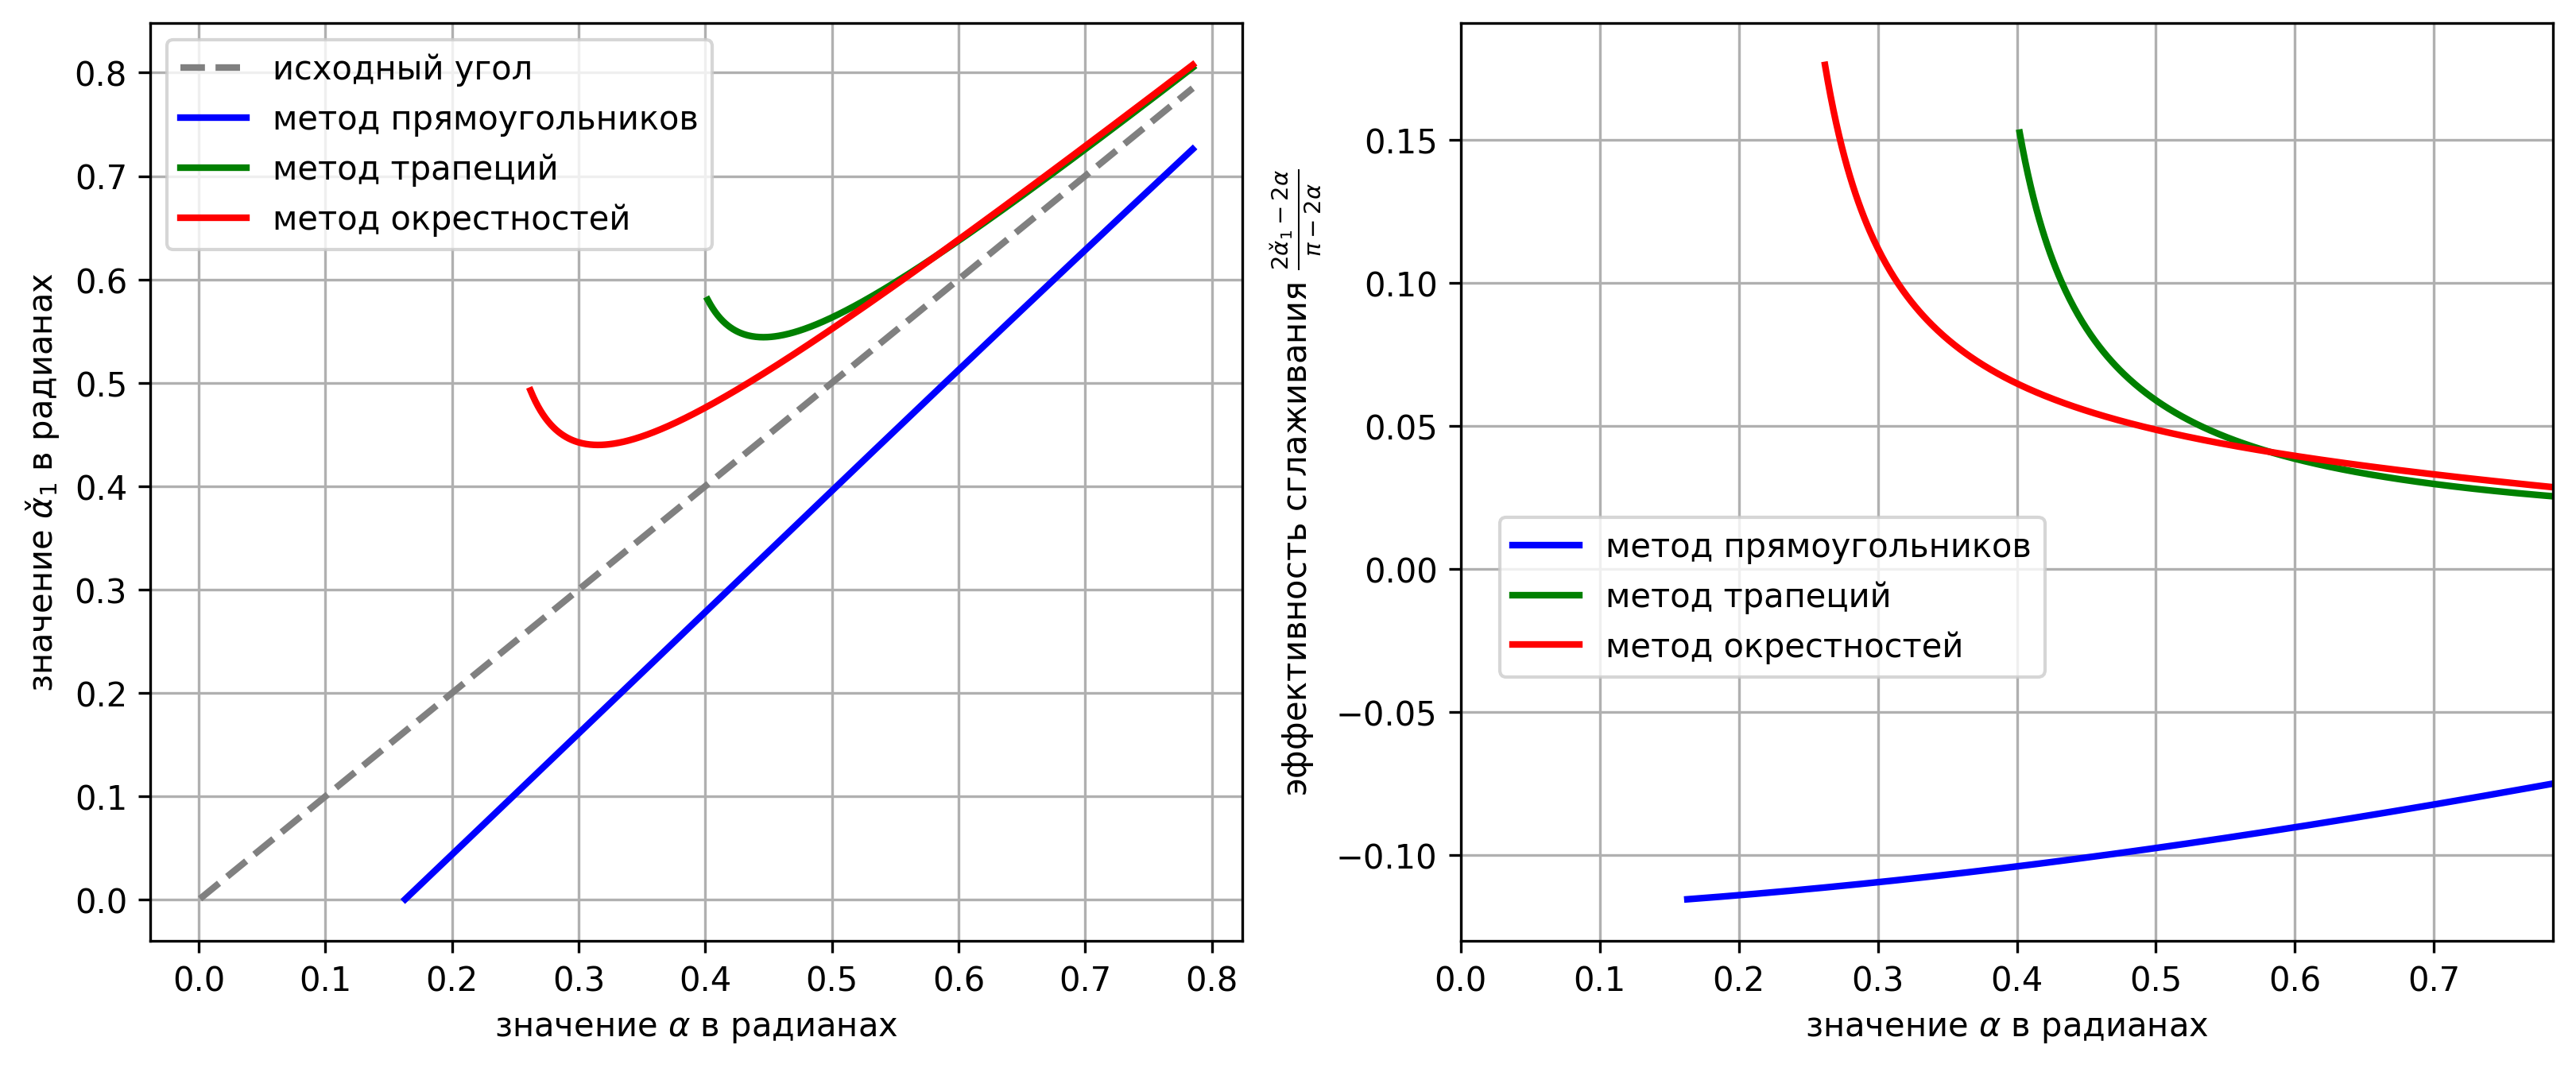
\includegraphics[width=1.0\textwidth]{./pics/text_1_remesh_2d/cavern-methods-chart.png}
\singlespacing
\captionstyle{center}\caption{Сравнение сглаживания впадины для методов прямоугольников, трапеций и окрестностей.}
\label{fig:text_1_remesh_2d_cavern_methods_chart}
\end{figure}

На рис.~\ref{fig:text_1_remesh_2d_peak_methods_chart} приведены графики сравнения методов прямоугольников, трапеций и окрестностей в применении к сглаживанию острых пиков.
При этом используется фиксированная величина смещения ячейки $H = \frac{l}{4}$.
На графике слева показана зависимость изменения сглаженного угла $\hat{\alpha}_1$ от $\alpha$.
На графике справа показана эффективность сглаживания, выраженная формулой $\frac{2 \hat{\alpha}_1 - 2 \alpha}{\pi - 2 \alpha}$ (значение 1 означает полное сглаживание пика до угла $\hat{\alpha}_1 = \frac{\pi}{2}$).
Можно отметить, что наиболее эффективное сглаживание угла $\alpha$ обеспечивает метод окрестностей.
Дополнительно заметим, что использование метода трапеций для малых углов $\alpha$ приводит к неконтролируемому росту $h_A$, что делает применение этого метода неприемлемым.

На рис.~\ref{fig:text_1_remesh_2d_cavern_methods_chart} приведены графики сравнения методов прямоугольников, трапеций и окрестностей в применении к сглаживанию впадин.
При этом используется фиксированная величина смещения ячейки $H = \frac{l}{4}$.
На графике слева показана зависимость изменения сглаженного угла $\check{\alpha}_1$ от $\alpha$.
На графике справа показана эффективность сглаживания, выраженная формулой $\frac{2 \check{\alpha}_1 - 2 \alpha}{\pi - 2 \alpha}$ (значение 1 означает полное сглаживание пика до угла $\hat{\alpha}_1 = \frac{\pi}{2}$).
Можно отметить, что метод прямоугольников не сглаживает угол, а наоборот, делает его еще более острым (значение эффективности сглаживания меньше нуля).
Метод трапеций показывает лучшую эффективность сглаживания, но с меньшей областью применимости.

Из приведенных оценок на рис.~\ref{fig:text_1_remesh_2d_peak_methods_chart} и рис.~\ref{fig:text_1_remesh_2d_cavern_methods_chart} можно сделать вывод, что метод окрестностей перестроения является оптимальным с точки зрения точноси перестроения и способности сглаживания дефектов сетки.

%----------------------------------

В п.~1.3 рассматривается постановка задачи перестроения поверхностной неструктурированной расчетной сетки в трехмерном случае при фиксированных направлениях смещения узлов.
Задача рассматривается в постановка, когда в каждой ячейке сетки известен объем накопленного льда ($V$).
Для каждого узла сетки $N$ требуется найти его новое положение в пространстве $N'$, чтобы для каждой ячейки с узлами $ABC$ объем пространства, ограниченный фигурой $ABCA'B'C'$ соответствовал объему льда, накопленному в этой ячейке.
Таким образом, поставновка задачи в трехмерном случае аналогично двумерной постановке.

Для трехмерной постановки рассматриваются классические приближенные методы перестроения, аналогичные двумерному случаю.
В \textit{методе призм} перестроения поверхности (аналог метода прямоугольников в двумерной постановке) в качестве приближения заметаемого объема рассматривается призма, одним из оснований которой является ячейка (рис.~\ref{fig:text_1_remesh3_rect} слева).
В \textit{методе пирамид} перестроения поверхности (аналог метода трапеций в двумерной постановке) в качестве приближения заметаемого объема рассматривается призматоид, одним из оснований которого является ячейка, в боковые стороны направлены вдоль направлений смещения узлов (рис.~\ref{fig:text_1_remesh3_rect} справа).

\begin{figure}[h]
\centering
\begin{tabular}{ll}
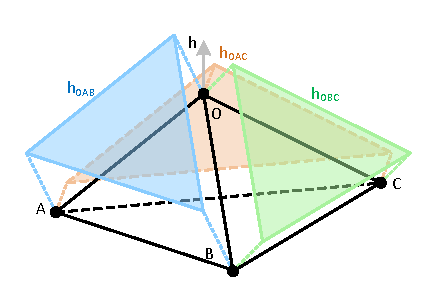
\includegraphics[width=0.43\textwidth]{pics/text_1_remesh_3d/pic_classical_methods_prisms.pdf}
&
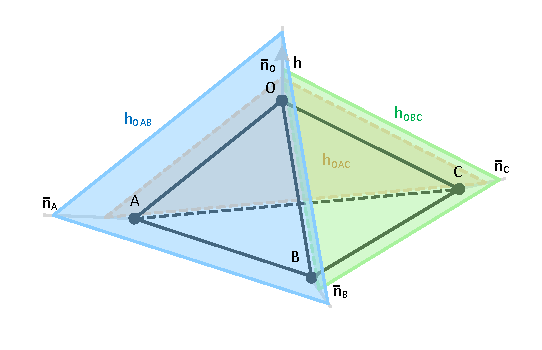
\includegraphics[width=0.52\textwidth]{pics/text_1_remesh_3d/pic_classical_methods_pyramids.pdf}
\end{tabular}
\singlespacing
\captionstyle{center}\caption{Перестроение поверхности с помощью метода призм (слева) и пирамид (справа).}
\label{fig:text_1_remesh3_rect}
\end{figure}

Также рассматриваются дополнительные вопросы перестроения поверхностной сетки.
В частности многослойный метод перестроения, в котором выполнятеся $k$ последовательных шагов перестроения сетки для величин смещения ячеек $\frac{H_i}{k}$.
Рассматриваются метод сглаживания поля нормалей для предотвращения раннего самопересечения сетки, метод сглаживания высот для устранения поверхностного шума, а также метод сглаживания сетки, позволяющий перераспределить узлы по поверхности для балансировки размера ячеек. 

%----------------------------------

В п.~1.4 предлагается метод окрестностей перестроения поверхностной неструктурированной расчетной сетки в трехмерной постановке.
Рассмотривается геометрическая задача определения новых положений узлов расчетной сетки, если для каждого узла $N$ известна скорость образования ледяного покрова $v(N)$.
Будем считать, что нарастание льда в любой точке роста льда выполняется одновременно во всех направлениях аналогично принципу Гюйгенса-Френеля распространения волн.
Таким образом, фронт распространения льда от произвольной точки $P$ через промежуток времени $\Delta t$ будет иметь форму сферы $Sphere(P, v(P)\Delta t)$.
Далее будем считать, что мы выполняем расчет новых положений узлов через некоторый фиксированный момент времени $\Delta t$, то есть для каждого узла $N$ известен радиус продвижения фронта сетки $R(N) = v(N) \Delta t$.
Радиус продвижения фронта в точке ячейки сетки будем определять как $R(P(\beta,\gamma)) = R(\beta,\gamma) = R(A) + \beta(R(B) - R(A)) + \gamma(R(C) - R(A))$.
Тогда фронтом продвижения ячейки является выпуклая оболочка сфер $Sphere(P(\beta, \gamma), R(\beta, \gamma))$ для $\beta \ge 0$, $\gamma \ge 0$, $\beta + \gamma \le 1$.

\begin{figure}[!ht]
\centering
\begin{tabular}{ll}
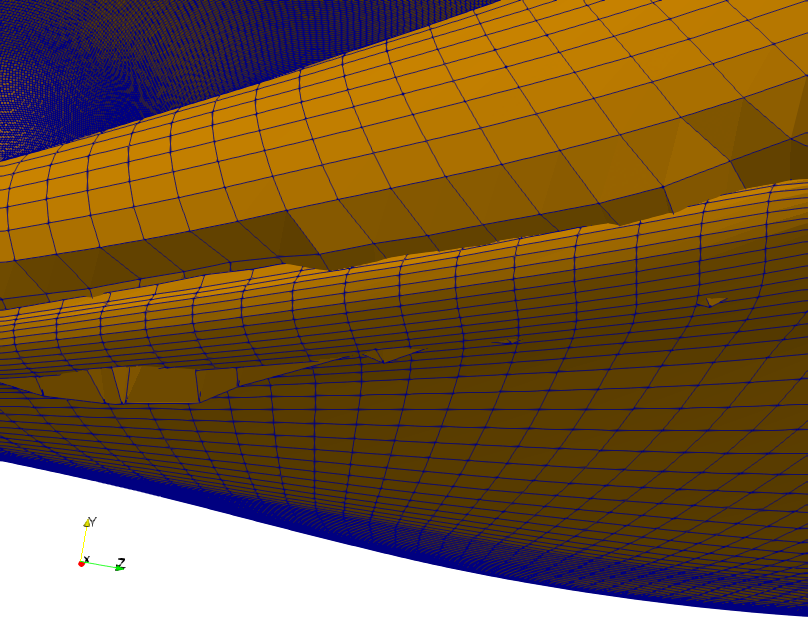
\includegraphics[width=0.45\textwidth]{pics/text_1_remesh_3d/fens1.png}
&
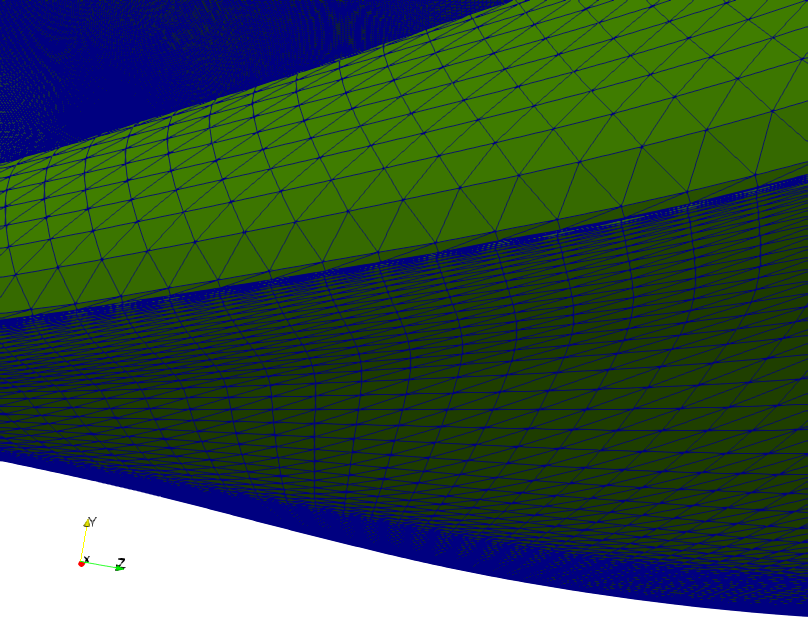
\includegraphics[width=0.45\textwidth]{pics/text_1_remesh_3d/crys1.png} \\
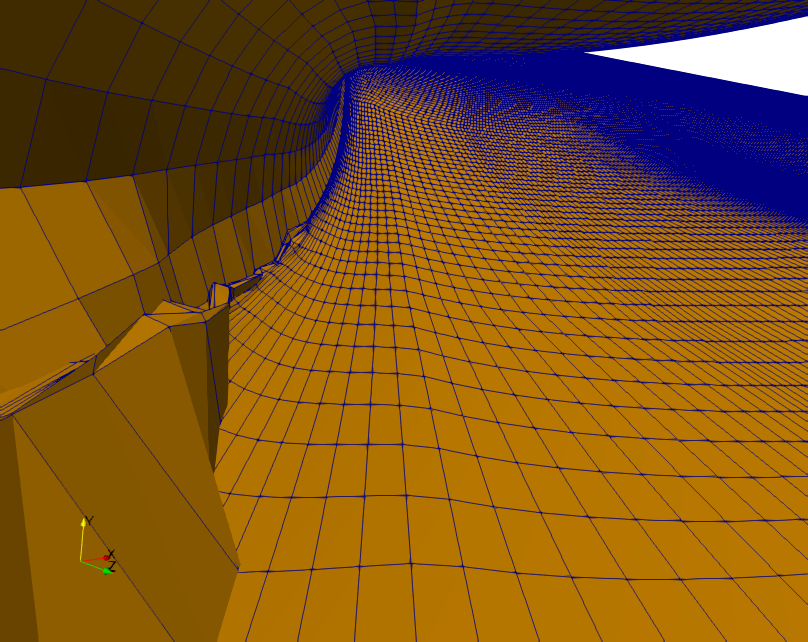
\includegraphics[width=0.45\textwidth]{pics/text_1_remesh_3d/fens2.png}
&
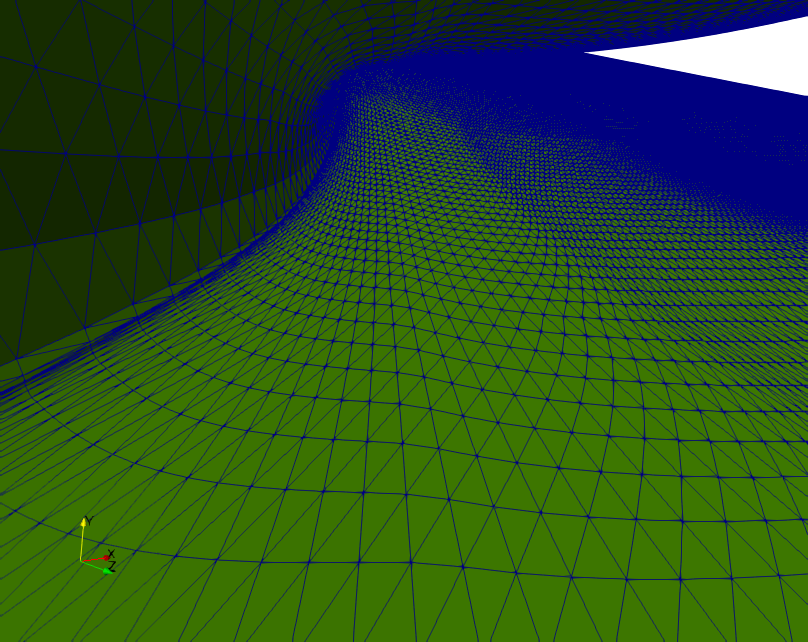
\includegraphics[width=0.45\textwidth]{pics/text_1_remesh_3d/crys2.png}
\end{tabular}
\singlespacing
\captionstyle{center}\caption{Эффект сглаживания дефектов при перестроении методом окрестностей (справа) в сравнении с программным комплексом FENSAP.}
\label{fig:text_1_remesh3_with_fensap}
\end{figure}

Рассматривается задача нахождения точек пересечения траектории движения узла ячейки $A$ ($\overline{P}(\alpha) = \overline{A} + \alpha \overline{D}$ при $\alpha \ge 0$) с фронтом продвижения ячейки.
Эти точки находятся из решения уравния $|(\overline{A} + \alpha \overline{D}) - \overline{C}(\beta, \gamma)| = R(\beta, \gamma)$ относительно $\alpha$.
Наибольший корень этого уравнения может быть выражен явно (с учетом условия $|\overline{D}| = 1$)
\begin{equation}
	\begin{aligned}
		& \alpha(\beta, \gamma) = k_{\beta} \beta + k_{\gamma} \gamma + \sqrt{T} \\
		& T = q_{\beta^2} \beta^2 + q_{\gamma^2} \gamma^2 + q_{\beta \gamma} \beta \gamma + q_{\beta} \beta + q_{\gamma} \gamma + q \\
		& k_{\beta} = (\overline{D}, \overline{AB}), \ k_{\gamma} = (\overline{D}, \overline{AC}) \\
		& q_{\beta^2} = (\overline{D}, \overline{AB})^2 - |\overline{AB}|^2 + R_{AB}^2, \ q_{\gamma^2} = (\overline{D}, \overline{AC})^2 - |\overline{AC}|^2 + R_{AC}^2 \\
		& q_{\beta \gamma} = 2 \left( (\overline{D}, \overline{AB}) (\overline{D}, \overline{AC}) - (\overline{AB}, \overline{AC}) + R_{AB}R_{AC} \right) \\
		& q_{\beta} = 2 R_A R_{AB}, \ q_{\gamma} = 2 R_A R_{AC}, \ q = R_A^2
	\end{aligned}
\end{equation}

Требуемая точка пересечения соответствует максимальному значению $\alpha(\beta, \gamma)$ при ограничениях $\beta \ge 0$, $\gamma \ge 0$, $\beta + \gamma \le 1$.
Изложенная последовательность действий касается определения смещения узла с учетом только одной инцидентной ячейки.
При рассмотрении отдельного узла расчетной сетки требуется вычислить смещение этого узла относительно каждой инцидентной ячейки и выбрать среди этих смещений максимальное.

Предложенный метод окрестностей перестроения поверхностной неструктурированной расчетной сетки в трехмерном случае, также как и его двумерный аналог, обладает способностью сглаживания дефектов расчетной сетки при приемлемой точности перестроения (рис.~\ref{fig:text_1_remesh3_with_fensap}).

%----------------------------------

В п.~1.5 рассматривается проблема устранения самопересечений поверхностной неструктурированной расчетной сетки.
Самопересечение является критическим дефектом сетки, при котором невозможно производить дальнейшие вычисления по моделированию ледообразования, поэтому самопересечения необходимо удалять.
В общем случае предотвратить самопересечение невозможно, так как в процессе ледообразования при активном нарастании льда возможно переречение одних ледяных наростов с другими ледяными наростами.
Таким образом, для адекватного моделирования процесса ледообразования необходимо уметь корректно обрабатывать самопересечения расчетной сетки, чтобы после возникновения самопересечения можно быть продолжать выполнение расчетов.

\begin{figure}[!ht]
\centering
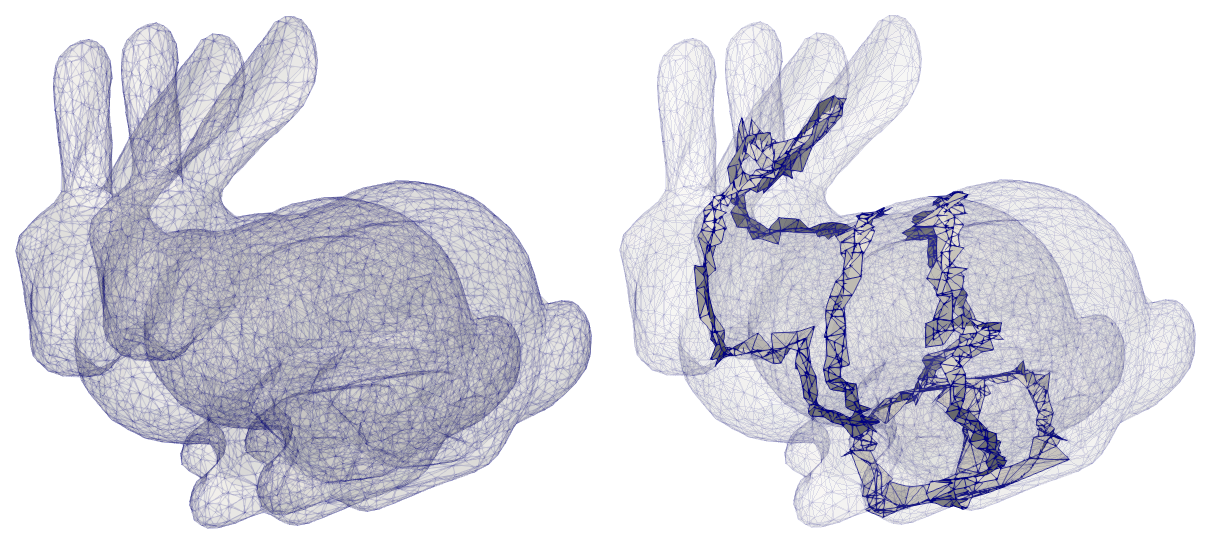
\includegraphics[width=1.0\textwidth]{./pics/text_1_int/bunnies_dbl.png}
\singlespacing
\captionstyle{center}\caption{Устранение самопересечений в случае достаточной точности определения пересечения пар треугольников.}
\label{fig:text_1_int_1}
\end{figure}

Предлагаются два подхода к устранению самопересечений.
Сначала требуется найти всех пары пересекающихся ячеек сетки.
Для этого используется иерархическая структура дерева треугольников, позволяющая избежать проверки на пересечение каждой пары ячеек.
Основной проблемой при поиске пересечений двух треугольников являются ошибки точности, из-за которых может быть принято ошибочное решение о пересечении: попадание узла сетки на ребро или на ячейку, пересечение двух ребер сетки, пересечение ячеек под острым углом.
В некоторых случаях такие конфликты можно разрешить локальной коррекцией положения узлов.
Если конфликты удается разрешить, и все пары пересекающися ячеек определены корректно, то все пересекающиеся ячейки сетки разбиваются на более мелкие ячейки по всем точкам пересечения, после чего внешняя часть сетки определяется путем обхода ячеек (рис.~\ref{fig:text_1_int_1}).

\begin{figure}[!ht]
\centering
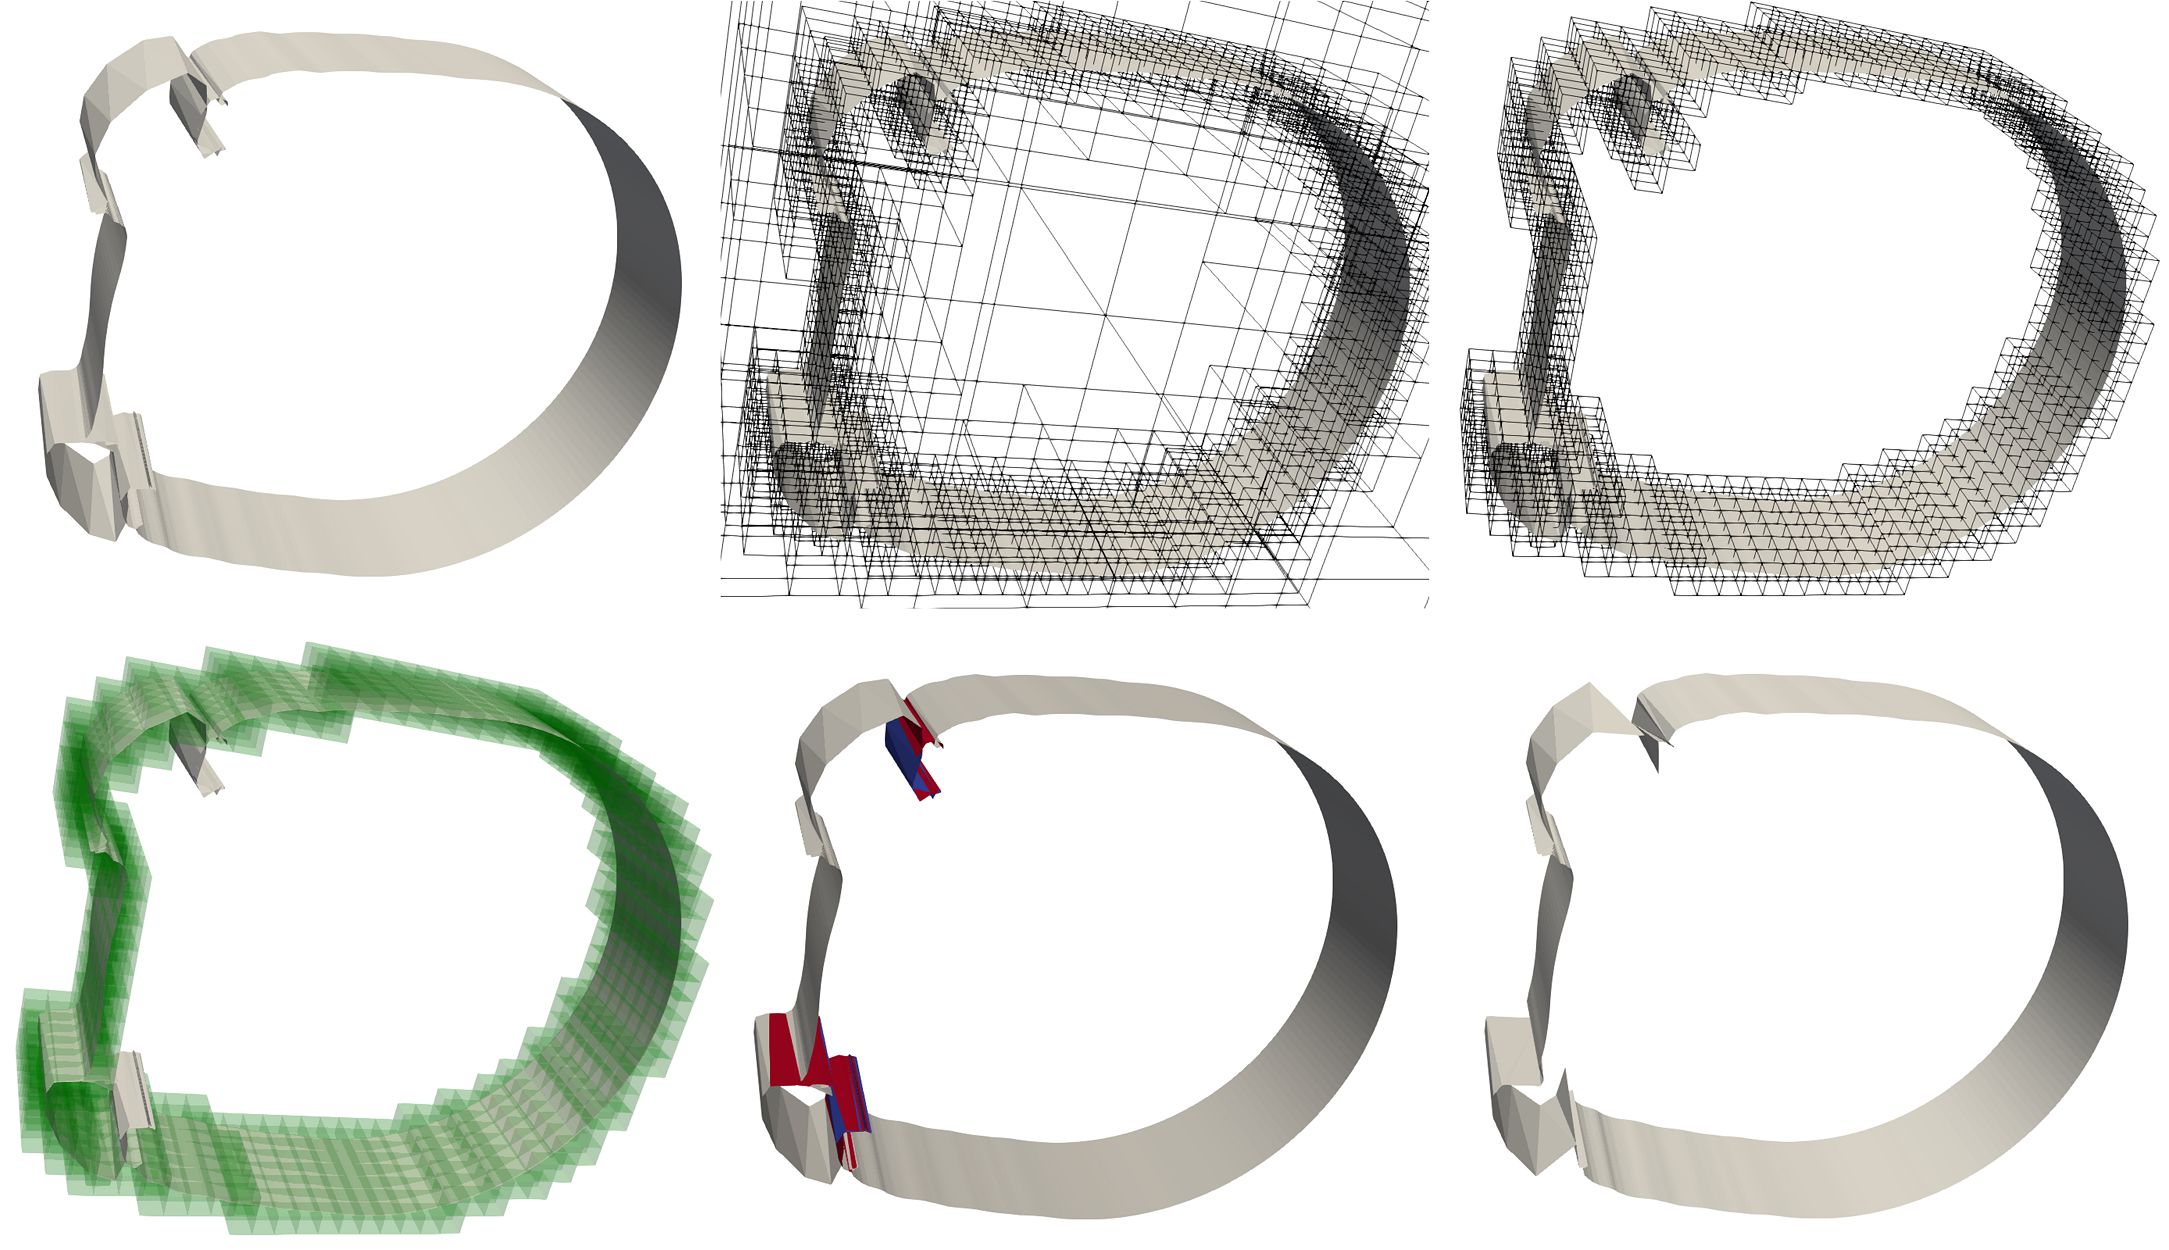
\includegraphics[width=1.0\textwidth]{./pics/text_1_int/wing_all.png}
\singlespacing
\captionstyle{center}\caption{Устранение самопересечения с использованием подложки поверхностной сетки.}
\label{fig:text_1_int_2}
\end{figure}

При перестроении поверхности для задачи ледообразования расчетная сетка, как правило, отличается низким качеством -- в ней могут присутствовать ячейки с углами, близкими к $0$ или $\pi$, что препятствует корректному определению точек пересечения.
В этом случае используется второй подход к устранению самопересечений.
В пространстве строится восьмеричное дерево вложенных кубов, называемое \textit{подложкой}, где корень охватывает всю поверхность, а дочерние кубы строятся только в случае пересечения с сеткой.
Минимальный размер ячейки подложки выбирается меньше минимального ребра поверхностной сетки.
Далее определяется внешний слой кроны подложки и все ячейки, не пересекающие этот слой, помечаются как кандидаты на удаление из сетки.
Также помечаются все ячейки, пересекающие другие ячейки в сетке.
После чего выполняется шаг стягивания сетки по ребрам, входящим в помеченную область.
После этого процесс повторяется итерационно, пока расчетная сетка не будет избавлена от самопересечений.
Такой подход не гарантирует устранение самопересечений, однако в отдельных случаях он оказывается применимым (например для расчетов на псевдотрехмерных профилях, рис.~\ref{fig:text_1_int_2}).

%----------------------------------

В п.~1.6 рассматривается проблема сопряжения поверхностной сетки с объемной сеткой для определения поля скоростей вокруг обтекаемого тела.
При расчете обледенения крайне важным элементом данных является поле скоростей в области, окружающей рассматриваемую поверхность.
Поле скоростей вблизи поверхности влияет на движение жидкой пленки по поверхности, что существенным образом определяет картину обледенения.
Также при использовании модели вторичного увлажнения отскочившие от поверхности капли попадают в свободный поток, и поле скоростей необходимо для расчета траектории их движения и зоны вторичного выпадения.
Так как при перестроении поверхностной сетки построение согласованной объемной сетки является затратной процедурой, то для возможности продолжения расчетов предлагается метод погруженной границы с фиктивными ячейками.

%----------------------------------

В п.~1.7 рассматривается \textit{метод погруженной границы} с использованием \textit{фиктивных ячеек} в трехмерной постановке.
В предлагаемом методе строится подложка поверхностной сетки, в которой ячейки кроны подложки разделяются на три категории ячеек 
Внешними ячейками будем называть те ячейки, которые целиком лежат вне тела.
Внутренние ячейки лежат целиком внутри тела, все остальные ячейки пересекают границу тела и являются граничными.
В методе погруженной границы с использованием фиктивных ячеек из граничных ячеек выделяются ячейки, для которых меньшая часть объема находится вне тела, а большая -- внутри тела.
Такие ячейки называются фиктивными.
Это разделение ячеек на классы является первичным и весьма приближенным, так как после коррекции некоторые внутренние ячейки могут быть также переведены в разряд фиктивных (в процессе проведения вычислений должно выполняться следующее требование: соседями внутренних ячеек не могут являться ни граничные, ни внешние ячейки).
На каждой итерации расчетов для фиктивных ячеек требуется выполнить аппроксимацию газодинамических величин (плотность, давление, вектор скорости), чтобы эти фиктивные ячейки могли быть использованы для определения потоков между ними и соседними с ними граничными и внешними ячейками.
Аппроксимация скалярных и векторных газодинамических величин в фиктивных ячейками выполняется с помощью шаблонов, в которые входят три внешние ячейки, а также точка поверхности, в которой известно направление нормали.

%---------------------------------------------------------------------------------------------------

\textbf{Вторая глава} посвящена вопросам распараллеливания вычислений с передачей сообщений на различных расчетных сетках.

%----------------------------------

В п.~2.1 приводятся основные показатели качества декомпозиции расчетной сетки при распределении ячеек по \textit{доменам}.

В качестве первого показателя качества декомпозиции сетки (\textit{неравномерность декомпозиции}) принимается максимальное абсолютное отклонение размера домена от теоретически возможного среднего значения $D = \max_{1 \le i \le k}{ \left( n_i - \frac{n}{k} \right) }$, где $n_i$ – количество ячеек в $i$-ом домене.
В идеальном случае равномерного распределения ячеек по доменам показатель $D$ становится равным нулю.
В худшем случае все ячейки распределяются в один домен и $D = n \left( 1 - \frac{1}{k} \right)$.
Так как абсолютный показатель не слишком удобен для сравнения разных алгоритмов декомпозиции на разных сетках, то дополнительно будем использовать показатель, который характеризует долю накладных расходов неравномерного распределения ячеек по доменам по отношении к идеальному распределению, а именно $D^{*} = \frac{D}{n / k}$.
Значение $D^{*}$ изменяется в диапазоне $[0, k - 1]$, где $D^{*} = 0$ означает идеальное распределение ячеек по доменам, а $D^{*} = k - 1$ соответствует наихудшему случаю, когда все ячейки отнесены к одному домену.
Также будем использовать величину $D^{\%} = D^{*} \cdot 100\%$ для возможности указания значения показателя в процентах.

В качестве второй характеристики качества декомпозиции будем использовать величину наиболее протяженной границы между парой доменов, или $L_{ij} = \left| \{ e \in E: \{ d(e_a), d(e_b) \} = \{ i, j \} \} \right|$, $L = \max_{1 \le i < j \le k}{L_{ij}}$, где $d(v)$ -- домен, к которому относится вершина $v$.
В идеальном случае значение характеристики $L$ может быть сколь угодно малым, даже нулевым (в случае, если сетка представляет собой $k$ одинаковых по количеству ячеек несвязных областей).
В наихудшем случае случае $L = |E|$, если ячейки распределены в два домена в шахматном порядке, и каждое ребро относится к границе между этими двумя доменами.
Наряду с показателем $L$ используется нормированный показатель $L^{*}$, определяемый как $L^{*} = \frac{L}{|E|}$, который изменяется в диапазоне $[0, 1]$ и принимает значение 0 в идельном случае, а 1 -- в наихудшем.
Также будем использовать показатель длины максимальной границы между доменами в процентах от общего количества ребер $L^{\%} = L^{*} \cdot 100\%$.

В роли дополнительной характеристики качества декомпозиции можно использовать суммарную длину границ между доменами $I = \sum_{1 \le i < j \le k}{L_{ij}}$, что соответствует общему количеству пересылаемых данных в рамках межпроцессного обмена.
Так как домены граничат между собой по ребрам дуального графа, то суммарная длина всех границ между доменами представляет собой просто количество всех ребер, инцидентных двум относящимся к разным доменам ячейкам, то есть количество междоменных ребер.
Наряду с показателем $I$ будем использовать долю междоменных ребер среди общего количества ребер сетки $I^{*} = \frac{I}{|E|}$.
Показатель $I^{*}$ также является нормированным, он изменяется в диапазоне $[0, 1]$ и принимает значение 0 в идеальном случае и 1 -- в наихудшем.
Также будем использовать показатель количества междоменных ребер в процентах от общего количества ребер $I^{\%} = I^{*} \cdot 100\%$.

%----------------------------------

В п.~2.2 рассматривается архитектура блочно-структурированной расчетной сетки с поддержкой дробления блоков.
Для этой сетки приводится иерархия входящих в ее состав элементов, а также описывается механизм организации межпроцессных обменов с возможностью сокрытия издержек на обмены за полезными вычислениями.

%----------------------------------

В п.~2.3 рассматривается жадный алгоритм распределения вычислительной нагрузки при обработке блочно-структурированной расчетной сетки между узлами гетерогенного вычислительного кластера с учетом топологии вычислительного поля.

%----------------------------------

В п.~2.4 рассматриваются вопросы распределения вычислительной нагрузки при выполнении расчетов на блочно-структурированной рассчетной сетке с дроблением блоков.

Сначала рассматривается задача распределения вычислительной нагрузки без дробления с помощью жадного алгоритма.
Рассмотрим множество $X$ вещественных чисел $x_i \ge 0$ для $i \in N$, где $N = [1, n]$.
Рассмотрим также множество индексов $j \in M$, где $M = [1, m]$.
Будем говорить, что определено разбиение множества $X$ на $m$ множеств, если введена функция $\gamma(i): N \rightarrow M$.
Множество всех функций разбиения будем обозначать $\Gamma(N, M)$.
Веса результирующих множеств будем определять естественным образом для $j \in M$: $X_j = \sum_{\substack{i \in N \\ \gamma(i) = j}}{x_i}$.

Требуется найти такую функцию разбиения $\gamma \in \Gamma(N, M)$, чтобы минимизировать наиболее тяжелое из результирующих множеств $\max_{j \in M}{X_j}$.
В жадном алгоритме будем последовательно обрабатывать все веса, начиная с наибольшего.
Каждый необработанный вес будем относить к наиболее легкому на текущий момент множеству весов.
Определим остаточный член $r_i$ для $i \in N$ по следующей формуле:
\begin{equation}
	r_i = \max{\left( x_i - \frac{1}{m} \sum_{p = i}^{n}{x_p}, 0 \right)}
\end{equation}

Тогда верно следующее утверждение.
При использовании жадного алгоритма распределения весов между отдельными множествами отклонение наиболее тяжелого множества $\max_{j \in M}{X_j}$ от среднего значения веса множеств $\langle X \rangle$ не превышает максимальный остаточный член $r_i$, то есть
\begin{equation}
	\max_{j \in M}{X_j} - \langle X \rangle \le \max_{i \in N}{r_i}
\end{equation}

Рассмотрим различные стратегии дробления блоков при недостижении допустимого отклонения $D^{\%}$ при распределении блоков по процессам.

Простейшая стратегия дробления блоков описывается следующим образом.
Сначала нужно применить жадный алгоритм распределения весов блоков по вычислительным узлам.
Если требуемое отклонение $D^{\%}$ наибольшего веса вычислительного узла от среднего значения достигнуто, то можно завершать работу.
В противном случае нужно разделить максимальный блок пополам по наиболее протяженному направлению, после чего произвести перераспределение.
Этот жадный алгоритм с дроблением пополам будем обозначать UG (от uniform greedy).
Этот алгоритм всегда завершает работу, однако в отдельных случаях может выполнять необоснованно большое количество дроблений блоков, что приводит к увеличению объема межпроцессных обменов в процессе счета.

Для устранения крупных блоков без лишних дроблений предлагается механизм минимизации количества разрезов блоков.
Прежде всего определим, на какие части может быть разрезан конкретный блок, имеющий размеры $IS$, $JS$, $KS$ и содержащий соответственно $IS \times JS \times KS$ ячеек.

На возможные разрезы блока накладываются следующие ограничения.
Так как блок может быть разрезан только по границам ячеек, то размеры получившихся новых блоков будут кратны одному из значений $IS \times JS$, $IS \times KS$, или $JS \times KS$.
На самом деле, целесообразно выполнять разрезы только по наиболее протяженному направлению (пусть это будет $IS$, для каждого блока это направление будет свое).
Для запрета появления слишком тонких блоков по одному из измерений запрещается выполнять разрезы блока слишком близко к границе.
Для этого вводится специальный параметр $m$ (margin), по которому разрешается деление блока только в сегменте $[m, IS - m]$.
Вводится еще одно ограничение, не позволяющее производить слишком мелкие блоки (задается наименьшее допустимое количество ячеек в результирующем блоке, при котором разрешено дробление).

Алгоритм распределения блоков по вычислительным узлам с минимизацией количества разрезов (в дальнейшем будем обозначать его MCC, от minimal cuts count) будем описывать в следующем виде:

1) Определить среднее ожидаемое количество ячеек, которое должно приходиться на один вычислительный узел, будем обозначать эту величину $mid$.
Она равна общему количеству ячеек сетки, деленному на количество вычислительных узлов $proc$.

2) Определить максимально допустимый вес вычислительно узла на текущий момент (будем обозначать через $max$).
Изначально $max$ берется равным $mid$.
Однако если в процессе распределения вес какого-либо вычислительного узла превысил $mid$, то величина $max$ принимает значение веса этого узла.
Таким образом $max$ определяется как максимум из величины $mid$ и всех весов вычислительных узлов.

\begin{figure}[!ht]
\centering
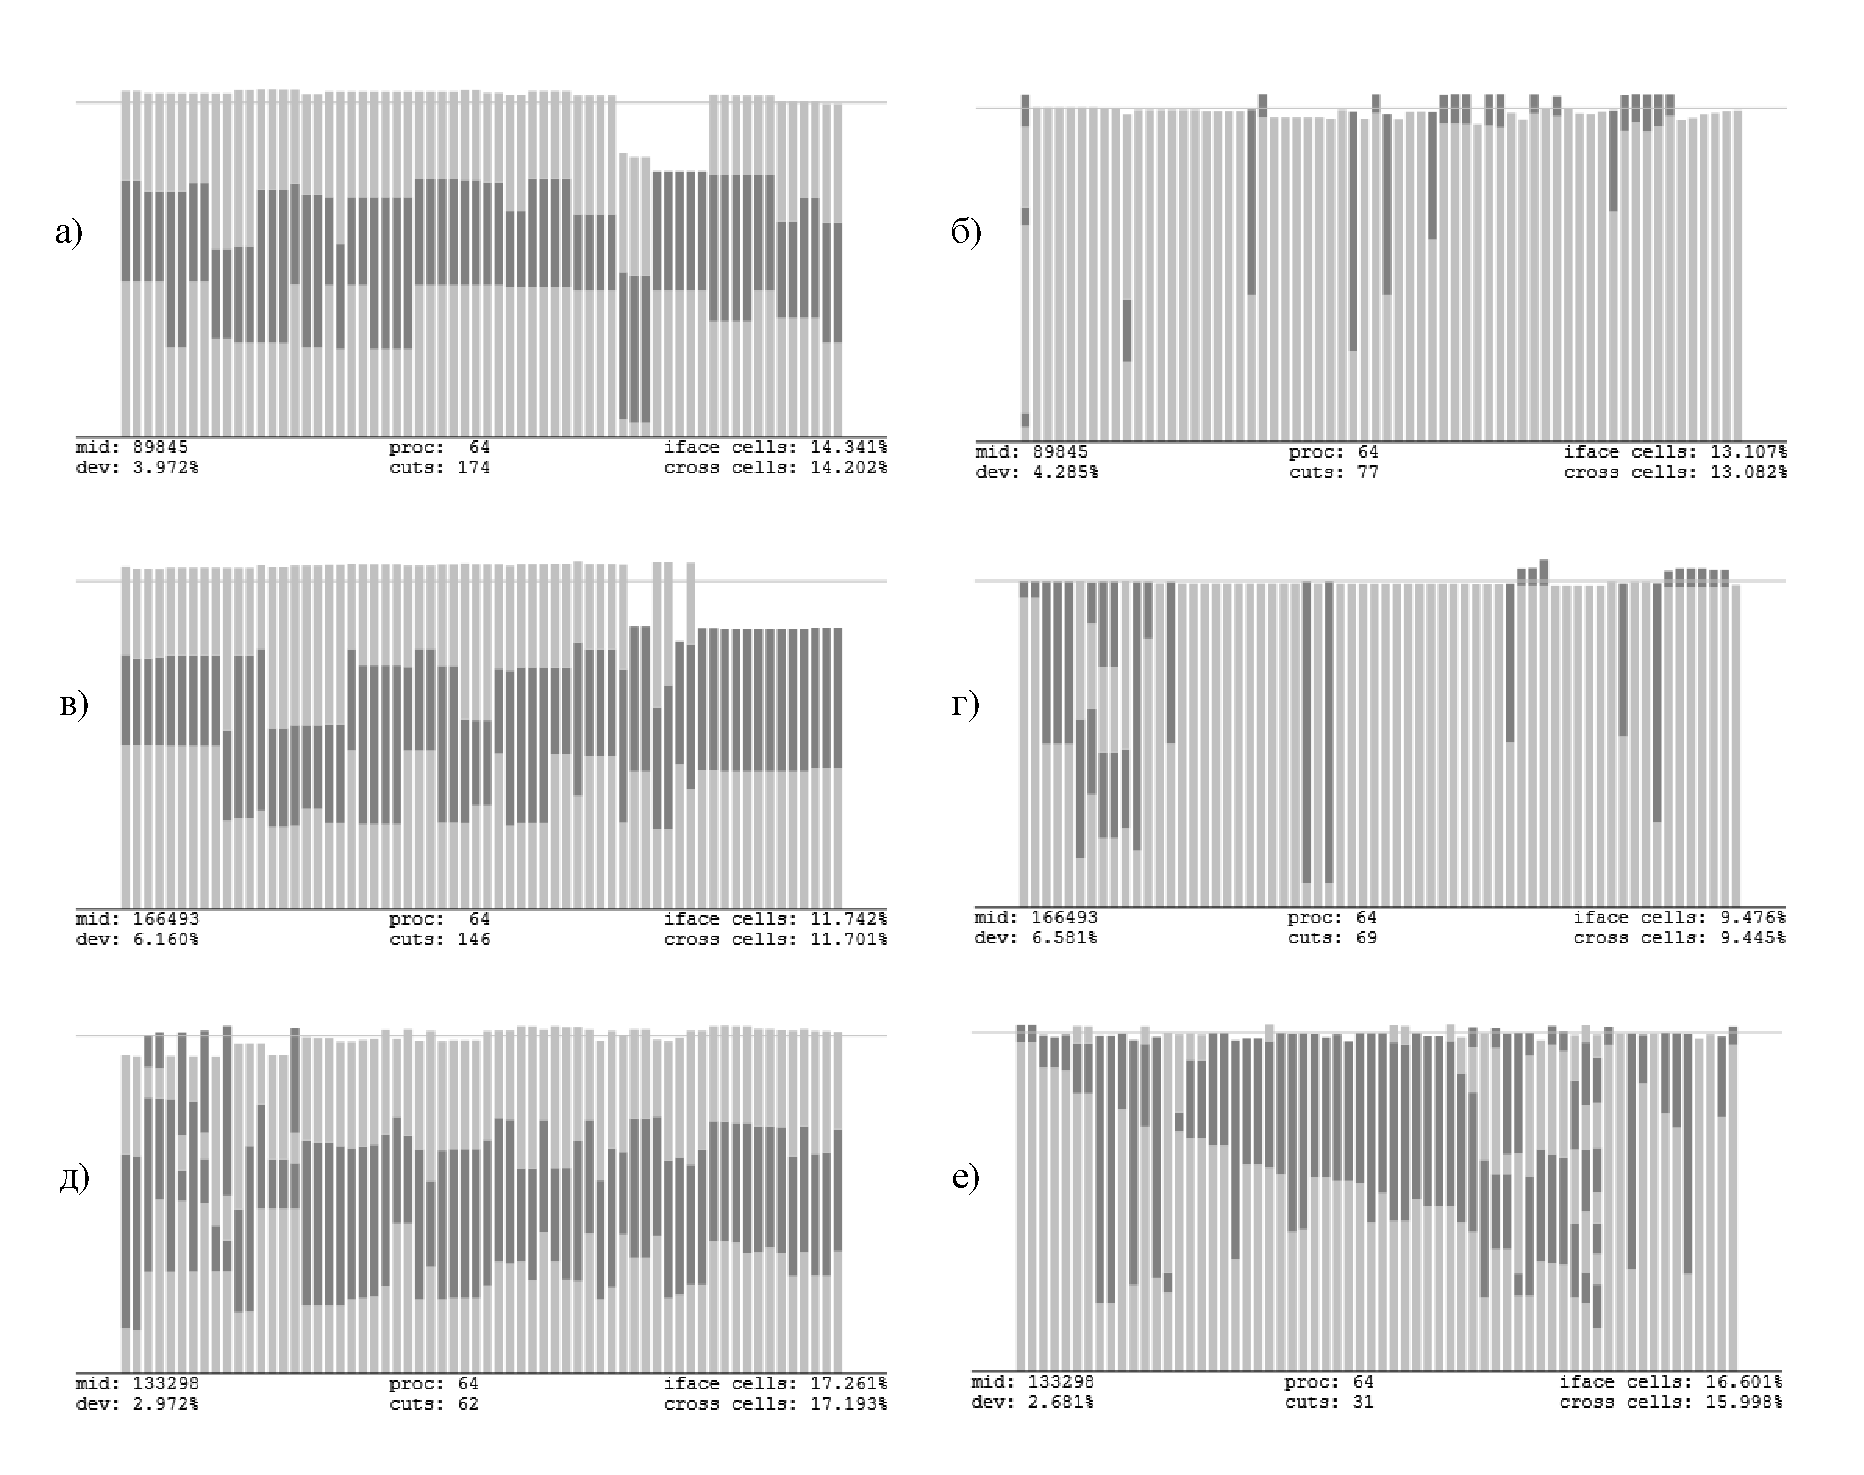
\includegraphics[width=1.0\textwidth]{./pics/text_2_withcut/2-merged-pic.pdf}
\singlespacing
\captionstyle{center}\caption{Гистограммы распределения блоков расчетной сетки по вычислительным узлам суперкомпьютера для сеток test (а, б), train (в, г), ref (д, е) с помощью алгоритмов UG (а, в, д) и MCC (б, г. е).}
\label{fig:text_2_withcut_2_merged_pic}
\end{figure}

3) Определить множество всех блоков, которые еще не распределены ни на один вычислительный узел.
Если это множество пусто, то алгоритм заканчивает работу.

4) Попробовать найти из рассматриваемого множества блоков такой блок, который можно распределить на один из вычислительных узлов так, чтобы вес этого узла не превысил $max$.
Если таких блоков несколько, то нужно взять такой блок, который максимально приближает вес соответствующего вычислительного узла к отметке $max$.
Если это удалось сделать, то распределить найденный блок на вычислительный узел и перейти к пункту 3.

5) Определить множество допустимых разрезов всех нераспределенных на текущий момент блоков.
Каждый потенциальный разрез делит блок на две части.
Определить множество таких потенциальных результирующих блоков и из этих потенциальных блоков выбрать блок веса $w$ и вычислительный узел веса $W$ такие, что $W + w \le max$ и величина $max - (W + w)$ минимальна.
Если такой пары блок-узел не найдено, то найти такую пару, что $W + w > max$ и величина $(W + w) - max$ минимальна.
Такая пара найдется всегда.
После этого выполнить необходимый разрез для получения найденного блока и распределить его на соответствующий вычислительный узел, после чего перейти к пункту 2.

Результаты сравнения эффективности методов UG и MCC распределения вычислительной нагрузки между узлами суперкомпьютера показывают, что использование метода MCC оправдано, так как с его помощью можно добиться распределения не худшего качества (а зачастую и лучшего), чем при использовании UG.
При этом MCC позволяет существенно сократить количество разрезов блоков сетки для достижения требуемого результата.
Также использование MCC приводит к сокращению количества MPI ячеек в сетке, что положительно сказывается на скорости межпроцессных обменов данными.
Особенно явно достоинства метода MCC проявляются на сетках с относительно небольшим количеством блоков и наличием ярко выраженных крупных блоков.

Приводятся результаты эксперимента по выполнению расчетов на блочно-структурированной расчетной сетке с дроблением максимального блока для достижения различных значений допустимой неравномерности распределения $D^{\%}$.

\begin{figure}[ht]
\centering
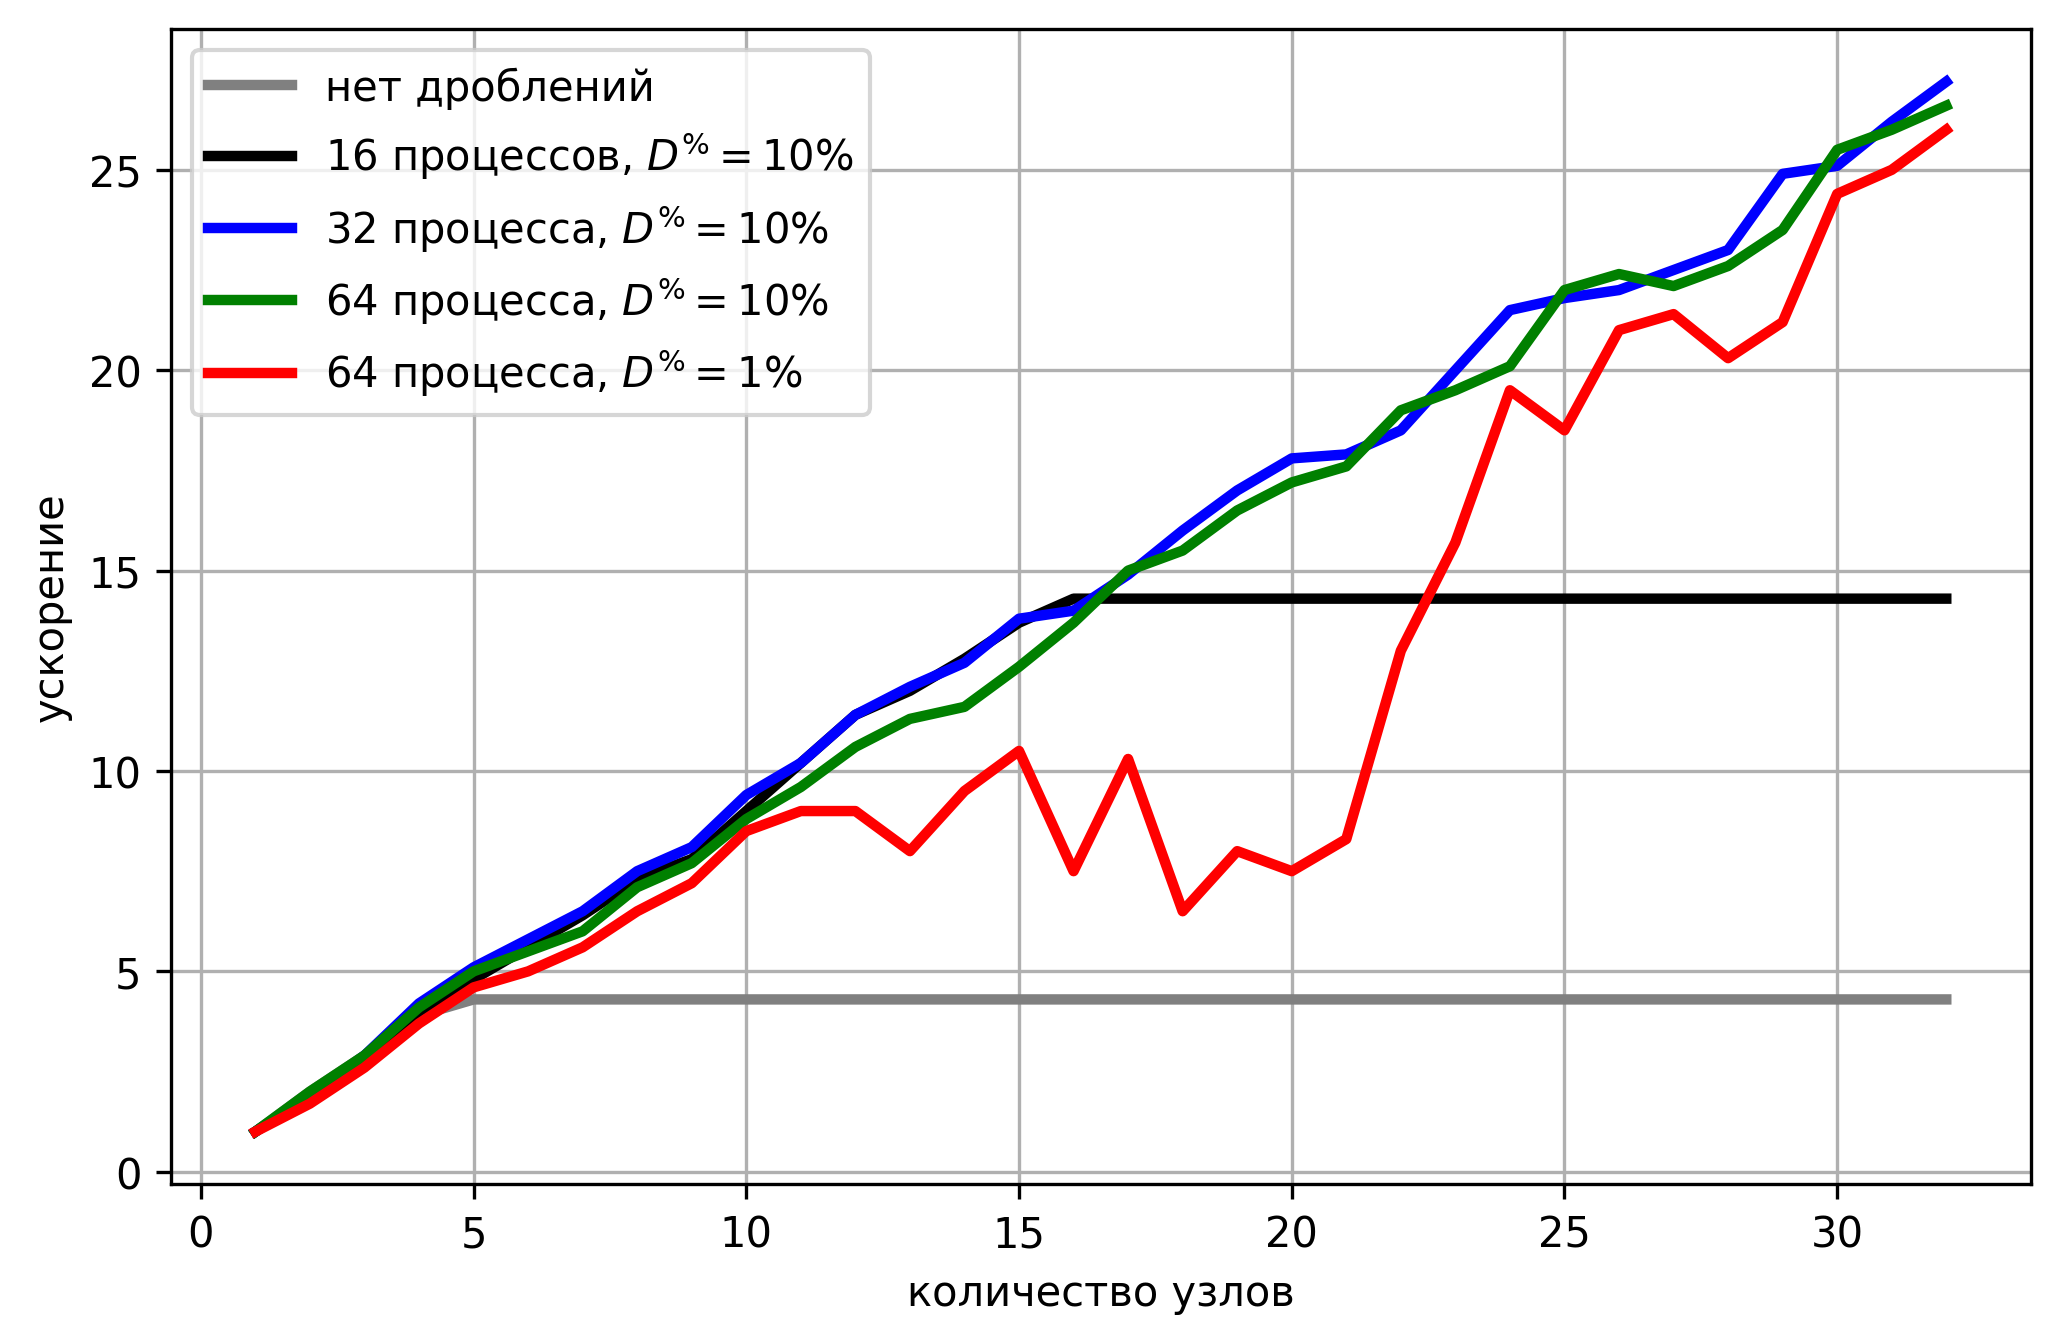
\includegraphics[width=1.0\textwidth]{./pics/text_2_withcut/scaling3.png}
\singlespacing
\captionstyle{center}\caption{Масштабирование вычислений при различных параметрах дробления сетки на 1-32 микропроцессорах Intel Xeon Phi Knights Landing 7290.}
\label{fig:text_2_withcut_scaling3}
\end{figure}

На рис.~\ref{fig:text_2_withcut_scaling3} представлены результаты численных экспериментов на сегменте суперкомпьютера, состоящем из узлов, каждый из которых содержит по одному микропроцессору Intel Xeon Phi Knights Landing 7290.
При проведении расчетов на каждом узле запускался один MPI процесс.
Количество узлов менялось от 1 до 32.
Проанализируем графики ускорения вычислений, представленные на рис.~\ref{fig:text_2_withcut_scaling3}.

Для вычислений на неподготовленной сетке (соответствует графику "нет дроблений") наблюдается ускорение для количества процессов до 5.
Далее ускорение остается на одной и той же отметке (около 4,3) и не меняется при дальнейшем увеличении количества узлов.
Это связано с наличием крупного блока, который мешает равномерному распределению вычислительной нагрузки.

При подготовке сетки для выполнения на 16 процессах (черный график) ускорение также останавливается, но на более высокой отметке (в районе 14,0).
Это также связано с наличием крупного блока, но его размер меньше, чем в случае отказа от дроблений (наиболее крупный блок был раздроблен, что привело к эффективному распределению вычислительной нагрузки для 16 процессов, однако для большего количества процессов размер этого блока препятствует равномерному распределению блоков по процессам).

При подготовке сетки для выполнения на 32 и 64 процессах с допустимым отклонением $D^{\%} = 10\%$ (синий и зеленый графики соответственно) получаем примерно одинаковое возрастание ускорения вычислений с ростом количества узлов.
Это говорит о том, что при подготовка сетки для большего количества процессов, чем реально будет использоваться для запусков, избыточно.

При подготовке сетки для выполнения на 64 процессах с допустимым отклонением $D^{\%} = 1\%$ (красный график) наблюдается сильная просадка по ускорению при использовании количества узлов от 10 до 25.
Это связано с сильным возрастанием количества дроблений, что приводит к увеличению доли межпроцессных обменов.

%----------------------------------

В п.~2.5 рассматриваются вопросы декомпозиции поверхностной неструктурированной расчетной сетки.
Отмечены два метода декомпозиции, различающиеся по показателям эффективности $D$ и $L$.
Метод декомпозиции с помощью \textit{наращивания доменов} порождает неравномерное распределение ячеек по доменам с достаточно гладкими границами.
Метод \textit{иерархического деления пополам} по наиболее протяженному геометрическому направлению наоборот порождает равномерное распределение ячеек по доменам с протяженными <<пилообразными>> границами.

%----------------------------------

В п.~2.6 рассматривается алгоритм сглаживания границ между доменами при декомпозиции поверхностной сетки.

При использовании декомпозиции расчетной сетки основным показателем качества декомпозиции является параметр $D$, так как он отражает равномерность распределения ячеек по разным вычислительным процессам.
Однако если игнорировать остальные показатели, то в процессе декомпозиции могут появляться протяженные <<пилообразные>> границы между доменами, которые приводят к возрастанию параметров качества декомпозиции $L$ и $I$, что негативно сказывается на производительности.
Пример возникновения таких пилообразных границ можно увидеть на рис.~\ref{fig:text_2_smooth_bad_border}.

\begin{figure}[ht]
\centering
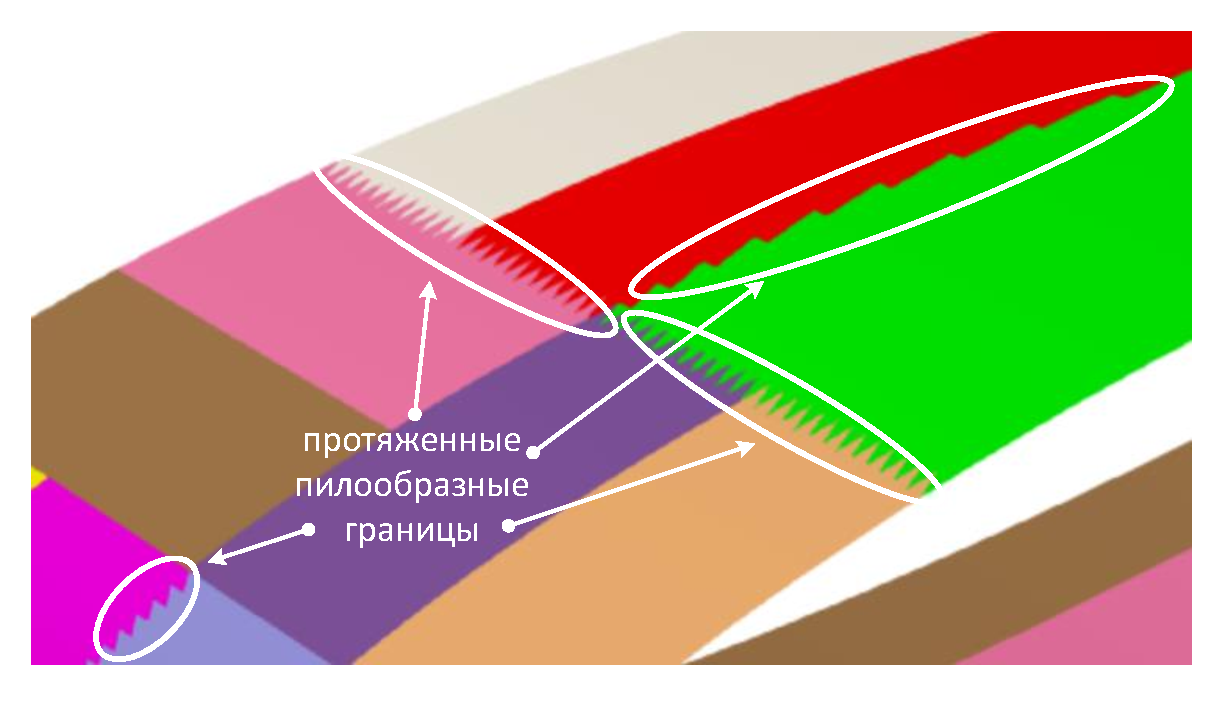
\includegraphics[width=0.6\textwidth]{./pics/text_2_smooth/bad-border.pdf}
\singlespacing
\captionstyle{center}\caption{Возникновение протяженных <<пилообразных>> границ между доменами.}
\label{fig:text_2_smooth_bad_border}
\end{figure}

Алгоритм сглаживания границ между доменами применяется последовательно к каждой паре доменов и направлен на уменьшение длины границы между ними с сохранением баланса количества ячеек в этих доменах.
Граница между двумя доменами может быть представлена в виде набора простых циклов и простых цепей.
При этом простой цикл может быть обработан таким же образом, как и простая цепь, с учетом совпадения первого и последнего узла этой цепи (для такого виртуального размыкания простого цикла может быть выбран произвольный узел этого цикла).
В процессе применения алгоритма сглаживания может быть выполнено виртуальное размыкание всех простых циклов, после чего все образовавшиеся цепи рассматриваются последовательно.
Без ограничения общности можно считать, что мы работаем с одной простой цепью (полученной с помощью записи всех отдельных простых цепей подряд), представляющей границу между парами доменов.

Вначале одним линейным проходом по цепи выполняется поиск всех пригодных для сглаживания границы шаблонов, представленных на рис.~\ref{fig:text_2_smooth_smooth_border}.

\begin{figure}[ht]
\centering
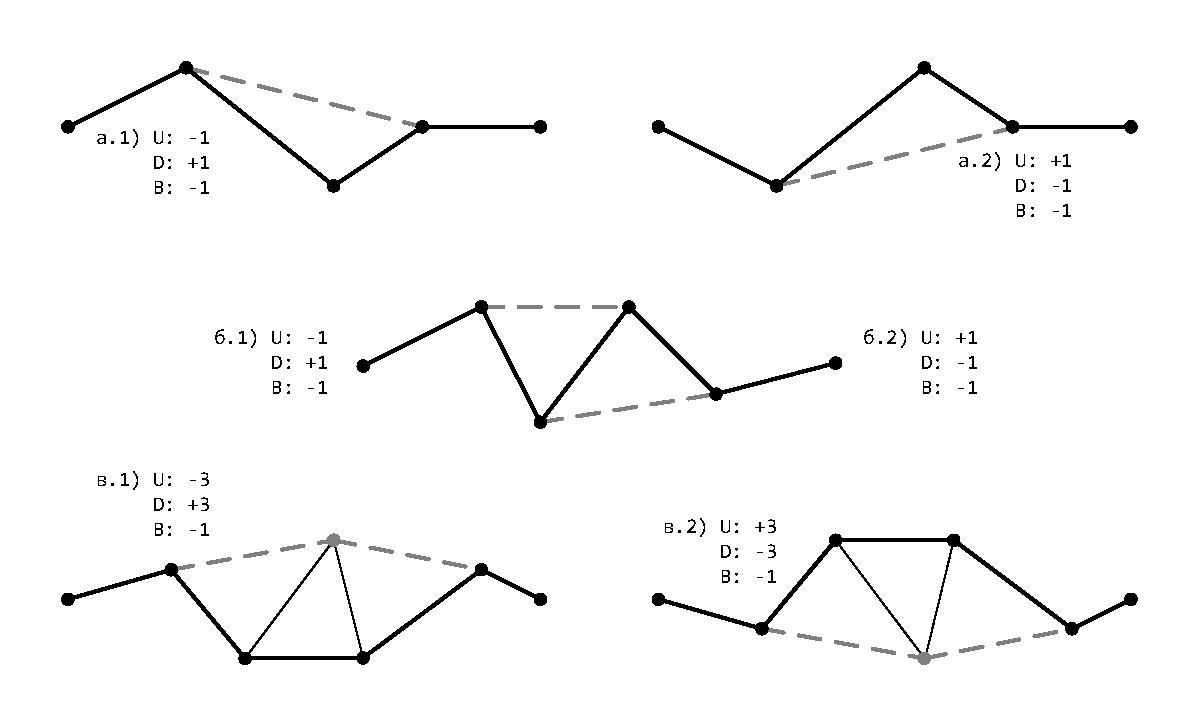
\includegraphics[width=0.8\textwidth]{./pics/text_2_smooth/smooth-border.pdf}
\singlespacing
\captionstyle{center}\caption{Шаблоны элементарных действий сглаживания границ между доменами.}
\label{fig:text_2_smooth_smooth_border}
\end{figure}

После того, как внутри цепи найдены все шаблоны, потенциально пригодные для оптимизации границы, выполняется разметка того, как данные шаблоны могут влиять на другие шаблоны.
С учетом того, что любой шаблон может повлиять только на своих непосредственных соседей, такое действие также выполняется с линейной сложностью относительно длины границы.

Последним шагом применения алгоритма является выбор такого множества шаблонов, которые не влияют друг на друга (то есть могут быть применены все одновременно) и не нарушают суммарного баланса ячеек (так как для нас важнейшим показателем эффективности декомпозиции расчетной сетки является равномерность распределения ячеек по доменам).
После выбора наибольшего возможного набора шаблонов они применяются, и на этом обработка цепи считается завершенной.

Ввиду того, что применение каждого отдельного шаблона уменьшает длину границы на 1, задача поиска оптимального решения может быть сформулирована в виде поиска в множестве шаблонов подмножества максимального размера, не содержащего конфликтующих шаблонов.
Поставленную задачу будем решать методом динамического программирования.
Для этого рассмотрим функцию $B(t, u, x)$, отражающую изменение длины границы при решении задачи на множестве шаблонов $\{ t' \in T : t' \ge t \}$ при условии изменения количества ячеек в домене $U$ на $u$ единиц.
Параметр $x$ является булевым и принимает значение $1$, если шаблон $t$ вошел в решение, и $0$ -- в противном случае.
Решением поставленной задачи является значение $\min(B(t_0, 0, 1), B(t_0, 0, 0))$, где $t_0$ -- первый шаблон на рассматриваемой цепи.

Решение задачи начинается с последнего шаблона $t_n$.
Для него все множество используемых шаблонов состоит только из него самого, и
\begin{equation}
	\left\{
		\begin{aligned}
			& B(t_n, 0, 0) = 0 \\
			& B(t_n, U(t_n), 1) = -1
		\end{aligned}
	\right.
\end{equation}
для всех остальных значений $u$ значение функции $B(t_n, u, x)$ не определено, будем считать его равным $+\infty$ (это означает, что на последнем шаблоне кроме значений $0$ и $U(t_n)$ недостижимы другие значения изменения количества ячеек в домене $U$).

Пусть задача решена для некоторого шаблона $t_{k + 1}$.
Рассмотрим переход к решению для $t_k$.
Изначально все значения $B(t_k, u, x)$ принимаются равными $+\infty$.

Во-первых, имея любое допустимое решение для шаблона $t_{k + 1}$ мы можем получить решение для шаблона $t_k$, просто проигнорировав этот шаблон, то есть для всех $u$, для которых найдено решение для шаблона $t_{k + 1}$:
\begin{equation}
	B(t_k, u, 0) = \min \left( B(t_{k + 1}, u, 0), B(t_{k + 1}, u, 1) \right)
\end{equation}

Игнорирование шаблона $t_k$ не меняет баланс ячеек между доменами.

Второй момент связан с попыткой использования шаблона $t_k$.
Если $t_k \cap t_{k + 1} = \emptyset$, то есть конфликта нет, то шаблон $t_k$ можно использовать вне зависимости от того, был ли использован шаблон $t_{k + 1}$.
То есть для всех $u$, для которых было найдено решение для шаблона $t_{k + 1}$ выполним следующее действие:
\begin{equation}
	B(t_k, u + U(t_k), 1) = B(t_k, u, 0) - 1
\end{equation}

И наконец в случае конфликтующих $t_k$ и $t_{k + 1}$ мы можем использовать шаблон $t_k$ только в том случае, если не был использован шаблон $t_{k + 1}$, то есть для всех $u$ для которых $B(t_{k + 1}, u, 0) \ne +\infty$ нужно выполнить операцию
\begin{equation}
	B(t_k, u + U(t_k), 1) = B(t_{k + 1}, u, 0) - 1
\end{equation}

В результате работы алгоритма рассчитываются оптимальные решения для всех значений $u$ из диапазона
\begin{equation}
	[U_{min}, U_{max}] = \left[ \frac{1}{2} \sum_{t \in T}{(U(t) - |U(t)|)}, \frac{1}{2} \sum_{t \in T}{(U(t) + |U(t)|)} \right]
\end{equation}

и его сложность равна $O \left( |T| \cdot (U_{max} - U_{min} + 1) \right)$.

\begin{figure}[!ht]
\centering
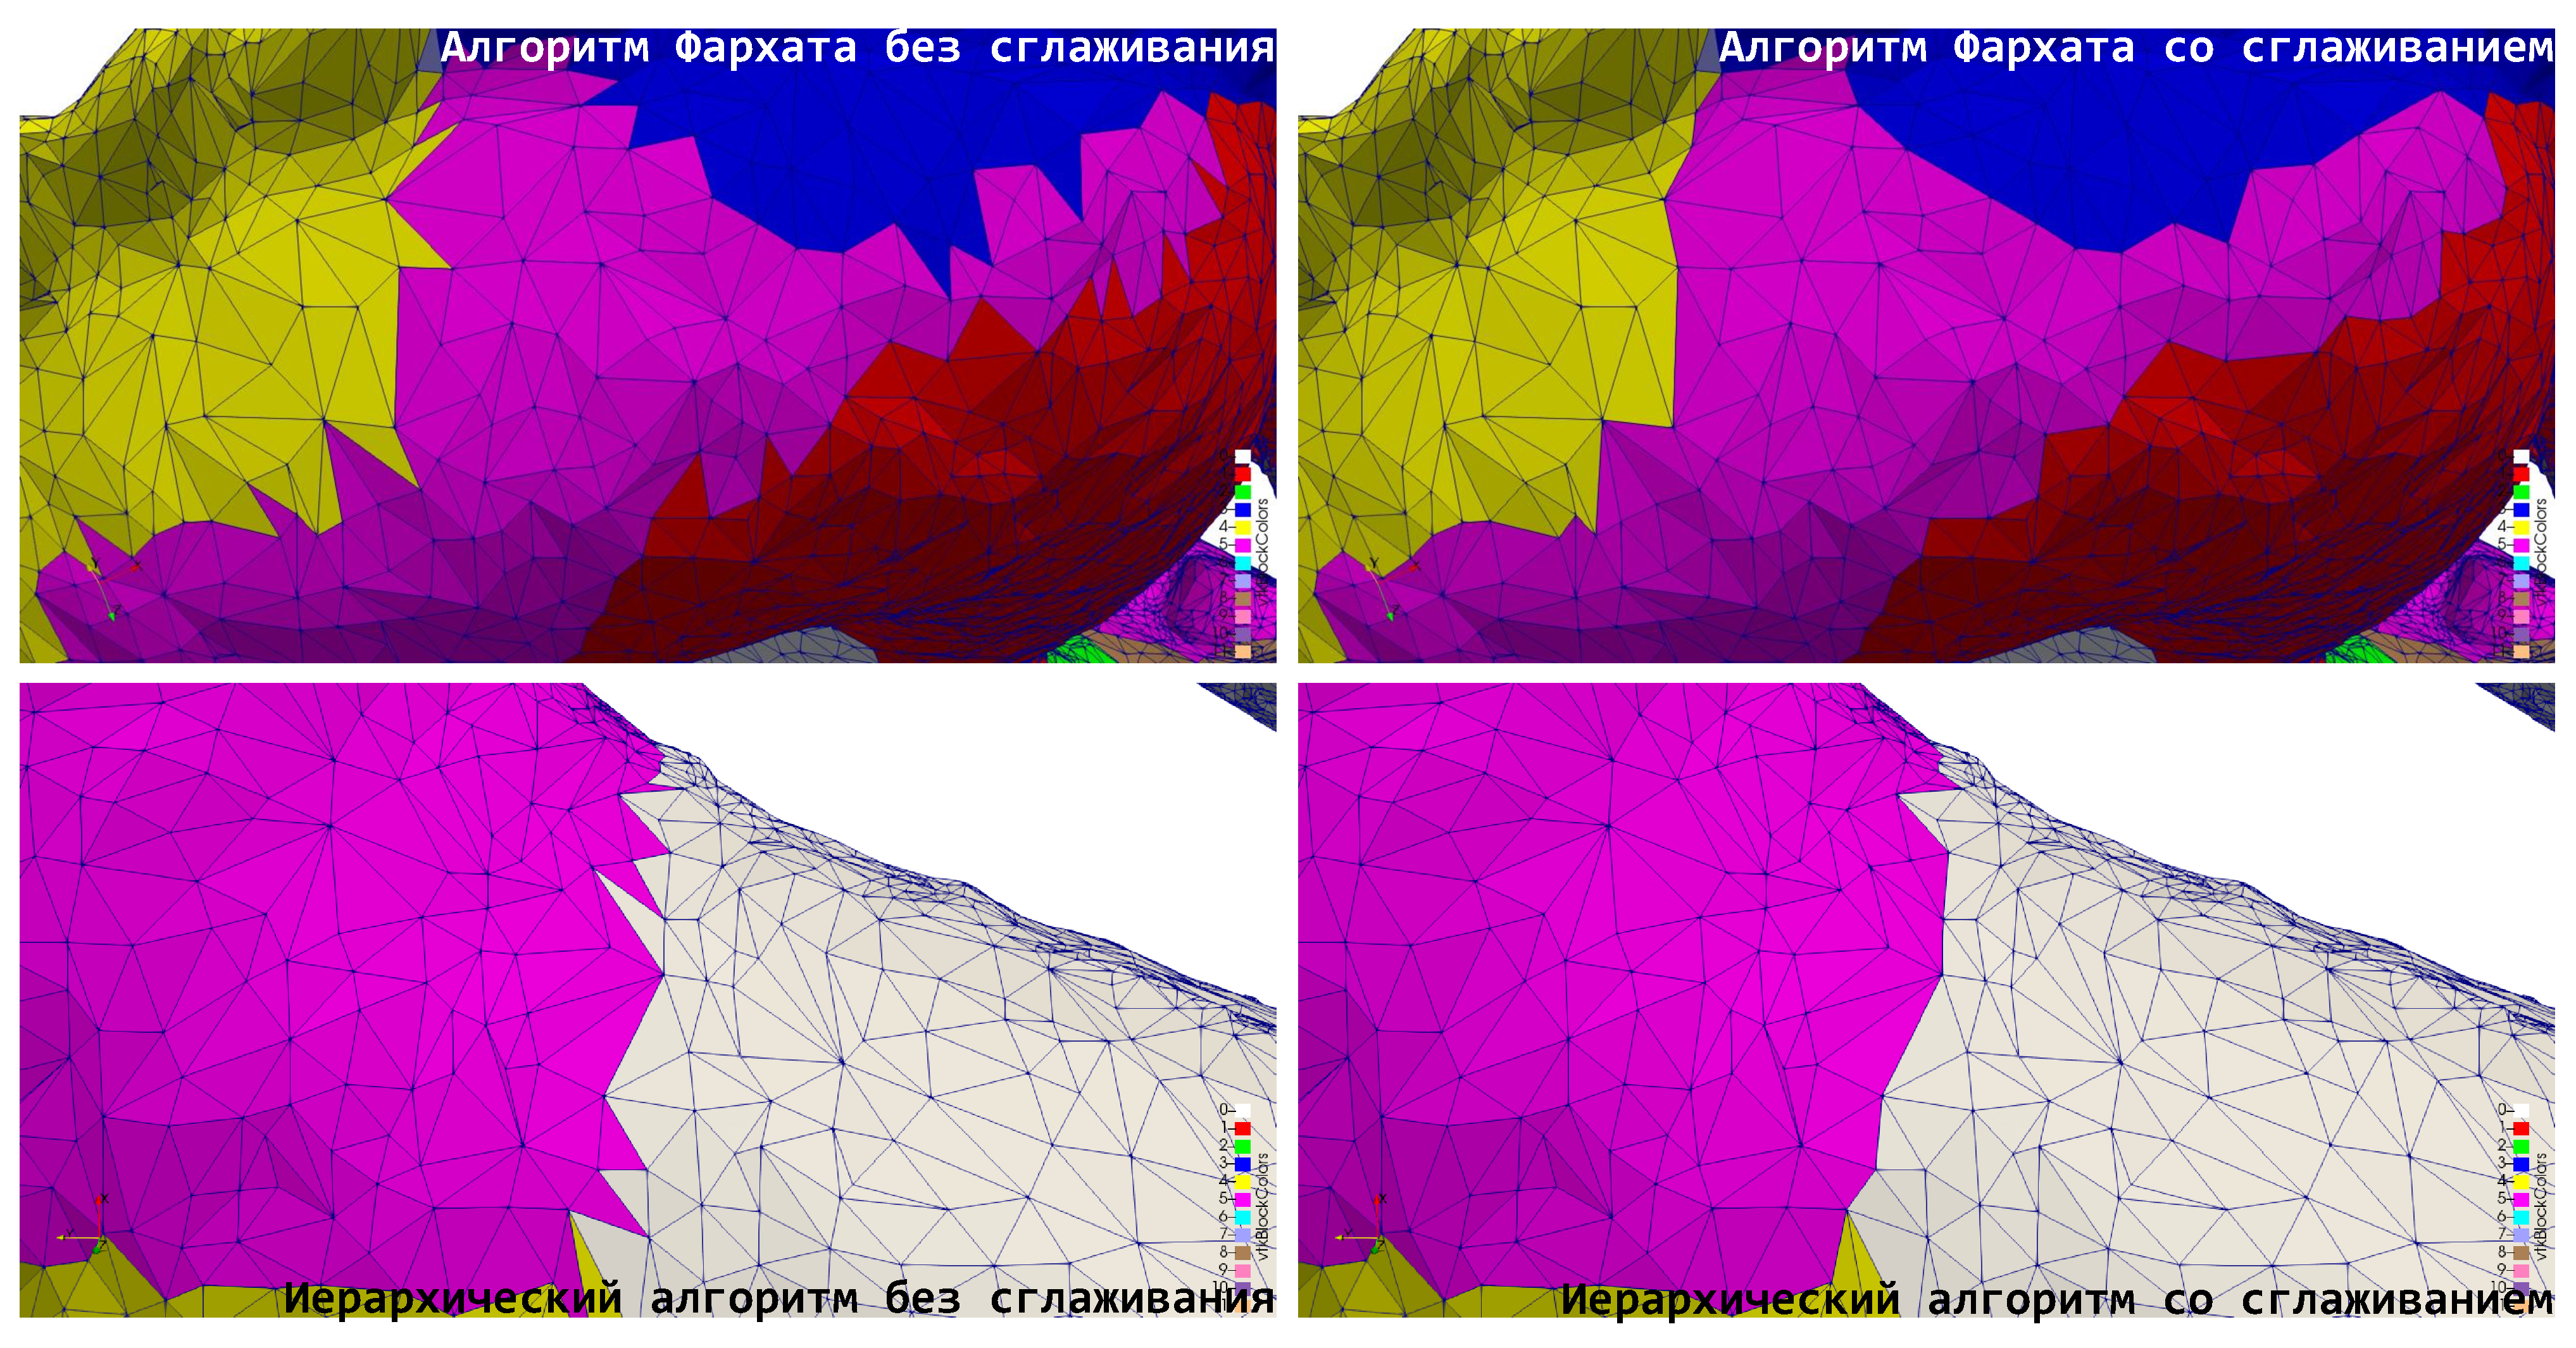
\includegraphics[width=0.8\textwidth]{./pics/text_2_smooth/decomp2.pdf}
\singlespacing
\captionstyle{center}\caption{Визуализация применения сглаживания границ между доменами после работы алгоритма Фархата (сверху) и иерархического алгоритма (снизу).}
\label{fig:text_2_smooth_decomp2}
\end{figure}

На рис.~\ref{fig:text_2_smooth_decomp2} крупным планом продемонстрированы отдельные части тестовой расчетной сетки с отображением ребер ячеек.
На этом рисунке виден эффект от применения алгоритма сглаживания границ между доменами, прежде всего от заключается в устранении одиноких ячеек, которые вторгаются в соседний домен одной своей вершиной.
После применения алгоритма границы между доменами визуально выглядят более гладко, их длина уменьшается.
Применение алгоритма сглаживания границ приводит к сокращению как общего количества граничных ребер, так и длины максимальной границы примерно на 10\%.

%----------------------------------

В п.~2.7 рассматривается применение генетического алгоритма для корректировки инициирующих вершин при использовании алгоритма декомпозиции графа с помощью наращивания доменов.

Ключевым элементом генетического алгоритма является понятие генотипа и процесс формирования особи на основе генотипа.
В качестве генотипа будем использовать вектор \texttt{genotype} длины $k$, задающий $k$ номеров вершин дуального графа, которые будем называть опорными вершинами.
При инициализации каждую опорную вершину \texttt{genotype[i]} будем принудительно относить к $i$-му домену.
При построении особи на основе генотипа будем распределять вершины между доменами с помощью простого алгоритма, схожего с алгоритмом пузырькового роста, начиная с опорных вершин и обходя граф в ширину.

В результате применения генетического алгоритма значение штрафной функции лучшей особи за время работы алгоритма падает примерно на 50-75\%, если считать от значения лучшей особи стартовой популяции.

%---------------------------------------------------------------------------------------------------

\begin{figure}[!ht]
\centering
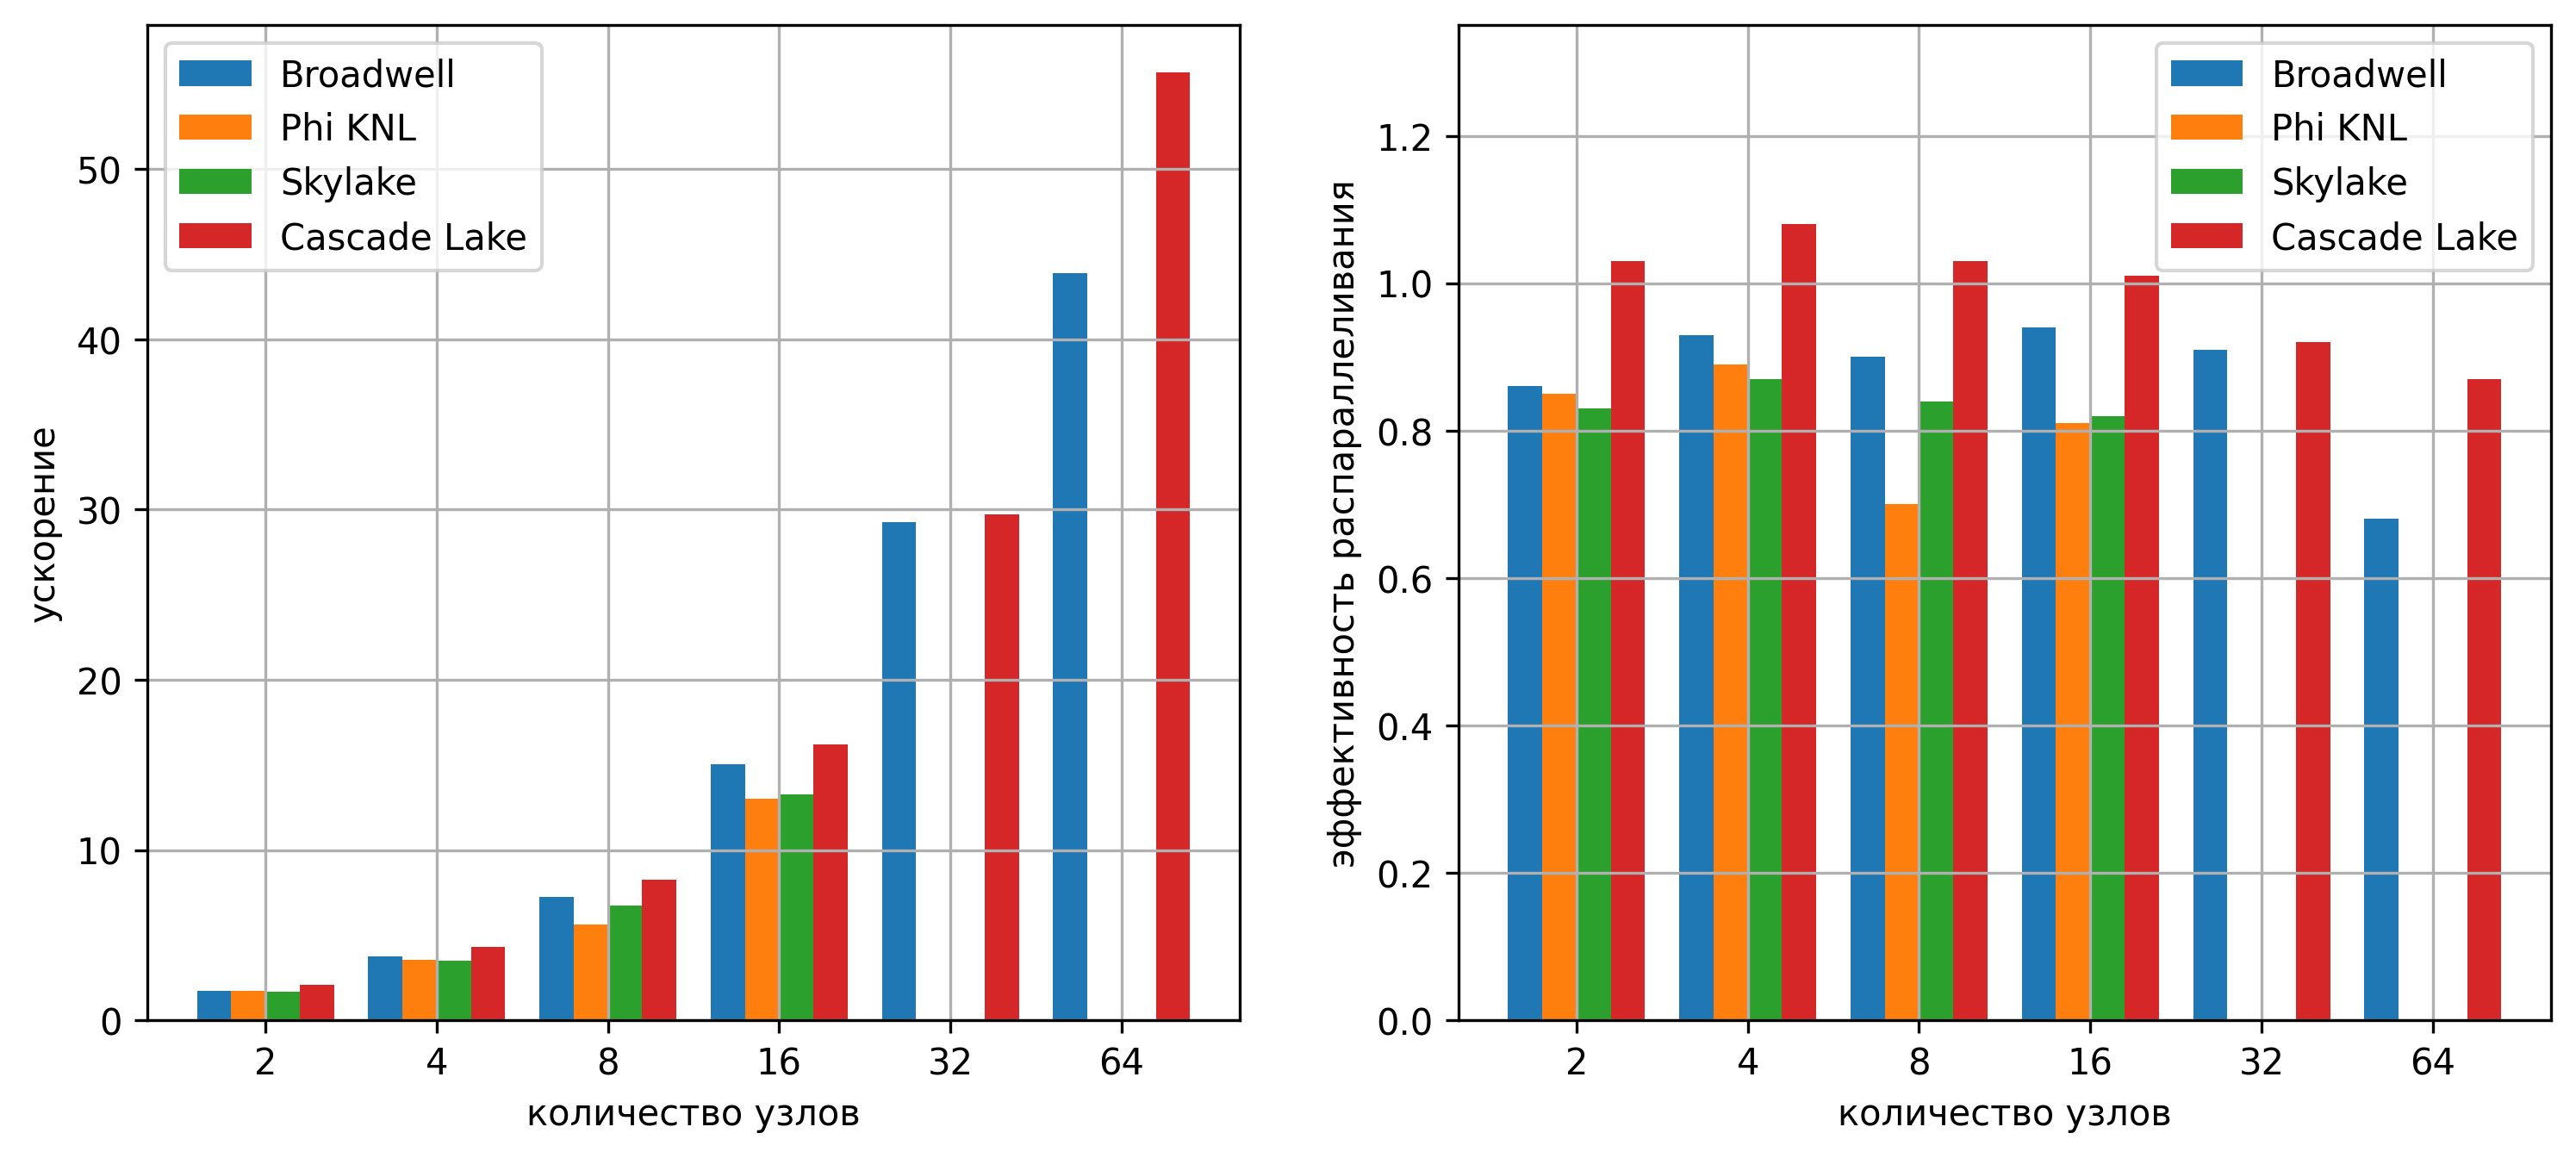
\includegraphics[width=1.0\textwidth]{pics/text_2_scaling/2in1.png}
\singlespacing
\captionstyle{center}\caption{Ускорение (слева) и эффективность распараллеливания (справа) вычислений на сегментах суперкомпьютера МВС-10П при увеличении количества узлов.}
\label{fig:text_2_scaling_speedup_eff}
\end{figure}

В п.~2.8 приводится описание эксперимента по замеру ускорения и эффективности распараллеливания задачи расчета ледообразования на поверхностной неструктурированной расчетной сетки с использованием иерархической геометрической декомпозиции сетки со сглаживанием границ между доменами. Замеры производились на вычислительных сегментах суперкомпьютера МВС-10П на базе микропроцессоров Intel разных поколений.
Результаты эксперимента показали, что достигается высокая эффективность распараллеливания вычислений на всех сегментах при использовании до 64 вычислительных узлов (рис.~\ref{fig:text_2_scaling_speedup_eff}).

%---------------------------------------------------------------------------------------------------

\textbf{Четвертая глава} посвящена проблемам векторизации программного кода.
Отмечается, что векторизация является низкоуровневой оптимизацией распараллеливания вычислений на уровне отдельных инструкций, векторные инструкции поддержаны во всех современных микропроцессорных архитектурах (x86, ARM, Power, <<Эльбрус>>, LoongArch, Sunway и других), и правильное применение векторизации способно кратно увеличить производительность приложений.
Выделяется набор инструкций AVX-512, как поддерживающий возможность выборочной обработки элементов векторов, что делает возможным векторизацию сложного программного контекста с обилием операций передачи управления, гнездами циклов и вызовами функций.
Отмечается проблема недостаточно эффективного применения векторизации оптимизирующим компилятором для сложного программного контекста.
Для оценки применения векторизации используются понятия \textit{ширина векторизации} $w = \frac{v}{t}$ (где $v$ -- размер векторного регистра, $t$ -- размер типа расчетных данных), \textit{ускорение от применения векторизации} $s_{vec} = \frac{T}{T_v}$ (где $T$ -- время выполнения невекторизованной версии кода, $T_v$ -- время выполнения векторизованной версии кода), \textit{эффективность векторизации} $e_{vec} = \frac{s_{vec}}{w}$.

%----------------------------------

В п.~4.1 приведено описание набора векторных инструкций AVX-512, перечислены основные подмножества операций и рассмотрены особенности этого набора.
В качестве основной отличительной черты набора инструкций AVX-512, позволяющей векторизовать программный контекст со сложным управлением, названа возможность выполнения векторных инструкций с использованием \textit{векторных масок}, определяющих индексы элементов, для которых в выходной регистр записывается результат операции.

%----------------------------------

В п.~4.2 и п.~4.3 рассматривается векторизация программного кода путем выделения однотипных операций и объединения их в векторные аналоги на примере операций с матрицами малой размерности.
На примере матричных операций показано, что от способа выделения однотипных операций для объединения в векторные аналоги существенным образом зависит производительность результирующего кода.
Также продемонстрировано, что низкая плотность векторных масок в результирующем коде негативно сказывается на производительность.

%----------------------------------

В п.~4.4 вводится понятие \textit{плоского цикла} как удобного контекста для векторизации вычислений, что делает его предпочтительной формой компоновки программного кода для успешного автоматического применения векторизации оптимизирующим компилятором.

\begin{figure}[ht]
\centering
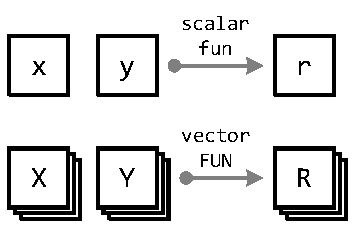
\includegraphics[width=0.4\textwidth]{./pics/text_4_flat/fun.pdf}
\singlespacing
\captionstyle{center}\caption{Схема выполнения скалярной функции fun и аналогичной векторной функции FUN.}
\label{fig:text_4_vec_flat_fun_FUN}
\end{figure}

Основная идея плоского цикла состоит в объединении нескольких вызовов (в количестве, равном ширине векторизации $w$) скалярной функции в единую векторную реализацию (рис.~\ref{fig:text_4_vec_flat_fun_FUN}).
Здесь $w$ экземпляров функции $fun(x, y) \rightarrow r$ со скалярными параметрами $x$, $y$ и скалярным результатом $r$ объединены в функцию $FUN(X, Y) \rightarrow R$ с векторными параметрами $X$, $Y$ и векторным результатом $R$.

\begin{table}[!ht]
\centering
\singlespacing
\captionstyle{center}\caption{Инструкции AVX-512 для работы с вещественными числами \\ и их семантика.}
\bigskip
\label{tbl:text_4_flat_avx512semantic}
\begin{tabular}{ | c | c | }
  \hline
  Имя инструкции & Семантика инструкции \\ \hline\hline
  \makecell{VMOVAPS, VMOVUPS, VSQRTPS, \\ VGETEXPPS, VGETMANTPS, \\ VRCP14PS, VREDUCEPS, VRNDSCALEPS, \\ VRSQRT14PS, VSCALEFPS} & $\begin{matrix} R = op \ A \\ R = \check{P} \ ? \ (op \ A) : R \\ R = \check{P} \ ? \ (op \ A) : 0 \end{matrix}$ \\ \hline
  \makecell{VADDPS, VANDPS, VANDNPS, VDIVPS, \\ VMAXPS, VMINPS, VMULPS, VORPS, \\ VSUBPS, VRANGEPS} & $\begin{matrix} R = op \ A, B \\ R = \check{P} \ ? \ (op \ A, B) : R \\ R = \check{P} \ ? \ (op \ A, B) : 0 \end{matrix}$ \\ \hline
  \makecell{VFMADD*PS, VFMSUB*PS, \\ VFNMADD*PS, VFNMSUB*PS} & $\begin{matrix} R = op \ R, A, B \\ R = \check{P} \ ? \ (op \ R, A, B) : R \\ R = \check{P} \ ? \ (op \ R, A, B) : 0 \end{matrix}$ \\ \hline
  \makecell{VCMPPS} & $\begin{matrix} \check{P} = op \ A, B \\ \check{P} = \check{Q} \ ? \ (op \ A, B) : 0 \end{matrix}$ \\ \hline
  \makecell{VBLENDPS} & $\begin{matrix} R = \check{P} \ ? \ A : B \end{matrix}$ \\ \hline
\end{tabular}
\end{table}

В качестве плоского цикла рассматривается цикл \texttt{for}, в котором индуктивная переменная $i$ последовательно принимает значения от $0$ до $w - 1$ (\texttt{for (int i = 0; i < w; ++i)}).
К плоскому циклу предъявляются следующие требования.
На $i$-ой итерации все обращения к данным на запись имеют вид \texttt{a[i]}, а обращения к данным на чтение либо имеют вид \texttt{a[i]}, либо являются чтением скаляров.
Все массивы данных, обращение к которым на $i$-ой итерации цикла имеет вид \texttt{a[i]}, выровнены в памяти на размер вектора.
В цикле отсутствуют межитерационные зависимости.

Программный контекст, удовлетворяющий требованиям, предъявляемым к плоским циклам, является удобным для векторизации, а логика работы многих векторных инструкций может быть представлены в виде плоского цикла и записана в предикатной форме, как это показано в таблице~\ref{tbl:text_4_flat_avx512semantic}.

%----------------------------------

В п.~4.5 обсуждается применение автоматической векторизации к программному коду, представленному в виде композиции плоских циклов, а также демонстрируется негативное влияние, оказываемое отклонением от требований плоского цикла на производительность результирующего кода.
В качестве программного контекста рассматривается реализация газодинамического решателя с использованием метода погруженной границы для аппроксимации граничных условий.

Для приведения программного кода к виду плоских циклов применяется организация данных в виде набора массивов, а также расщепление циклов по константному условию для сокращения количества операций передачи управления внутри цикла.

\begin{figure}[ht]
\centering
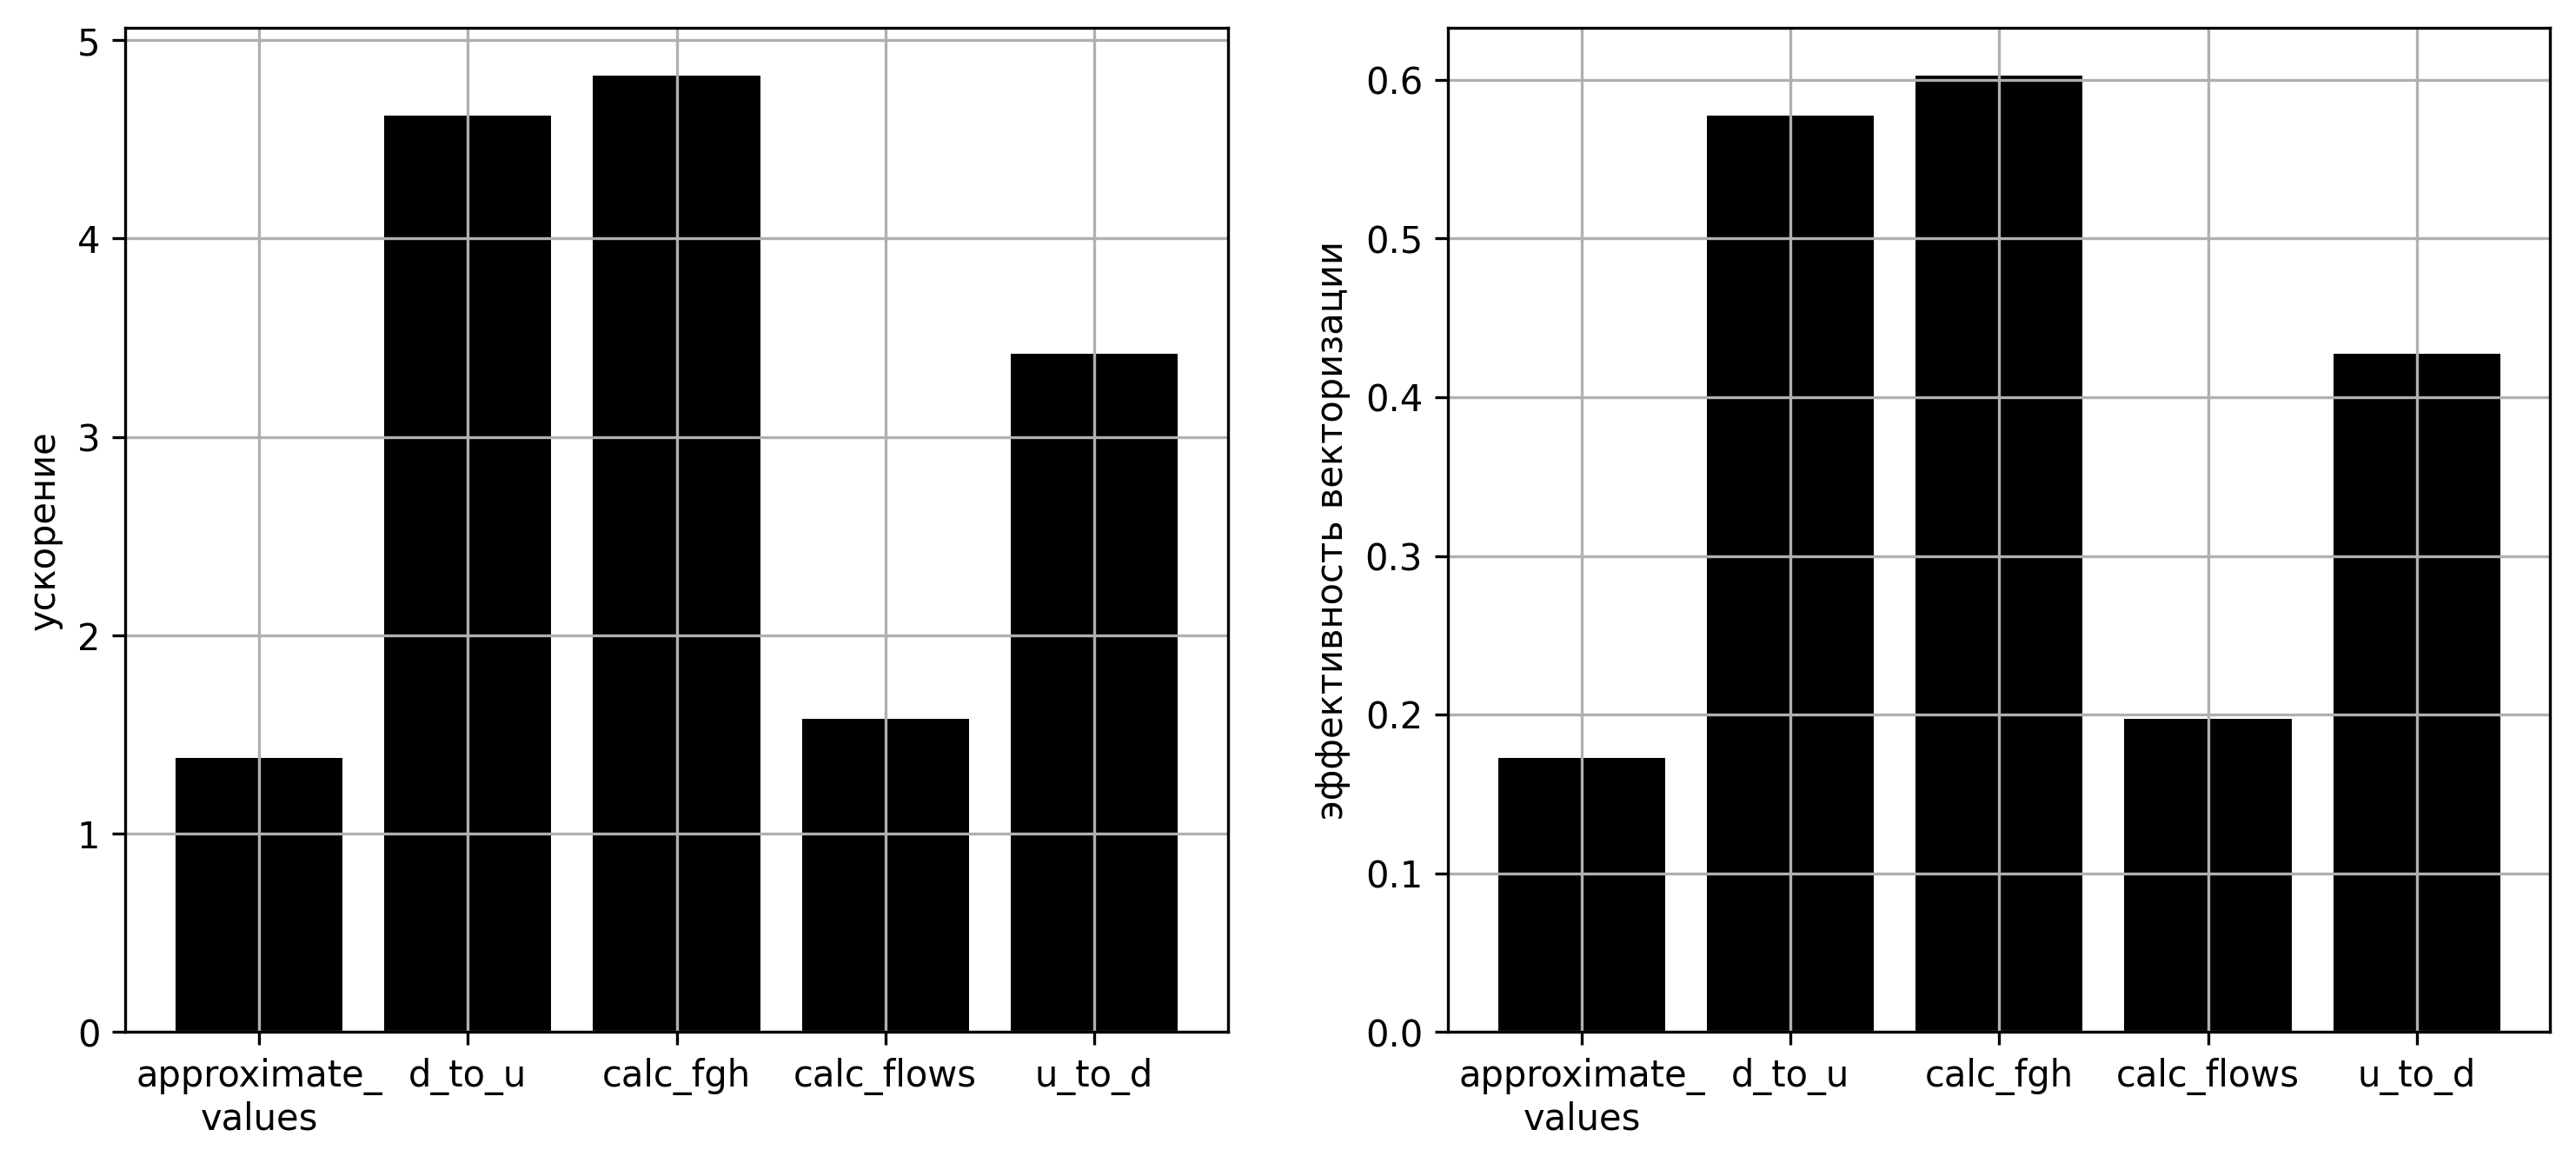
\includegraphics[width=0.6\textwidth]{./pics/text_4_ibm/diagr2.png}
\singlespacing
\captionstyle{center}\caption{Ускорение кода и эффективность векторизации отдельных функций газодинамического решателя.}
\label{fig:text_4_ibm_diagr2}
\end{figure}

Векторизованные версии функций, удовлетворяющие требованиям плоских циклов, продемонстрировали более высокую эффективности векторизации (зеленые столбцы на рис.~\ref{fig:text_4_ibm_diagr2}).

%----------------------------------

В п.~4.6 рассматривается оптимизация выноса маловероятного региона из плоского цикла.
Оптимизация заключается в сохранении условий входа в маловероятный регион во временный массив и удалении этого региона из основного цикла.
Основной цикл, свободный от удаленного региона, может быть успешно векторизован, а вынесенный маловероятный регион может быть обработан в отдельном цикле согласно сохраненным условиям.

%----------------------------------

В п.~4.7 и п.~4.8 рассматривается процедура \textit{слияния путей исполнения по условию} внутри плоского цикла с помощью постановки операций из параллельных линейных участков под сооответствующие предикаты.

\begin{figure}[ht]
\centering
\begin{tabular}{ll}
	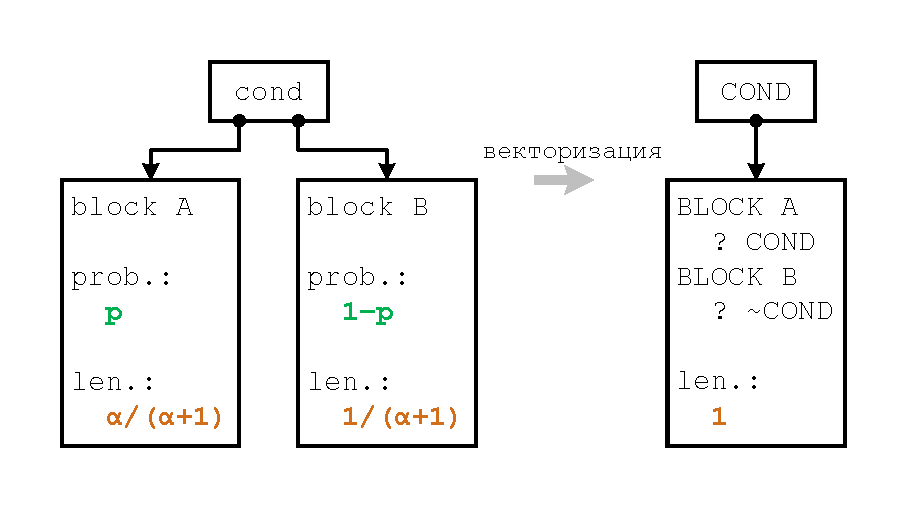
\includegraphics[width=0.45\textwidth]{./pics/text_4_vec_mrg_under_cond/cond.pdf}
	&
	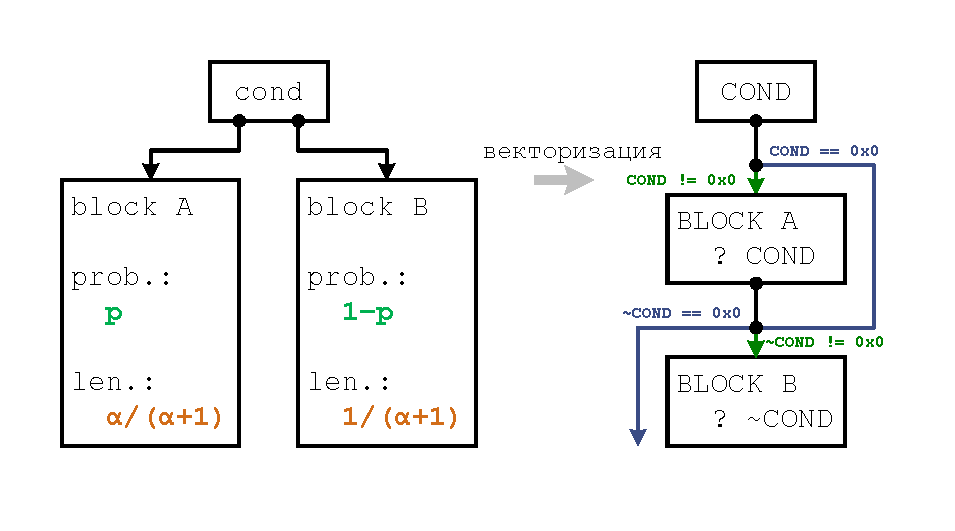
\includegraphics[width=0.45\textwidth]{./pics/text_4_vec_check_mask/cond.pdf}
\end{tabular}
\singlespacing
\captionstyle{center}\caption{Схема векторизации со слиянием двух линейных участков по условию без проверки векторной маски (слева) и с проверкой (справа).}
\label{fig:text_4_vec_mrg_under_cond_cond}
\end{figure}

Приводятся теоретические оценки эффективности векторизации плоского цикла, в котором два линейных участка сливаются по условию.
При этом рассматриваются два варианта векторного кода -- без проверки векторной маски линейного участка на пустоту перед его выполнением и с проверкой (рис.~\ref{fig:text_4_vec_mrg_under_cond_cond}).

\begin{figure}[ht]
\centering
\begin{tabular}{ll}
	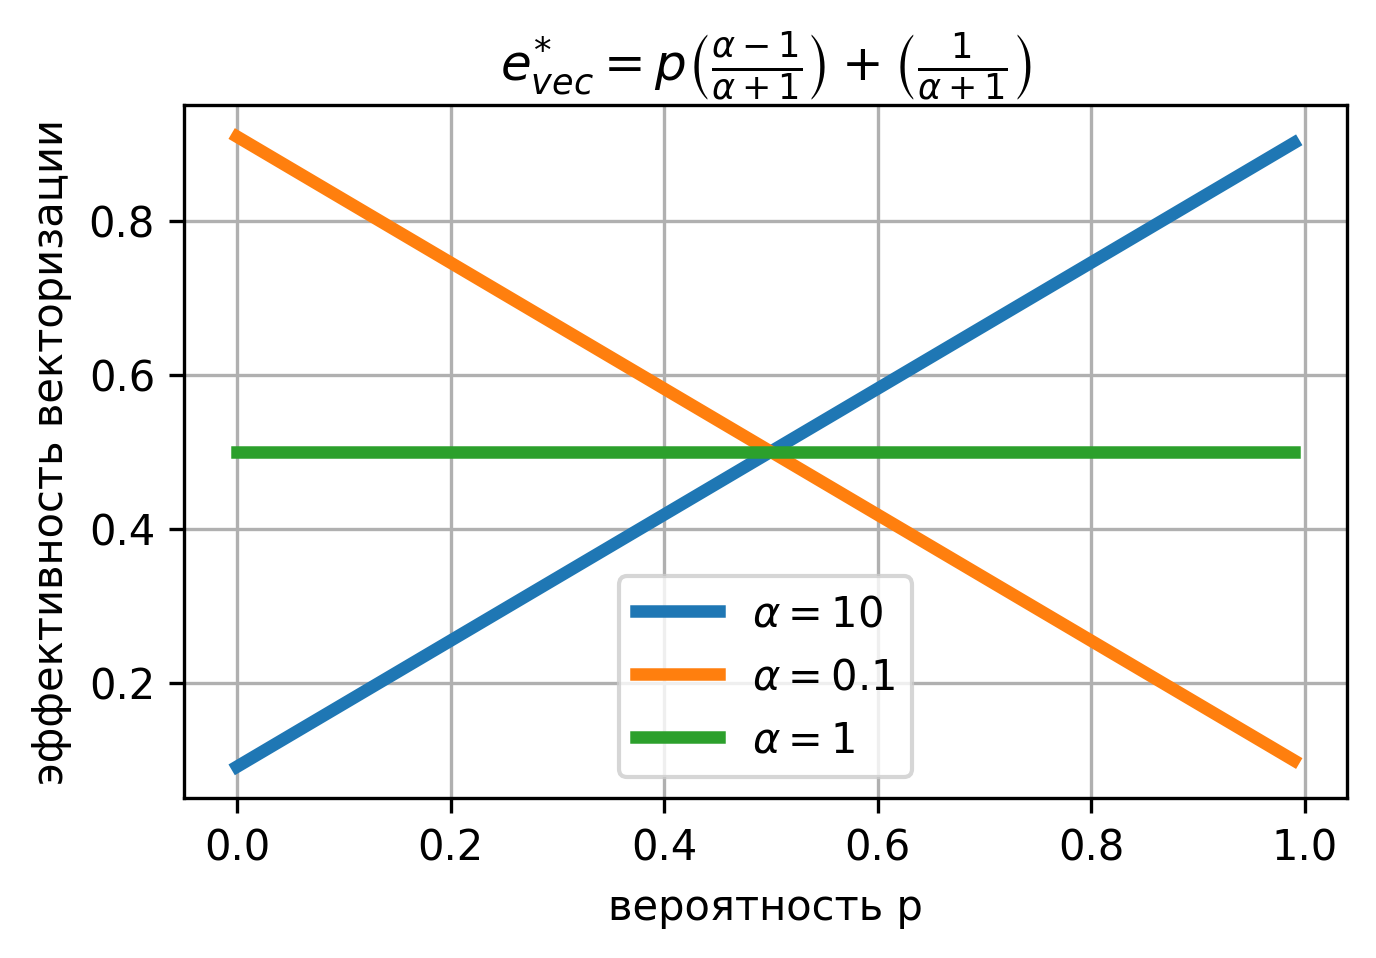
\includegraphics[width=0.45\textwidth]{./pics/text_4_vec_mrg_under_cond/chart_e_merged.png}
	&
	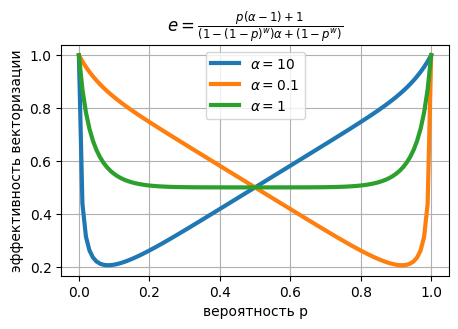
\includegraphics[width=0.45\textwidth]{./pics/text_4_vec_check_mask/chart_e_merged.png}
\end{tabular}
\singlespacing
\captionstyle{center}\caption{Графики зависимостей эффективности векторизации от вероятности перехода $p$ при значениях $\alpha = 10,0$, $\alpha = 0,1$, $\alpha = 1,0$ для слияния двух линейных участков без проверки векторной маски (слева) и с проверкой (справа).}
\label{fig:text_4_vec_under_cond_chart_e_merged}
\end{figure}

Графики зависимостей эффективности векторизаици для разных соотношений длин линейных участков приведены на рис.~\ref{fig:text_4_vec_under_cond_chart_e_merged}.
Полученные зависимости показывают низкую эффективность векторизации при слиянии большого количества путей исполнения внутри плоского цикла.

\begin{figure}[ht]
\centering
\begin{tabular}{ll}
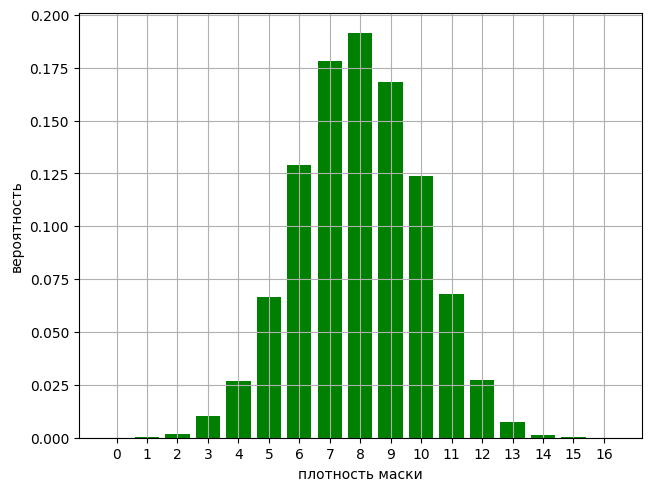
\includegraphics[width=0.45\textwidth]{./pics/text_4_vec_comb_mask/independent_p.png}
&
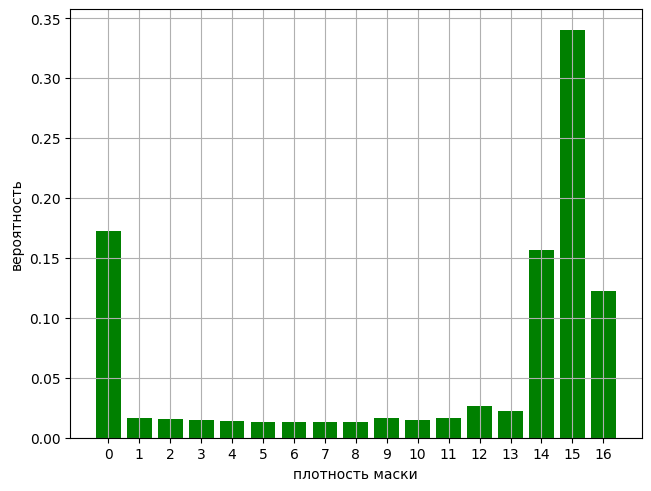
\includegraphics[width=0.45\textwidth]{./pics/text_4_vec_comb_mask/real_p.png}
\end{tabular}
\singlespacing
\captionstyle{center}\caption{Типовая гистограмма распределения плотности векторной маски в предположении независимости условия (слева) и на реальном профиле исполнения (справа).}
\label{fig:text_4_vec_comb_mask_independent_p}
\end{figure}

Отмечается, что проверка векторной маски на пустоту перед выполнением линейного участка зачастую оправдана, так как на реальных приложениях пустые и полные маски встречаются достаточно часто (рис.~\ref{fig:text_4_vec_comb_mask_independent_p}).

%----------------------------------

В п.~4.9 рассматривается подход к повышению плотности масок векторного кода с помощью \textit{объединения масок} и \textit{комбинирования масок}.
Суть объединения векторных масок заключается в следующем.
Если есть два соседних векторных блока \texttt{in\_data\_1} $\rightarrow$ \texttt{block} $\rightarrow$ \texttt{out\_data\_1} и \texttt{in\_data\_2} $\rightarrow$ \texttt{block} $\rightarrow$ \texttt{out\_data\_2}, которые должны выполняться под разными векторными масками \texttt{mask\_1} и \texttt{mask\_2}, и в дополнение к этому для этих масок выполнено условие \texttt{(mask\_1 \& mask\_2) == 0x0} (то есть маски не пересекаются), то вычисление этих двух соседних блоков можно объединить.
Вместо последовательного выполнения двух векторных блоков можно объединить входные данные \texttt{in\_data\_1} и \texttt{in\_data\_2} с помощью слияния \texttt{in\_data = blend(mask\_1, in\_data\_2, in\_data\_1}), после чего выполнить тот же блок вычислений под маской \texttt{mask\_1 | mask\_2}.
Ввиду отсутствия пересечения векторных масок в результирующих выходных данных \texttt{out\_data} будут содержаться как необходимые элементы данных \texttt{out\_data\_1}, так и необходимые элементы данных \texttt{out\_data\_2}.
Последним действием, которое нужно выполнить является извлечение из объединенного результата \texttt{out\_data} данных \texttt{out\_data\_1} и \texttt{out\_data\_2} (рис.~\ref{fig:text_4_vec_comb_mask_comb_masks}).

\begin{figure}[ht]
\centering
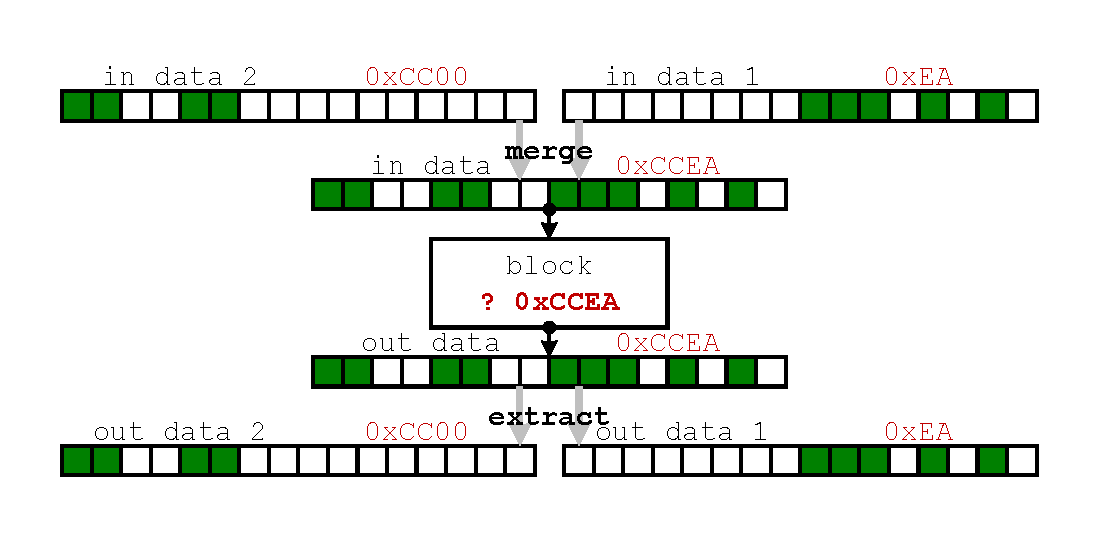
\includegraphics[width=0.8\textwidth]{./pics/text_4_vec_comb_mask/comb_masks.pdf}
\singlespacing
\captionstyle{center}\caption{Схема вычислений с объединением двух векторизованных блоков \texttt{in\_data\_1} $\rightarrow$ \texttt{block} $\rightarrow$ \texttt{out\_data\_1}, \texttt{in\_data\_2} $\rightarrow$ \texttt{block} $\rightarrow$ \texttt{out\_data\_2}}
\label{fig:text_4_vec_comb_mask_comb_masks}
\end{figure}

Комбинирование масок позволяет похожим образом объединить вычисление соседних блоков в случае пересечения векторным масок.
Комбинирование векторных масок рассматривается только теоретически, а для объединения масок поставлен эксперимент для одной из функций точного римановского решателя.
Результаты сравнения эффективнсти векторизации на эмуляторе и на реальной машине при простом слиянии путей исполнения по условию, а также с проверкой векторных масок и с объединением масок представлены на рис.~\ref{fig:text_4_vec_comb_mask_res}.

\begin{figure}[!ht]
\centering
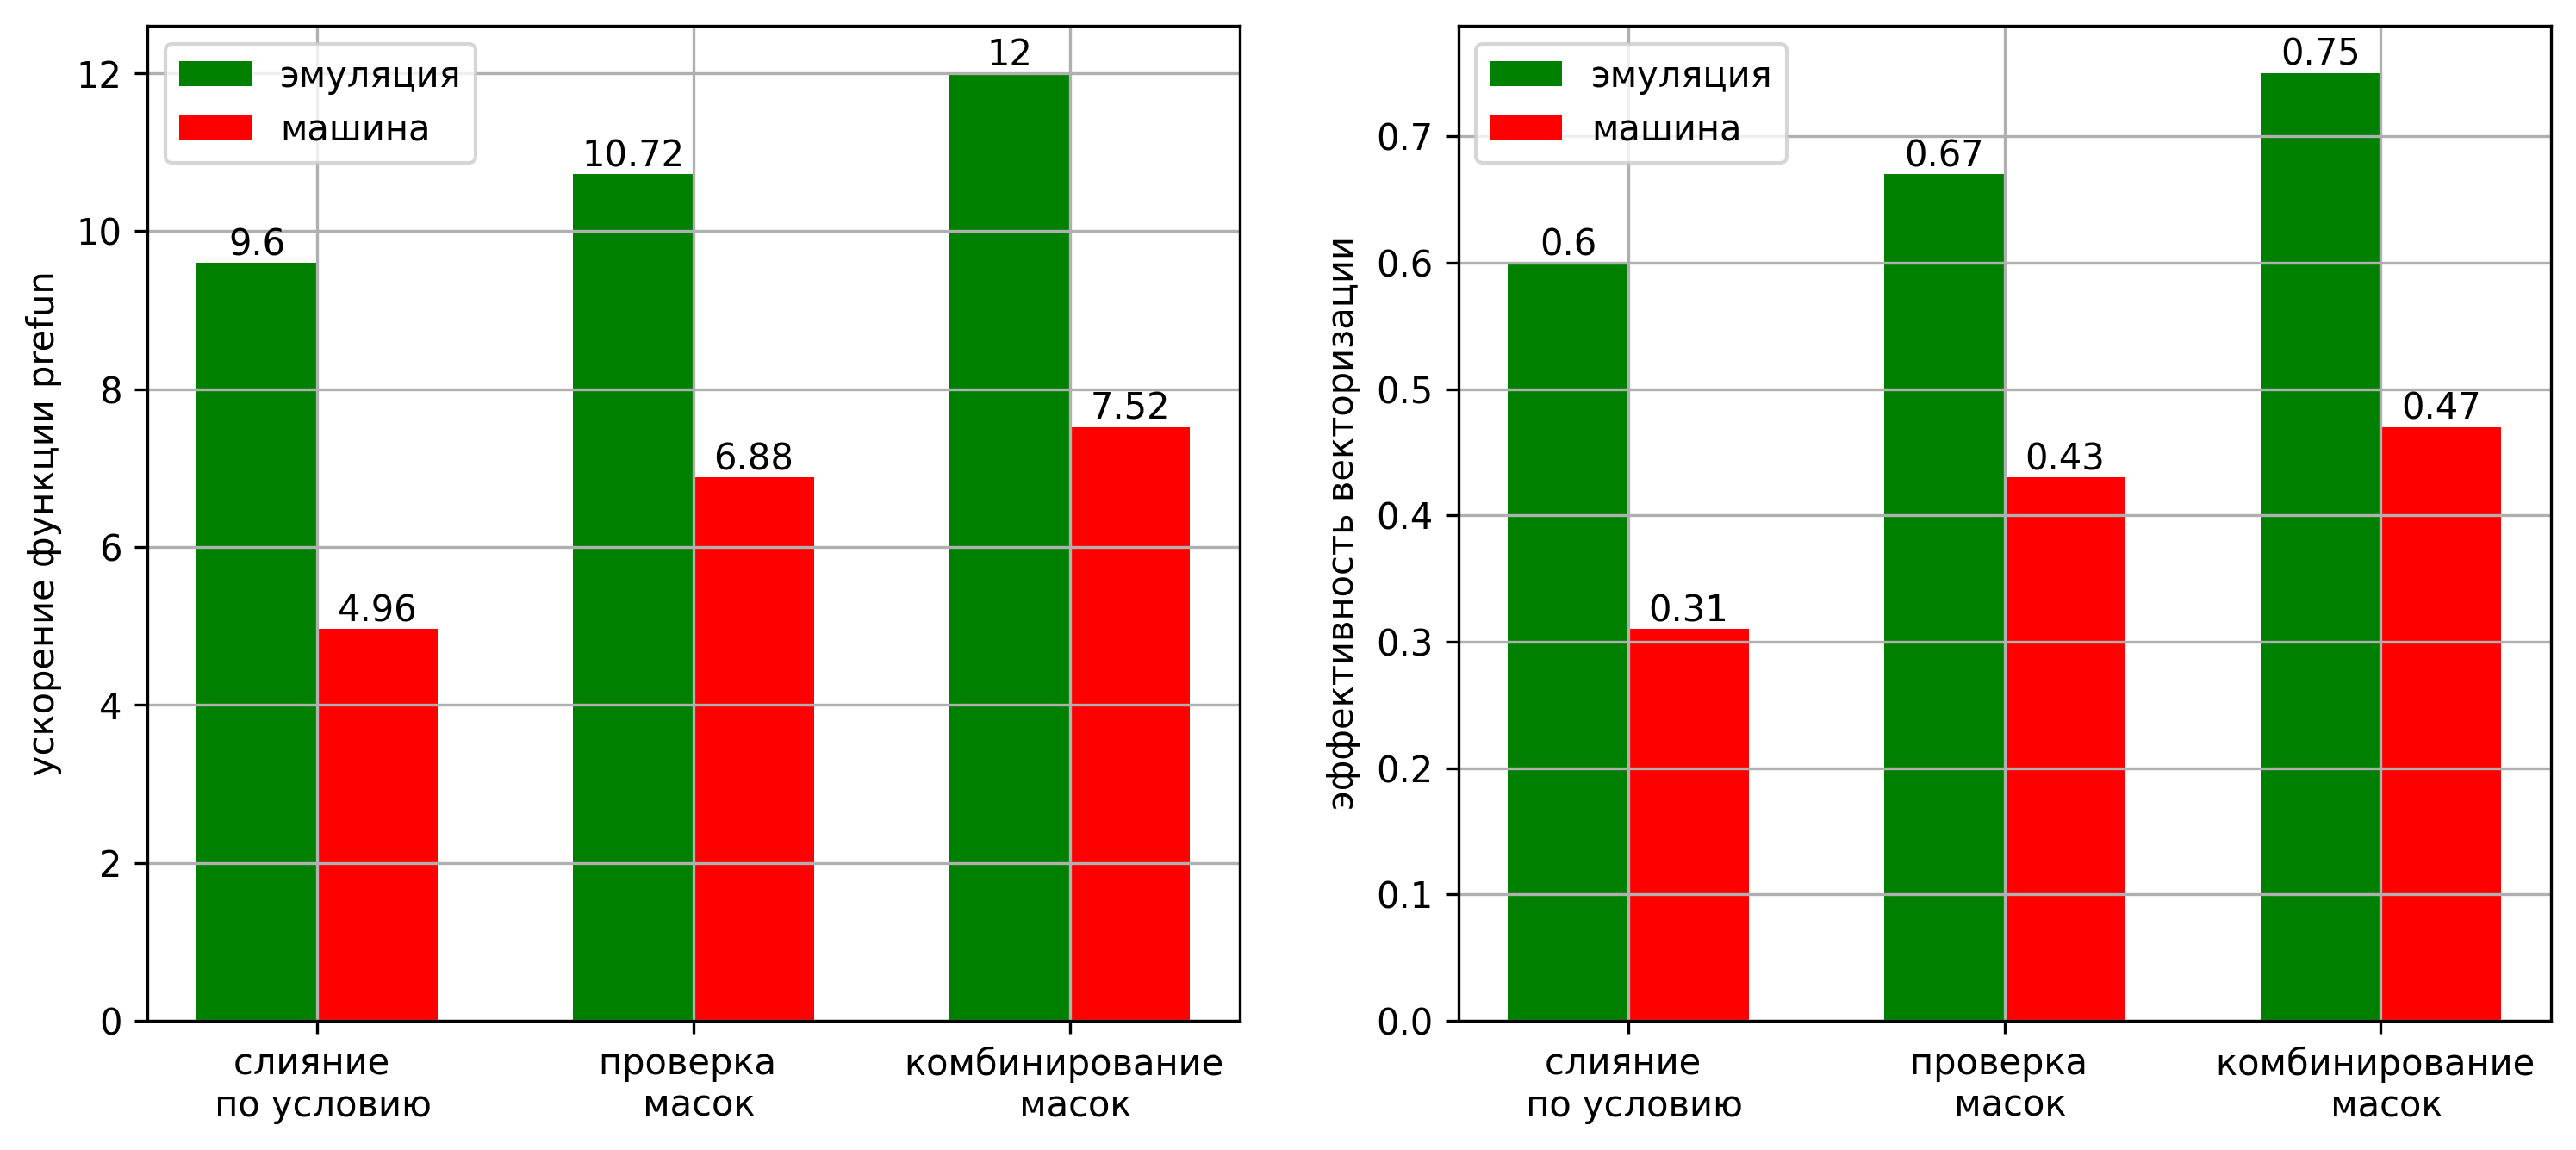
\includegraphics[width=1.0\textwidth]{./pics/text_4_vec_comb_mask/res.png}
\singlespacing
\captionstyle{center}\caption{Результаты сравнения эффективности векторизации при простом слиянии, с проверкой масок и с объединением масок в режимах эмуляции и на реальной машине.}
\label{fig:text_4_vec_comb_mask_res}
\end{figure}

%----------------------------------

В пп.~4.10~--~4.13 проводится анализ программного контекста в котором тело плоского цикла само содержит гнезда циклов (рис.~\ref{fig:text_4_vec_flat_loop_vec}).
В этих пунктах отдельно рассматриваются различные виды вложенных циклов, и анализируется влияние этих видов на эффективность векторизации.

\begin{figure}[!ht]
\centering
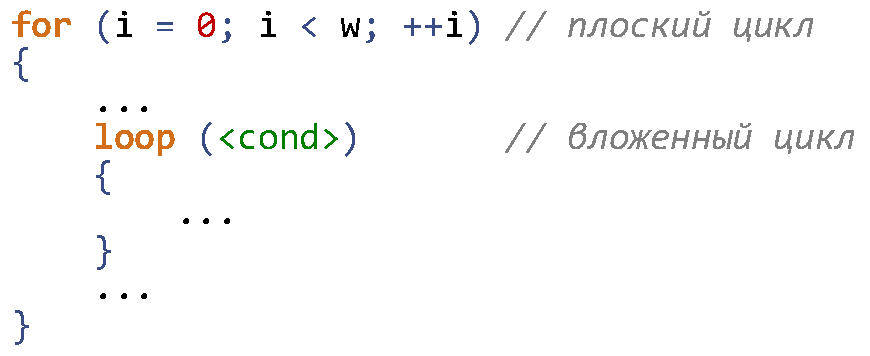
\includegraphics[width=0.6\textwidth]{./pics/text_4_vec_riemann/flat_loop_nest.pdf}
\singlespacing
\captionstyle{center}\caption{Плоский цикл и вложенный в него цикл с произвольным условием выхода.}
\label{fig:text_4_vec_flat_loop_vec}
\end{figure}

В п.~4.10 рассматриваются вложенные \textit{циклы с фиксированным количеством итераций}, то есть условие выхода из которого является константным для векторизуемого плоского цикла.
При векторизации такого программного контекста условие выхода из вложенного цикла переносится в векторизованный код в неизменном виде.

\begin{figure}[ht]
\centering
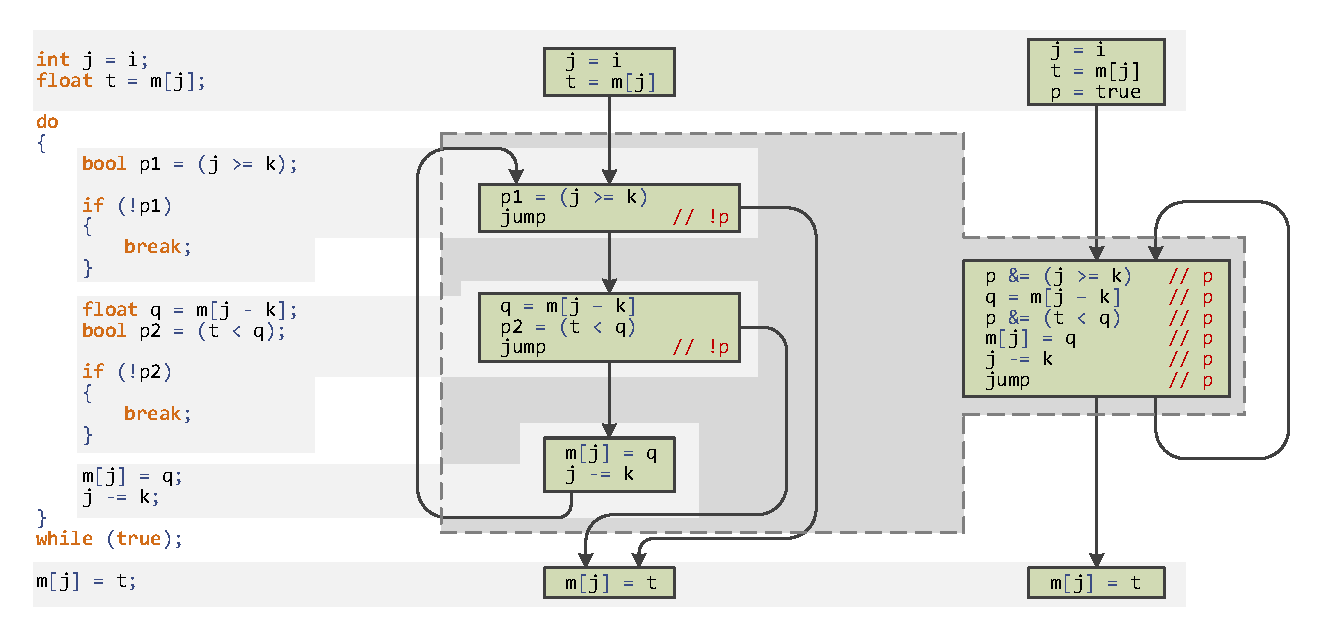
\includegraphics[width=1.0\textwidth]{./pics/text_4_vec_irreg/shell_cfg.pdf}
\singlespacing
\captionstyle{center}\caption{Схема перевода тела вложенного цикла в предикатную форму для последующей векторизации.}
\label{fig:text_4_vec_irreg_shell_cfg}
\end{figure}

В п.~4.11 рассматривается вложенный \textit{цикл с непостоянным количеством итераций}, то есть в котором условие выхода из цикла зависит от номера итерации векторизуемого плоского цикла, но изменяется медленно в зависимости от этого номера.
При векторизации такого программного контекста условие выхода из вложенного цикла трансформируется в векторную маску выполнения тела вложенного цикла, и вложенный цикл продолжает исполняться до тех пор, пока эта векторная маска не истощится.
Основной причиной потери производительности при векторизации такого программного контекста является выполнение итераций вложенного цикла под маской низкой плотности.

\begin{figure}[!ht]
\centering
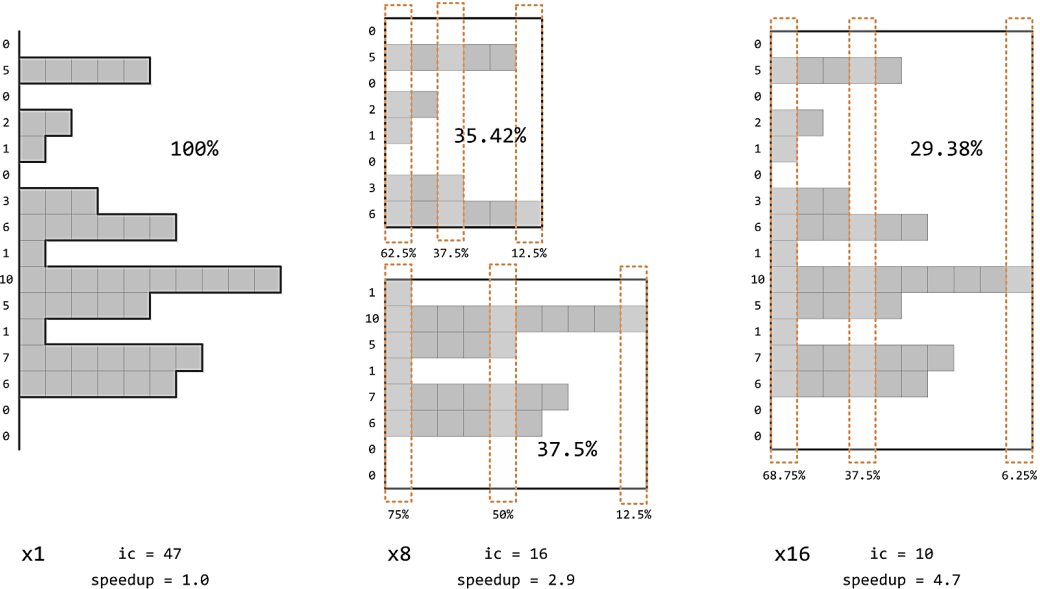
\includegraphics[width=0.8\textwidth]{./pics/text_4_vec_irreg/pack.png}
\singlespacing
\captionstyle{center}\caption{Иллюстрация потери производительности для вложенного цикла с нерегуярным количеством итераций.}
\label{fig:text_4_vec_irreg_pack}
\end{figure}

\begin{figure}[!ht]
\centering
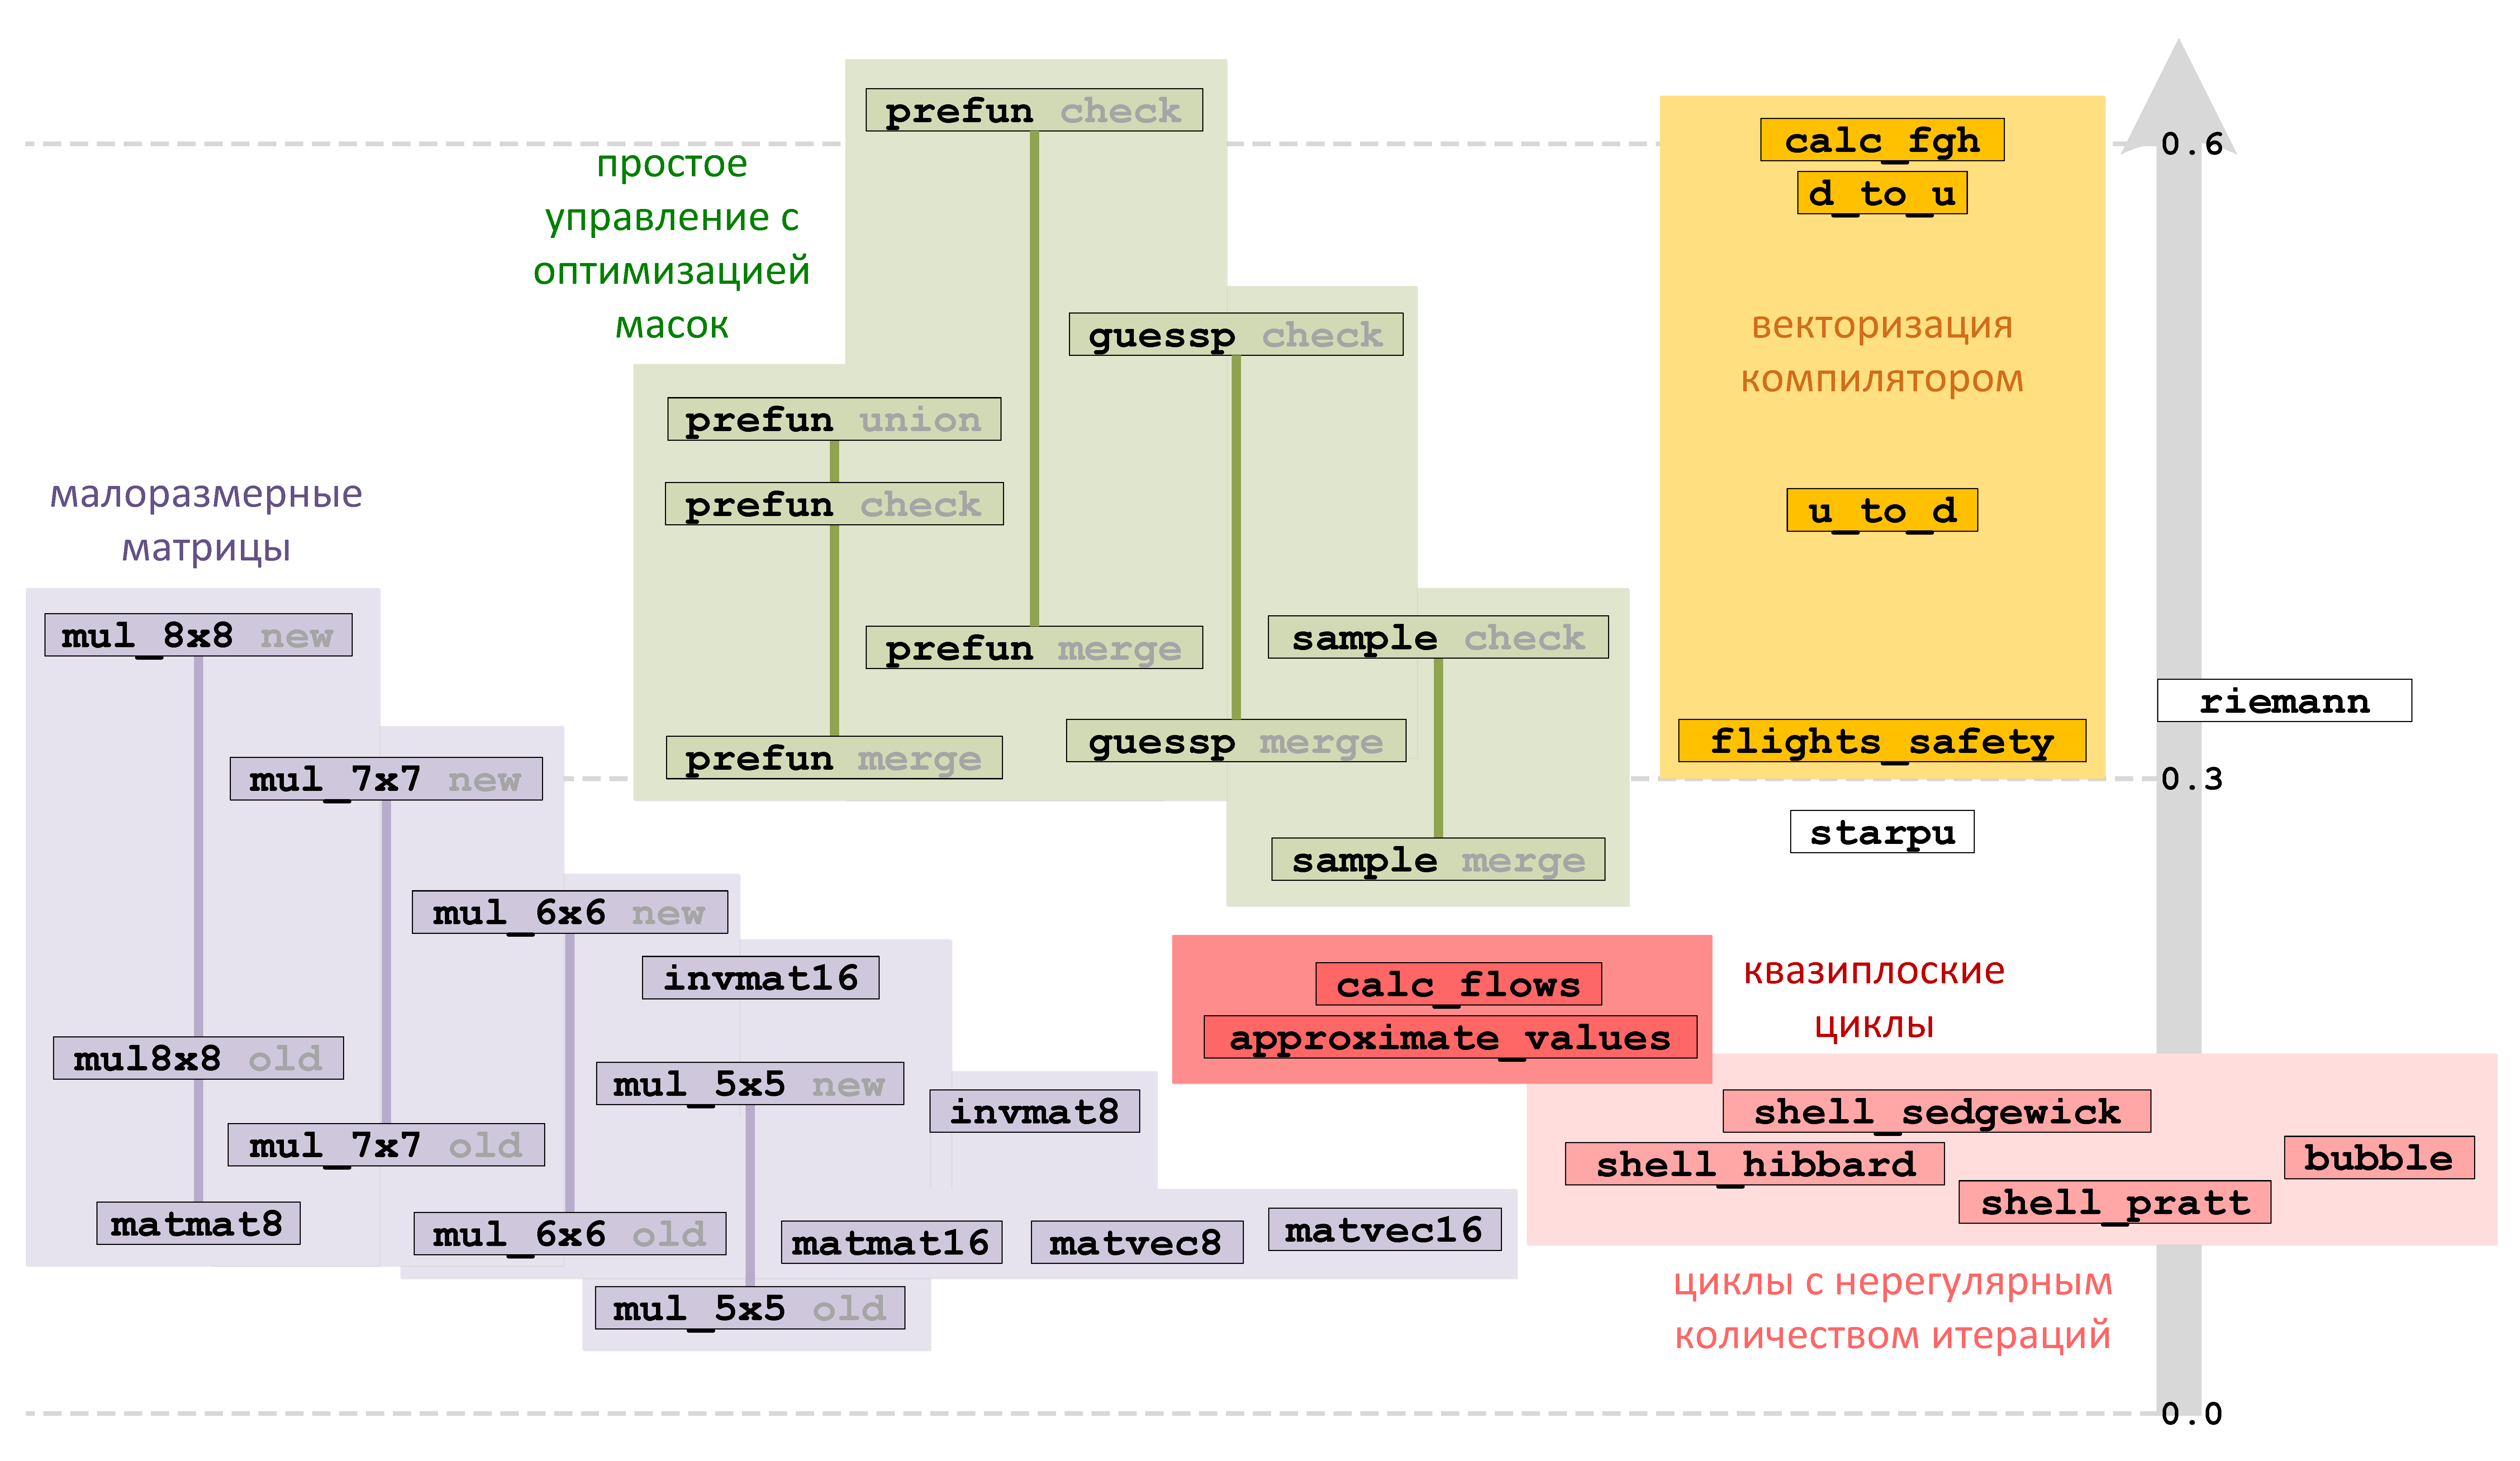
\includegraphics[width=1.0\textwidth]{./pics/text_4_fin/map_cut.pdf}
\singlespacing
\captionstyle{center}\caption{Карта эффективности векторизации.}
\label{fig:text_4_fin_map}
\end{figure}

В п.~4.12 и п.~4.13 рассматривается вещественный и целочисленный программный контекст в котором вложенный цикл характеризуется как \textit{цикл с нерегулярным количеством итераций}, то есть условие выхода из вложенного цикла не только не зависит от номера итерации плоского цикла, но эта зависимость носит стохастический характер.
При векторизации такого программного контекста плотность маски выполнения вложенного цикла является крайне низкой, что приводит к наиболее серьезной потери производительности (рис.~\ref{fig:text_4_vec_irreg_pack}). 

%----------------------------------

В выводах из главы приводится общая карта рассмотренного в главе векторизованного программного контекста, представленная на рис.~\ref{fig:text_4_fin_map}.

Из карты делается вывод, что наиболее неудобным программным контекстом для векторизации являются гнезда циклов с нерегулярным количеством итераций, а также \textit{квазиплоские циклы}, то есть циклы, нарушающие некоторые требования, предъявляеимые к плоским циклам (дополнительная косвенность при обращении в память, невыровненность данных и другие).
Наиболее удобным контекстом для векторизации являются плоские циклы с простым управлением и применением проверок и объединения масок.

%---------------------------------------------------------------------------------------------------

\end{document}
